
\chapter{超弹道光范围光学成像方法}
生活中,我们观察物体、辨别物体总是遵循“光沿直线传播”、“所见即所得”的传统光学成像规律,常见的视觉成像系统像人眼、照相机以及光学成像工具如放大镜、显微镜和望远镜等都以此为物理基础。传统光学成像主要通过提取弹道光(或抑制散射光)的方式解决透过无散射(或者弱散射)介质的成像问题。当光透过生物组织、烟尘和云雾等强散射介质时,传统光学成像规律失效。其主要原因是光在强散射介质中传播时,介质中大小为波长量级的粒子对入射光波产生的散射作用使原本有序的波前相位产生严重畸变,出射光场变得随机且紊乱,最终在观测面上只能接收到散斑图案,难以实现对目标的观测或成像。因此,散射效应成为制约透过散射介质成像技术发展的瓶颈和关键问题。

近年来,随着计算机技术飞速发展、介观物理研究的深入、计算成像思想的完善和图像处理技术的发展,形成以物理机制为基础的计算光学成像技术。计算光学成像技术作为新型成像手段,不仅推动了传统成像的发展,而且在解决散射成像方面表现出了得天独厚的优势。经过各国科学家们的不懈努力,计算成像理论以及相关实验技术迅速发展,取得了许多突破性研究成果。在弹道光提取方面,如:自适应光学成像技术 (Adaptive optics technique)、门选通技术、光学相干层析(Optical coherence tomography)\cite{huang_optical_1991}、共聚焦显微 (Confocal microscopy)\cite{webb_confocal_1996}、多光子显微 (Multiphoton microscopy)\cite{denk_two_photon_1990,helmchen_deep_2005}、光声显微 (Optoacoustic microscopy)\cite{zhang_functional_2006,wang_multiscale_2009}、复合荧光分子层析 (Hybrid fluorescence molecular tomography)\cite{ale_fmt_xct_2012}、多光谱光声层析 (Multispectral optoacoustic tomography)\cite{razansky_volumetric_2011,ntziachristos_going_2010} 等光学成像技术的发展及应用,解决了天文成像、水下探测和生物成像等领域的关键问题。在散射光利用方面:随着空间光调制器 (Spatial light modulator,SLM)、数字微镜器件 (Digital micromirror device,DMD)、微机电系统调制器 (Micro electro mechanical system,MEMS) 等数字波前整形器件的出现,促使了计算成像技术和散射成像技术有机的结合,涌现出了许多新型光学成像技术,如:光学相位共轭 (Optical phase conjugation)、波前反馈调节 (Wavefront shaping technique)、基于光学传输矩阵 (Transmission matrix) 等,极大地促进了散射成像技术在显微成像领域的应用。与此同时,随着对光学记忆效应 (Optical memory effect) 的深入研究,散斑相关成像技术 的提出为透过散射介质成像打开了崭新的局面。随着计算光学成像的进一步发展,基于点扩散函数 (Point Spread Function, PSF) 工程 和深度学习 的方法,也成为了解决透过散射介质成像的重要途径。

纵观散射成像的发展历程,随着对散射机理研究的不断深入,散射成像技术已从早期基础理论研究到实验室下模型验证研究再到透过散射介质成像应用研究。早期的散射成像技术注重于克服散射或抑制散射,通过弹道光与散射光的分离,最终获取有效的目标信息。现阶段的散射成像技术侧重于散射光的利用,充分挖掘散射光的特性,实现从不可探测到可探测质的飞跃。值得注意的是,散射成像技术不仅在显微成像和超分辨成像方面有着广泛的应用,而且也将在全息成像、光纤成像和光通讯等领域扮演着重要的角色。

现有透过散射介质成像方法主要有波前整形和基于光学记忆效应的散射成像技术。波前整形技术,包含光学相位共轭、基于反馈优化的波前整形和光学传输矩阵技术三部分,该技术主要研究光波在介质中的传播规律以及特性,为散射效应的利用奠定基础。基于光学记忆效应的散射成像技术,包含散斑相关成像技术和点扩散函数工程成像技术两部分,该技术核心在于对于散斑能量的利用,利用的散斑分布特点实现透过散射介质成像及相关工作。本文分别对以上方法在散射成像相关成果以及进展进行归纳和总结,并对未来的发展趋势进行了分析与展望。

\section{基于波前整形的散射成像技术}

在散射介质中传播受到散射效应的影响,在像面形成系列散斑。如何定量或定性描述散射介质在光传播过程中的影响成为利用光散射效应的关键问题。虽然光在多重散射介质中传播具有很高的随机性,但当散射介质处稳定于状态时,光在散射介质中的传播具有确定性。散射介质的特性可以与多模光纤进行类比,其输出光场可看作多种模式之间的耦合与叠加。为了精确地描述散射介质在光传播过程的作用,光学传输矩阵思想被提出,有效地将入射光场和出射光场联系起来。近年来,随着光散射理论和实验技术的飞速发展,研究人员基于光学相位共轭、反馈优化的波前整形和光学传输矩阵等技术,实现了透过散射介质的聚焦或者成像。在未获得完善的光学传输矩阵的前提下,为实现透过散射介质聚焦或成像,通常采用光学相位共轭技术或者基于反馈优化的波前整形技术;在测得完备的光学矩阵之后,往往利用光学传输矩阵技术能够有效地实现对出射光场的控制。研究结果表明,波前整形技术在生物医学成像、超分辨成像和光通信等方面有着巨大的应用前景。

\subsection{光学相位共轭}

光学相位共轭技术是时间反演技术在光学领域的应用,最早的光学相位共轭技术通过在照相板上记录全息图来实现。本质上,光学相位共轭技术利用光传播的可逆性,通过获得透过介质后的光场分布,反向输入透射光场的相位共轭波形,重建原始的入射光场。光学相位共轭实现可以分为两步:第一步,光场信息的记录;第二步,相位共轭光的生成。按照相位共轭光产生方式的不同,光学相位共轭技术可以分为非线性光学相位共轭技术和数字光学相位共轭技术两类。前者可以使用数字全息或定量相位成像技术来实现,后者是空间光调制器实现。在实验中,我们通常只能获取介质一面光场信息(或者获取部分入射光和部分散射光),在多重散射材料的情况下(也在混沌腔的情况)甚至有限的相位共轭也可以地重建部分的入射光场信息。
依据非线性过程的差异,非线性光学相位共轭技术可以分为:三波混频相位共轭技术、四波混频相位共轭技术、受激布里渊散射相位共轭技术和光折变晶体相位共轭技术。总体而言,非线光学相位共轭技术实施起来比较复杂,通常需要非线性晶体、特定波长和强激光光源。虽然实施起来比较复杂,但是非线性相位共轭技术自早期以来多用于透过复杂介质聚焦。光折变晶体作为光学相位共轭技术的一种常用手段,虽然其调节速度较慢,但可实现透过厚生物组织的聚焦成像。随着材料技术的飞速发展,许多新型光学共轭材料被研发出来,其调节速度可与SLM相媲美。许多增益介质能够提供快速的光学共轭调节,但受到其物理效应的限制,仅适用于窄谱光源。三波混频相位共轭技术具有速度快频带宽的特点,但其有效角度较小。与数字光学相位共轭技术相比,非线性光学相位共轭技术在模式耦合效率方面具有较大优势,往往高出$1 \sim 2$数量级。因此非线性光学相位共轭技术在生物医学方面仍然具有很大的潜力。

\begin{figure}[htp]
	\centering
	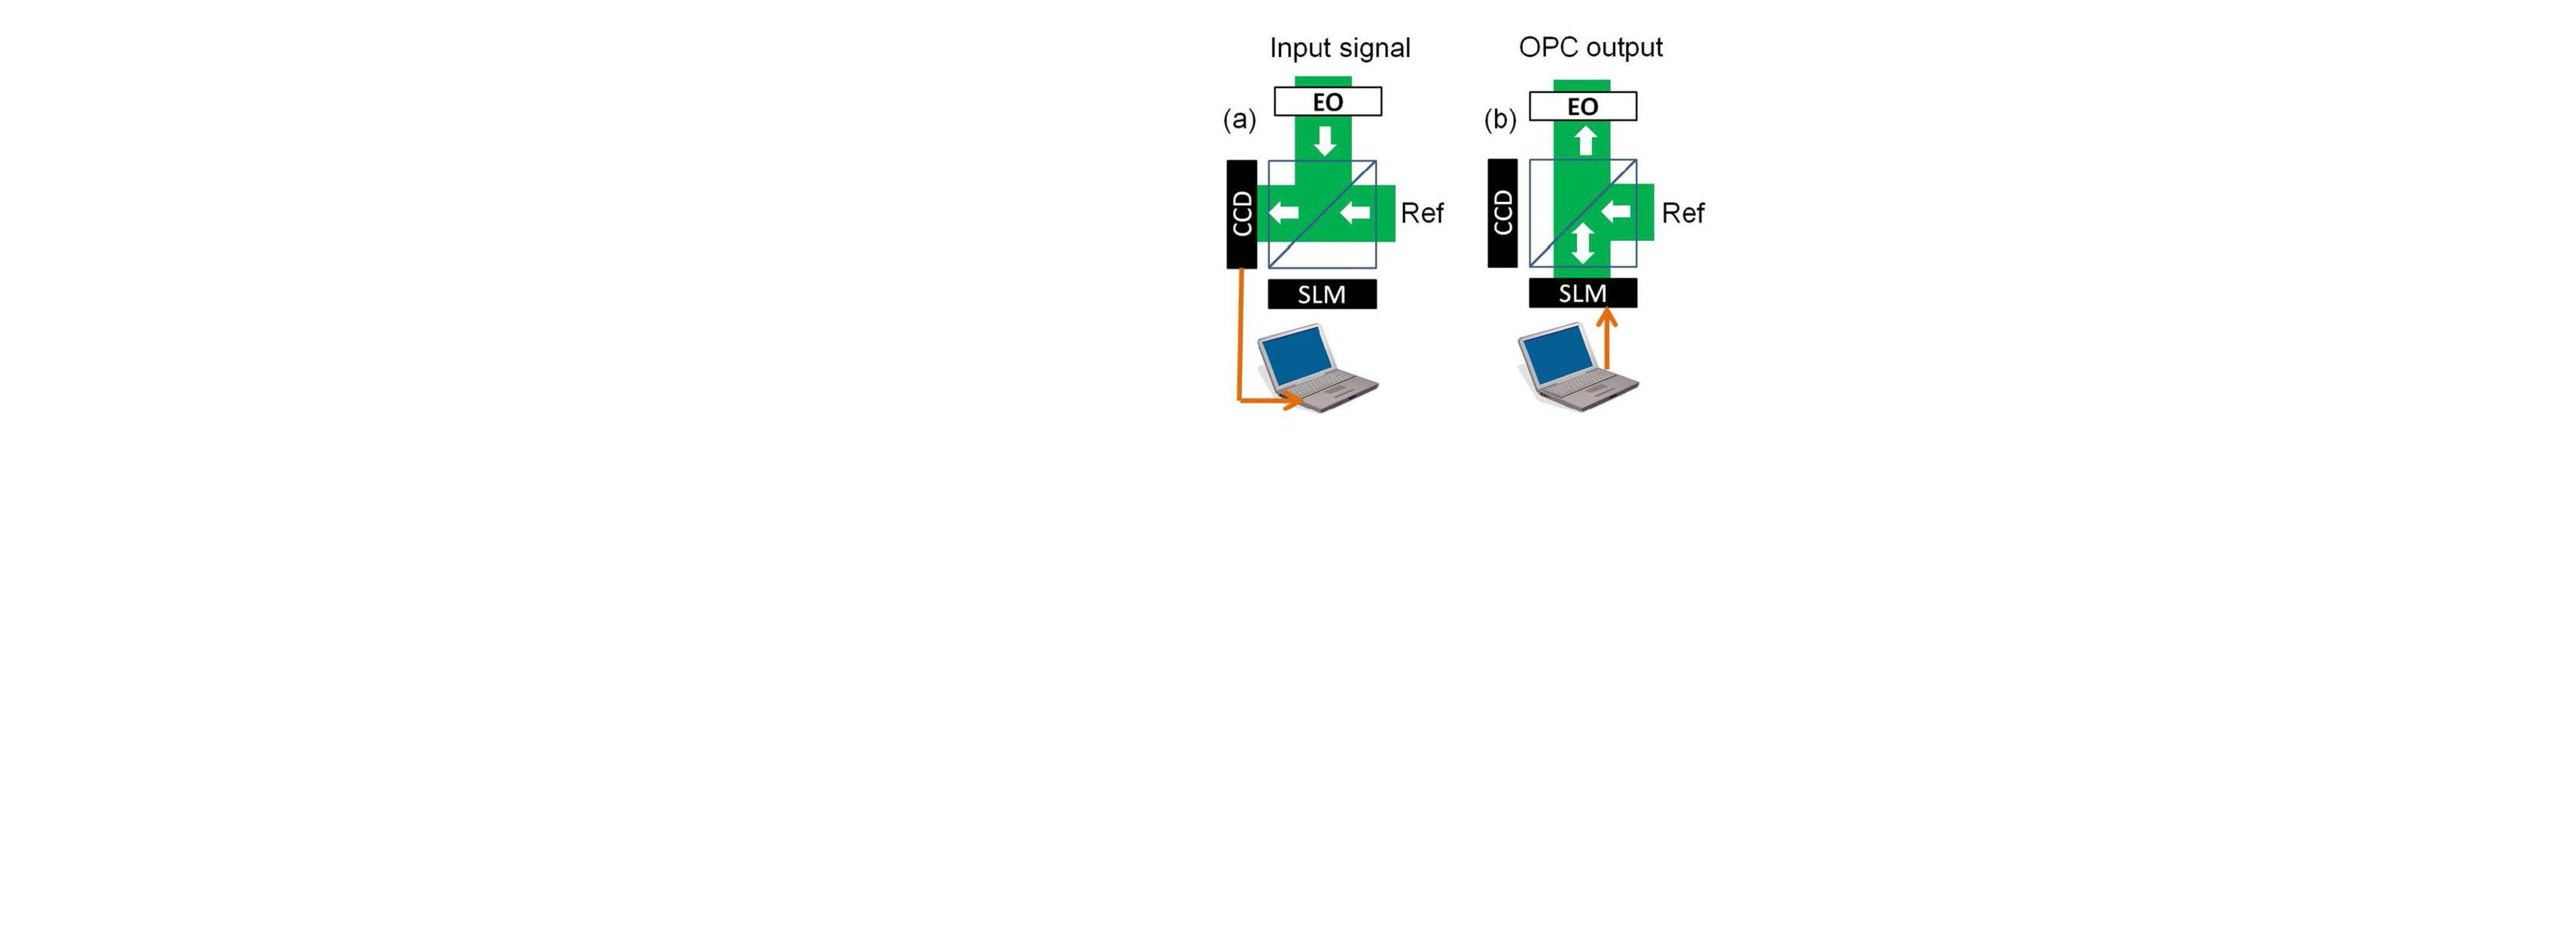
\includegraphics[scale=0.7]{C2.fig1}
	\caption{数字光学相位共轭示意图}
	\label{fig2:1}
\end{figure}

由于SLM和DMD等元件的出现,使数字光学相位共轭调制变成可能,数字光学相位共轭技术的工作原理如图\ref{fig2:1}所示。在获得输出场的光场信息后,利用数字元器件产生相位共轭光,进而实现透过散射介质的聚焦和成像。2008年,Z. Yaqoob等人首次提出了一种基于光学相位共轭的散射成像模型,通过单次记录光场信息克服介质的散射实现成像。2009年,Pauriss等人利用了数字光学相位共轭技术实现了对光纤输出光场的控制和补偿。随后,数字光学相位共轭技术被应用于透过散射介质和多模光纤聚焦。

数字光学相位共轭技术虽然在调制效率方面具有劣势,但是对于透过复杂介质成像方面的应用有着得天独厚的优势。数字光学相位共轭技术利用计算机记录其输出光场分布,利用调制器生成共轭光,可以对无数个输入光场进行重构,相较而言,非线性光学相位共轭技术不具备此特点。在未来发展中,如何提高数字光学相位共轭技术的效率问题,将决定数字光学相位共轭技术在未来应用中的地位。

\subsection{基于反馈优化波前整形的散射介质成像技术}

基于反馈优化的波前整形技术利用优化算法(非线性或线性),通过迭代获取到目标光场所对应的最优波前,从而实现透过散射介质聚焦或成像。本质上,基于反馈优化的波前整形技术将散射介质对于光场的调制过程看作“黑箱”处理,通过迭代算法获取相应的波前,进而实现了对于输出光场的模式以及不同模式之间耦合的控制。

2007年,A. P. Mosk课题组利用SLM对入射到随机散射介质中的光波进行波前相位调制,采用反馈控制算法对空间光调制器的SLM像素进行逐个优化,通过不断迭代的方式获取最优波前,所得的最优波前幅值或相位可以适当补偿由介质散射引起的波前畸变,最终得到了亮度高于调制前散斑1000倍的聚焦光斑,远远优于光学透镜的聚焦效果,实验装置和实验结果分别如图\ref{fig2:2}和图\ref{fig2:3}所示。图\ref{fig2:2}中,图\ref{fig2:2}(a)为未波前整形前示意图;图\ref{fig2:2}(b)为波前整形后示意图。图\ref{fig2:3}中,图\ref{fig2:3}(a)为聚焦前散斑;图\ref{fig2:3}(b)为单点聚焦结果;图\ref{fig2:3}(c)为多点聚焦结果;图\ref{fig2:3}(d)为优化后的波前相位图。

\begin{figure}[htp]
	\centering
	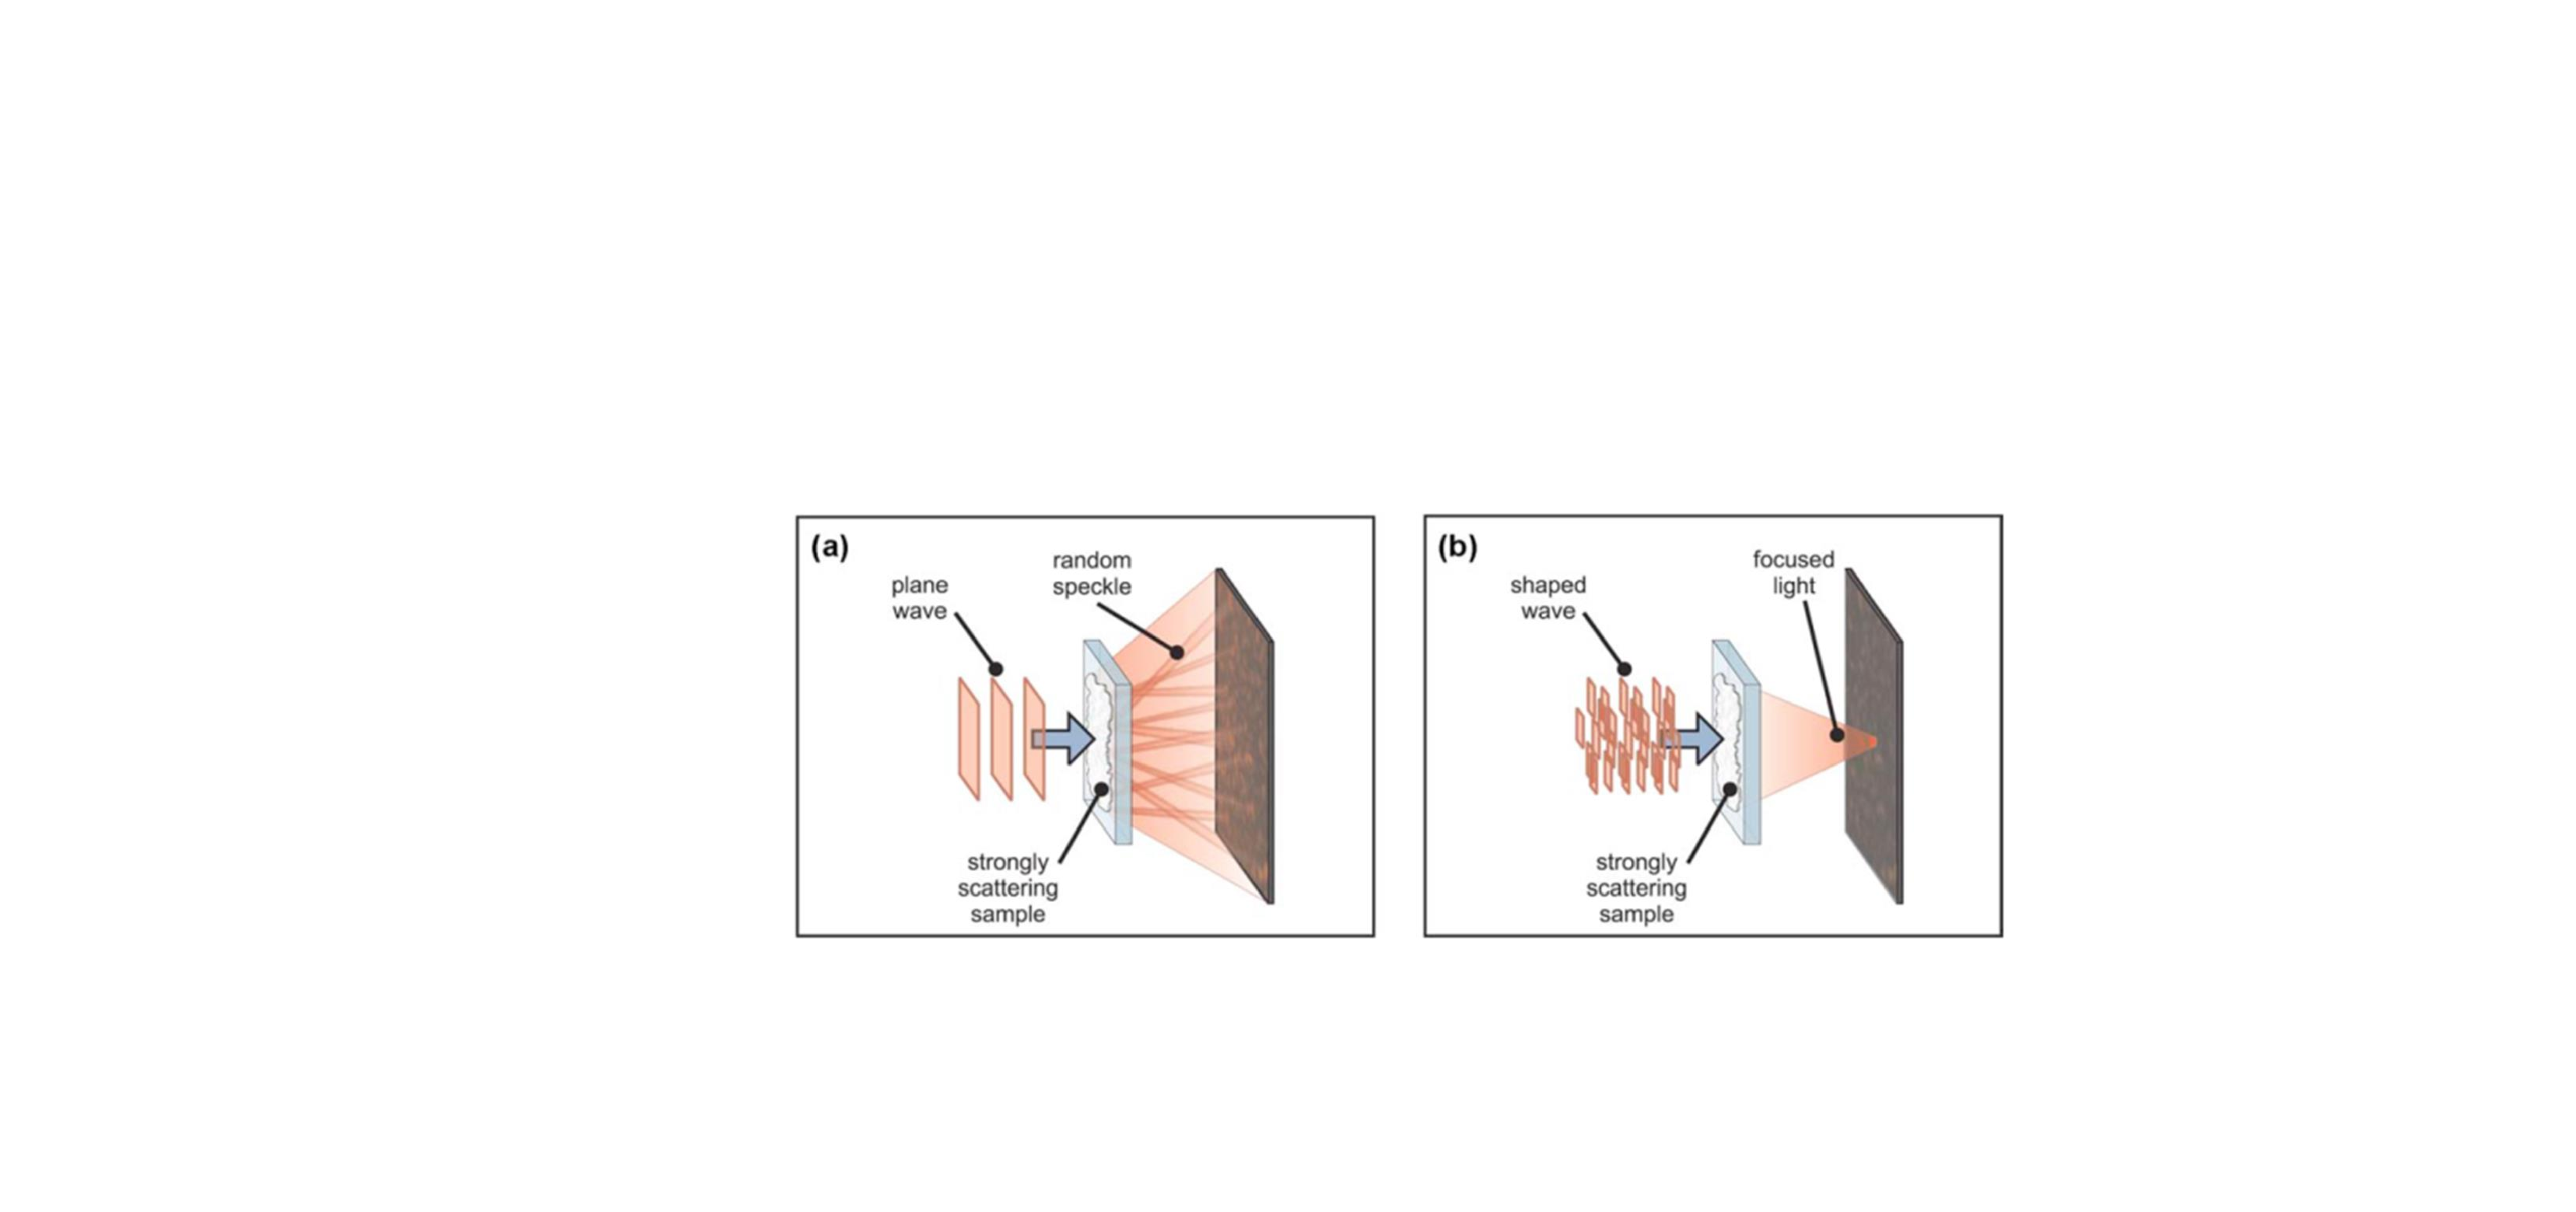
\includegraphics[scale=0.35]{C2.fig2}
	\caption{波前整形示意图}
	\label{fig2:2}
\end{figure}

\begin{figure}[htp]
	\centering
	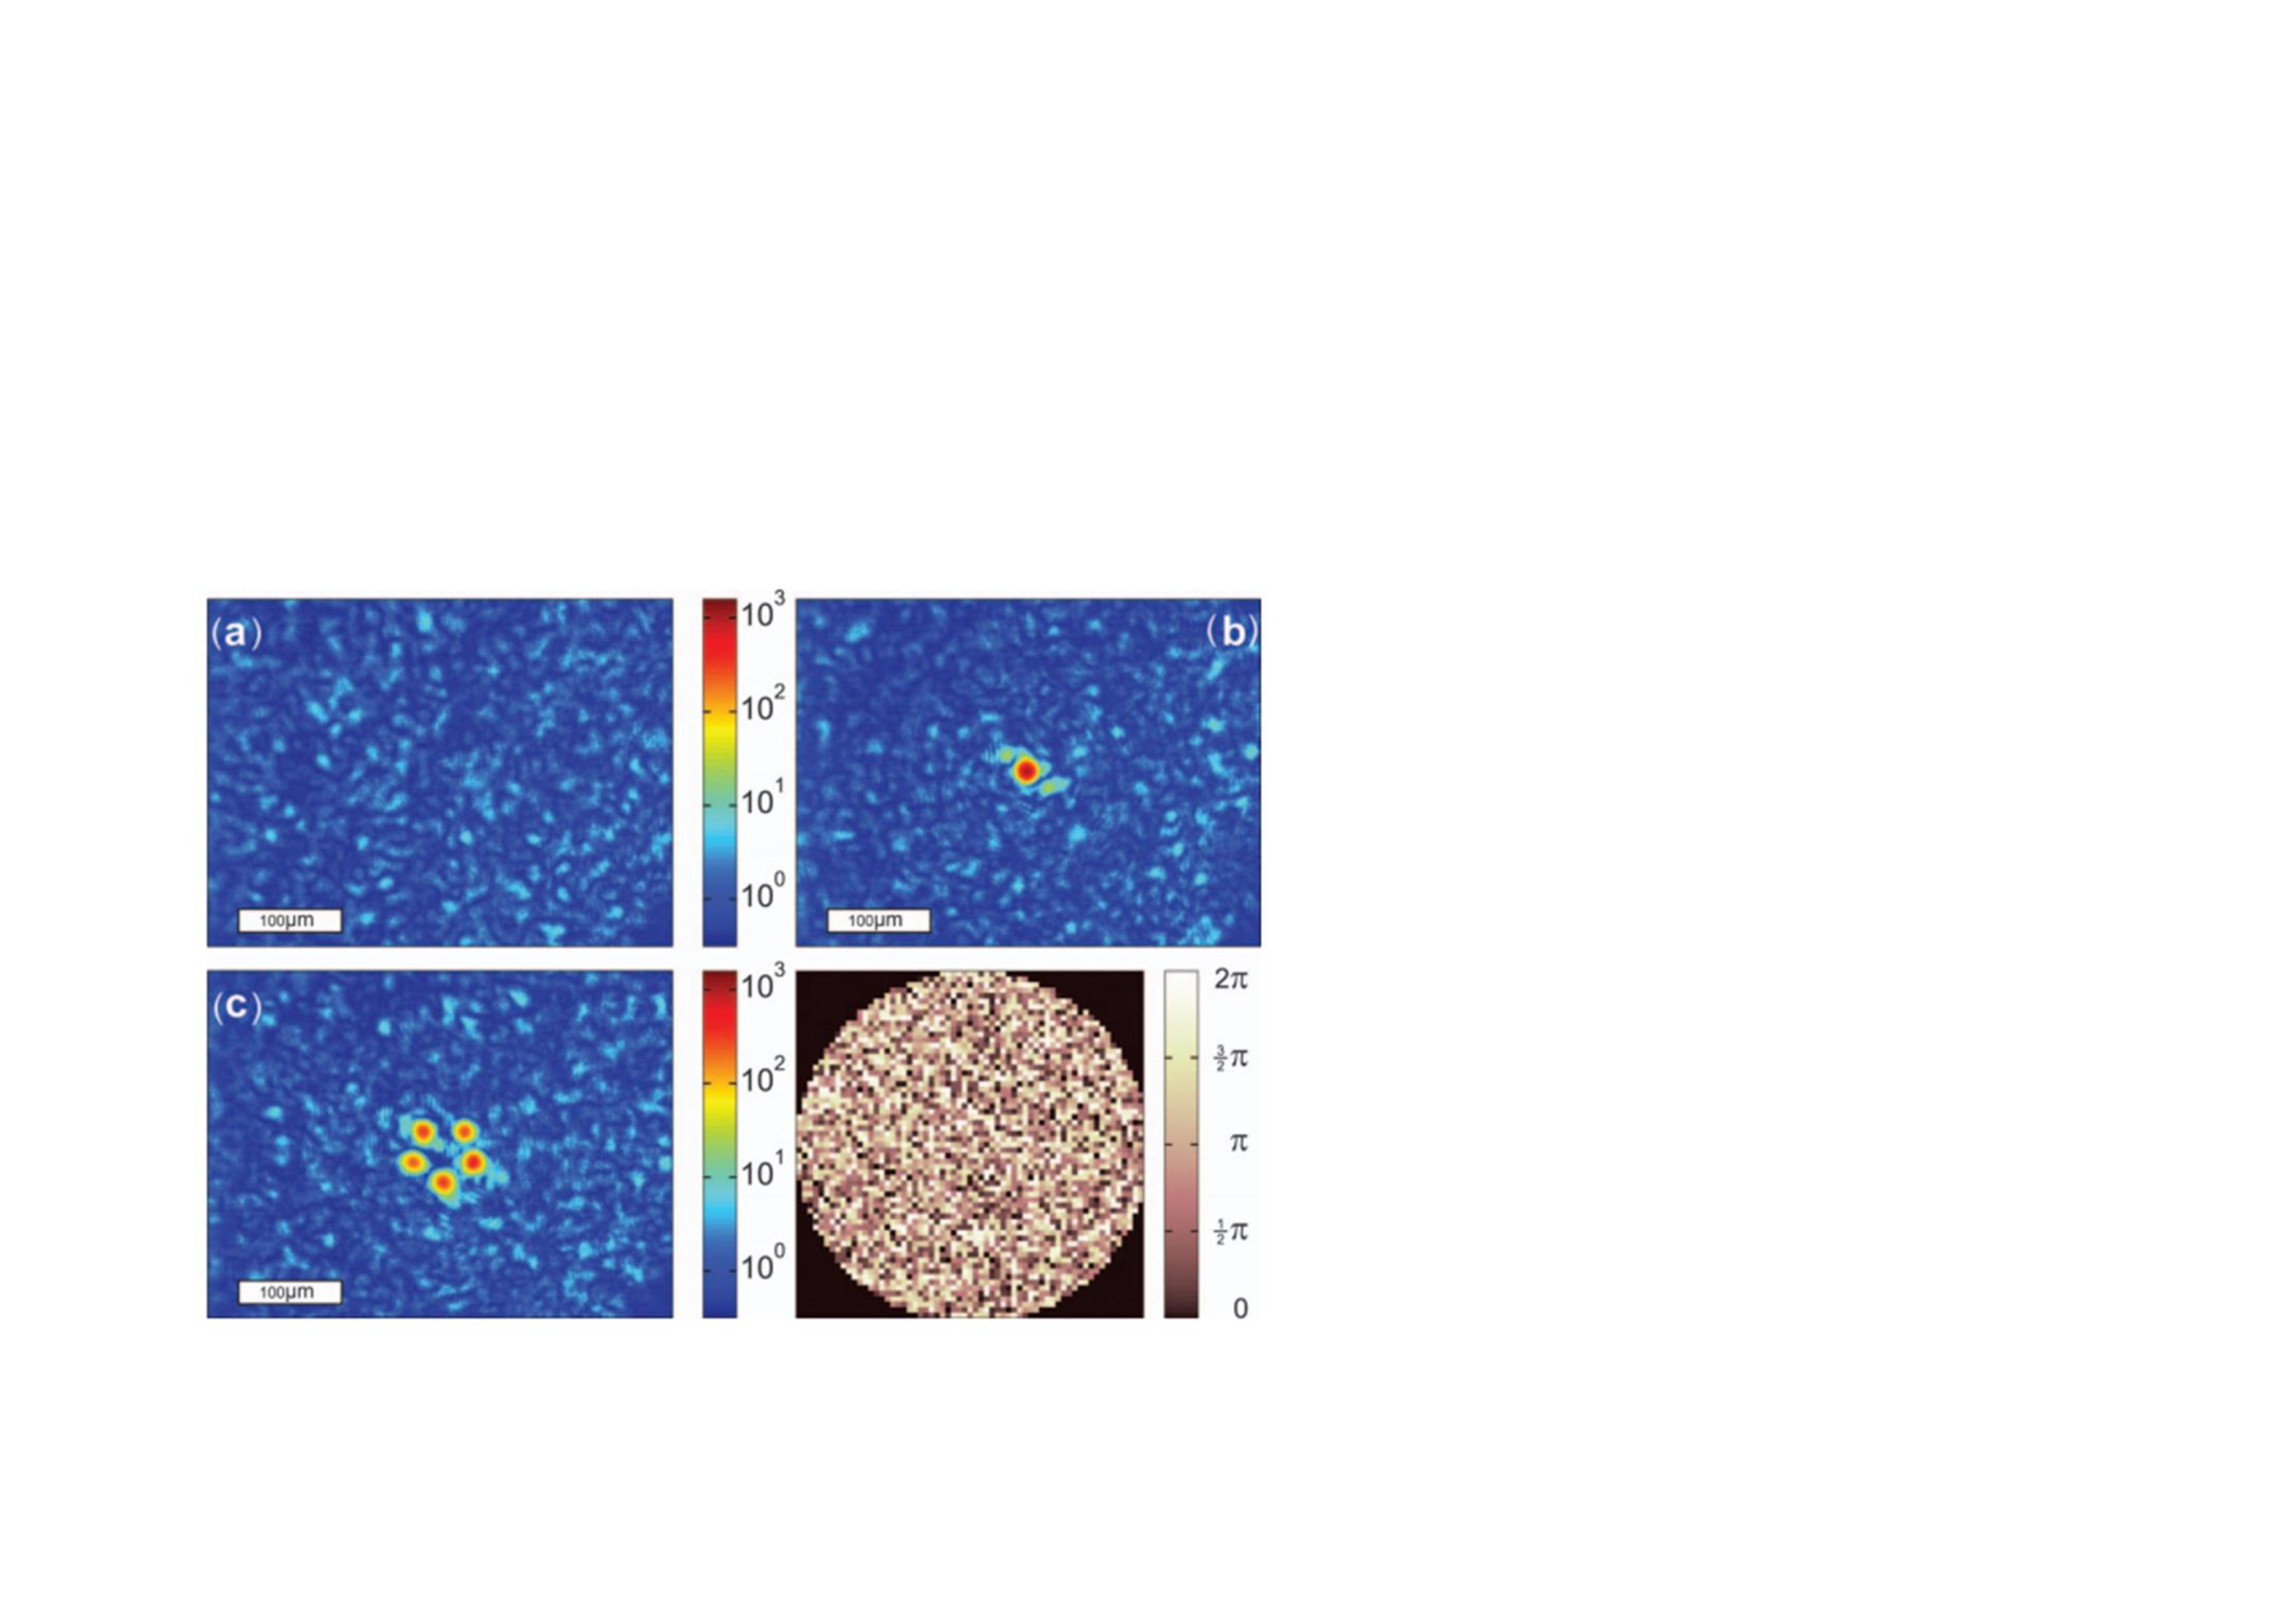
\includegraphics[scale=0.40]{C2.fig3}
	\caption{波前整形聚焦结果}
	\label{fig2:3}
\end{figure}

2010年,Mosk课题组通过在传统透镜光学系统后面放置一块厚度为6 μm的散射介质(如图\ref{fig2:4}所示,图\ref{fig2:4}(a)为传统透镜聚焦光学系统;图\ref{fig2:4}(b)为随机散射介质聚焦光学系统),利用反馈优化的波前整形方法获得了直径仅为传统光学系统1/10的聚焦光斑,极大地提升了光学系统的分辨率,实现了超衍射极限聚焦,如图\ref{fig2:5}所示,图\ref{fig2:5}(a)为传统透镜光学系统聚焦光斑;图\ref{fig2:5}(b)为随机散射介质光学系统调制的前散斑;图\ref{fig2:5}(c)为超衍射极限聚焦光斑;图\ref{fig2:5}(d)为优化的波前相位。该项工作充分利用了随机散射介质的随机散射特性,随机散射介质可以增大原有光学系统的数值孔径,从而使所获得的焦斑尺寸能超越传统透镜的光学衍射极限,具有划时代的意义。

\begin{figure}[htp]
	\centering
	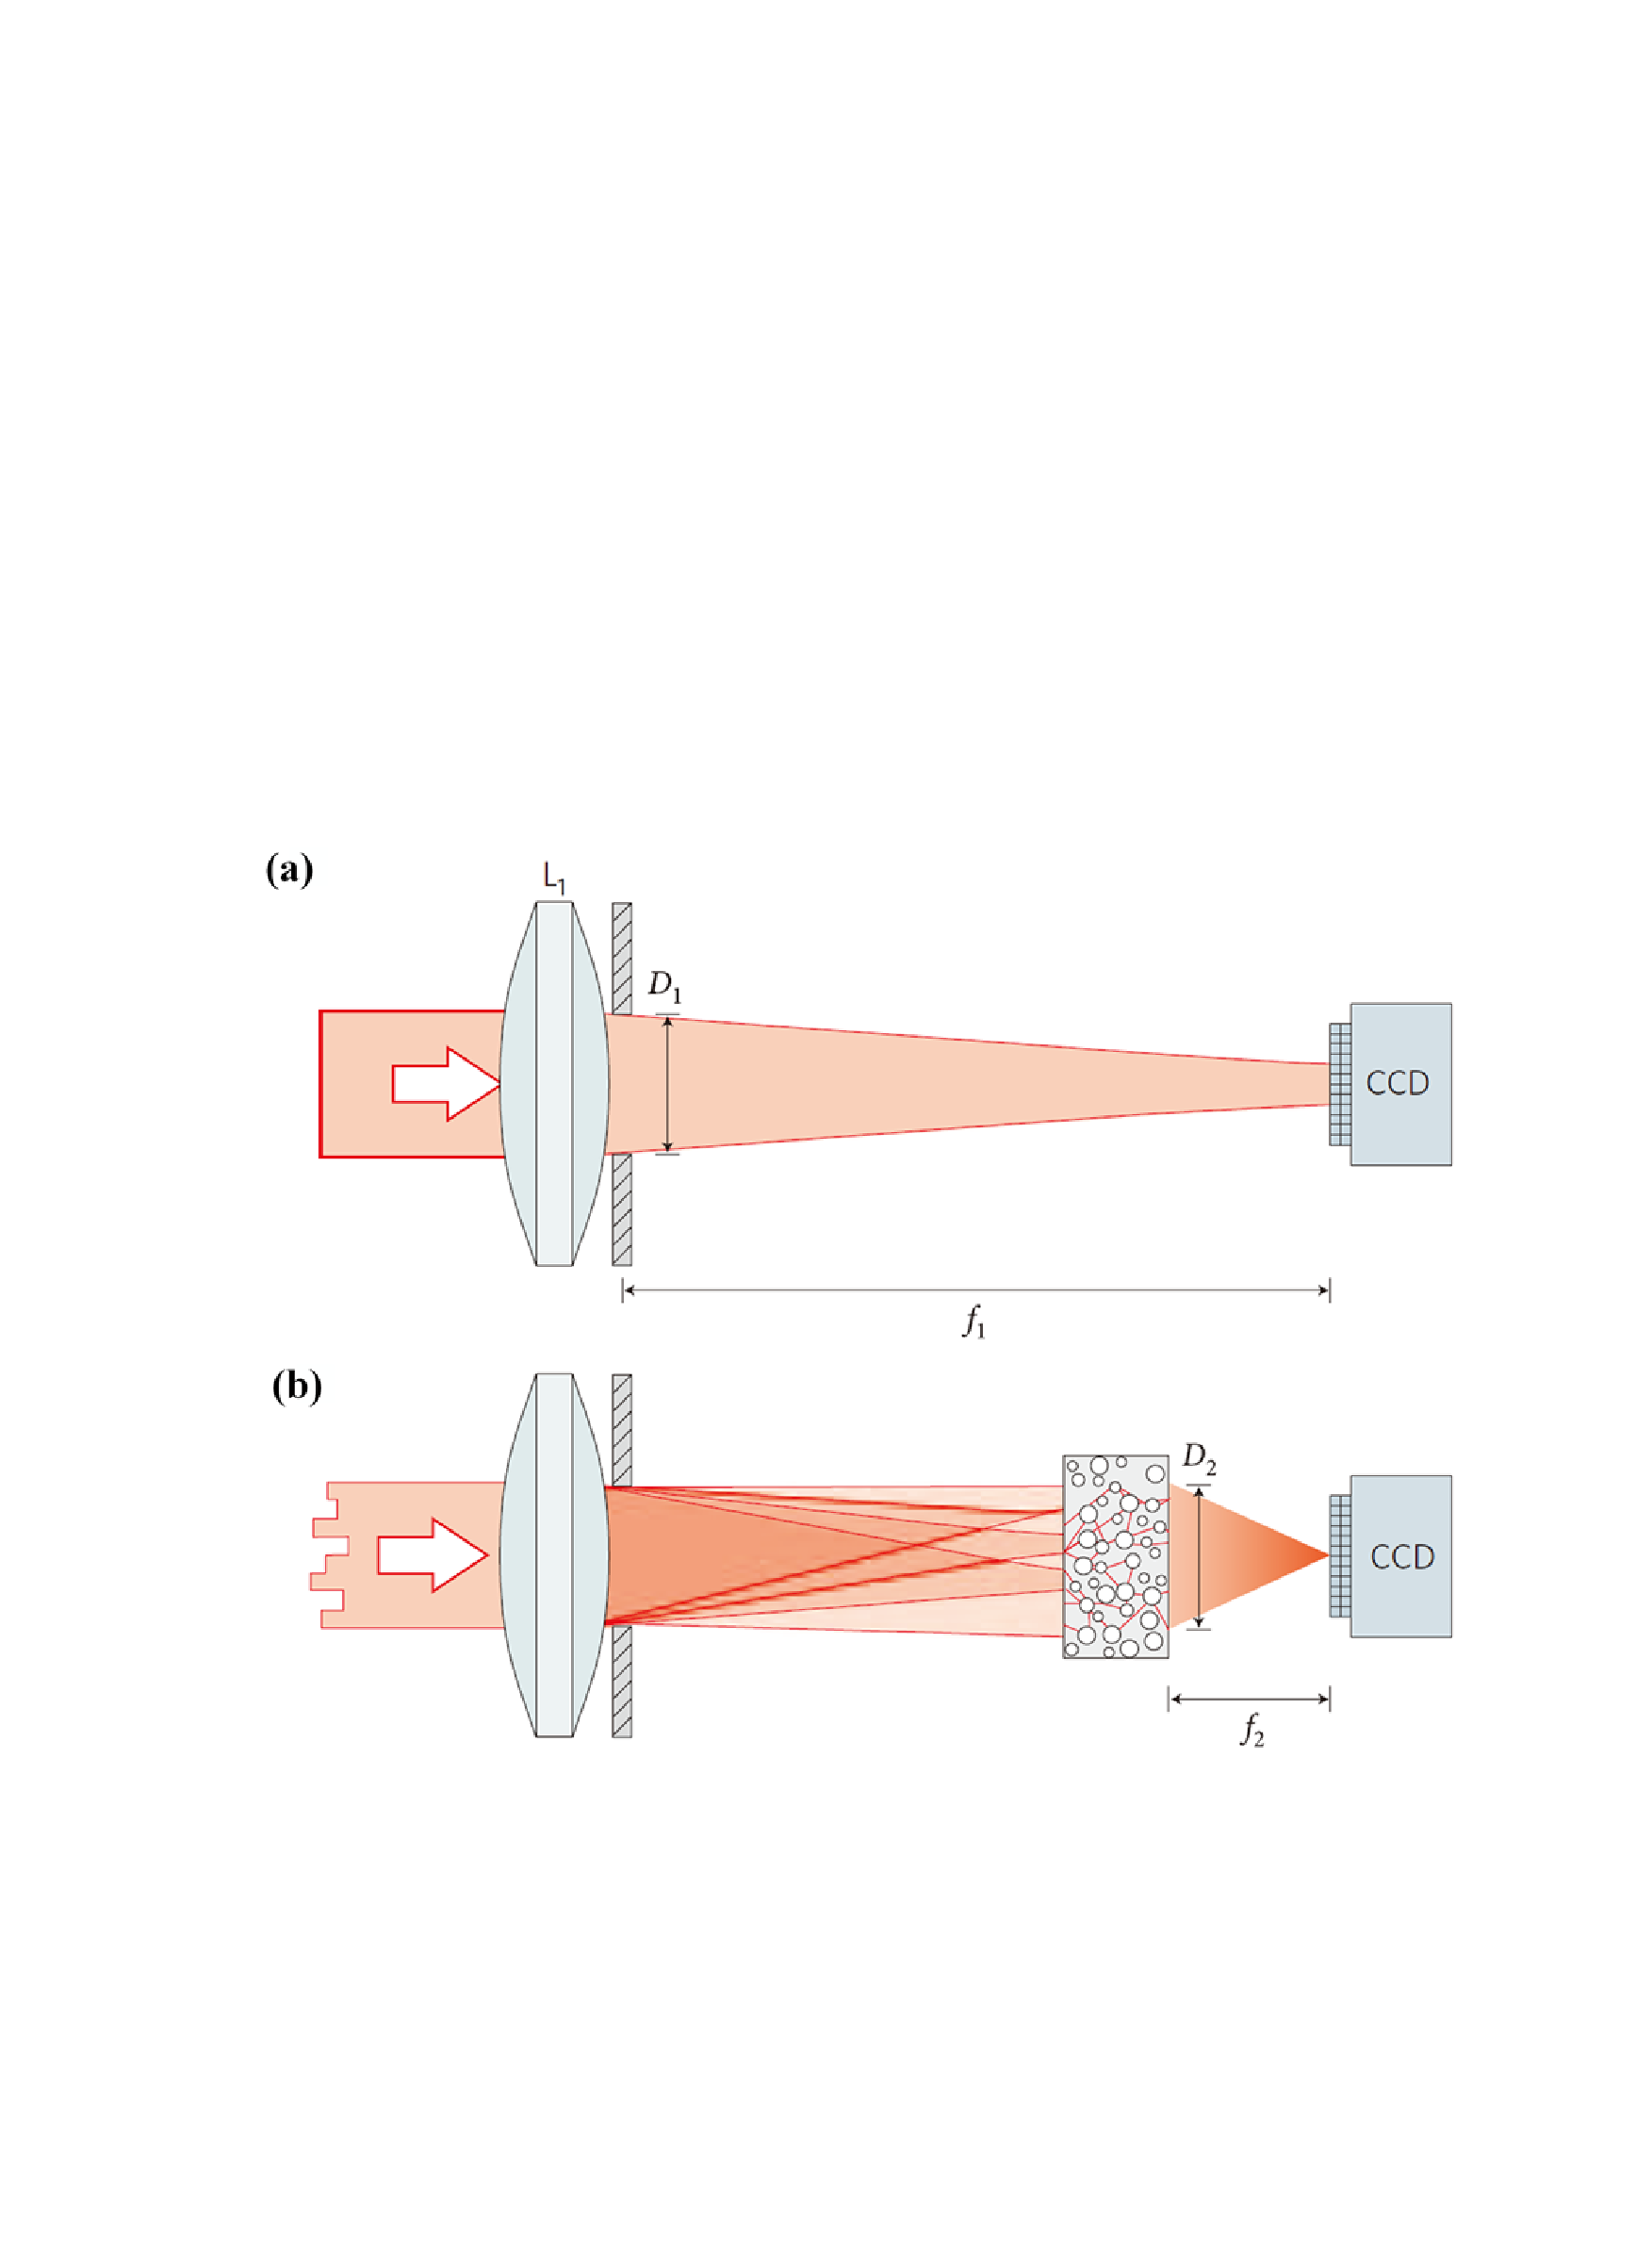
\includegraphics[scale=0.5]{C2.fig4}
	\caption{超衍射极限聚焦示意图}
	\label{fig2:4}
\end{figure}

\begin{figure}[htp]
	\centering
	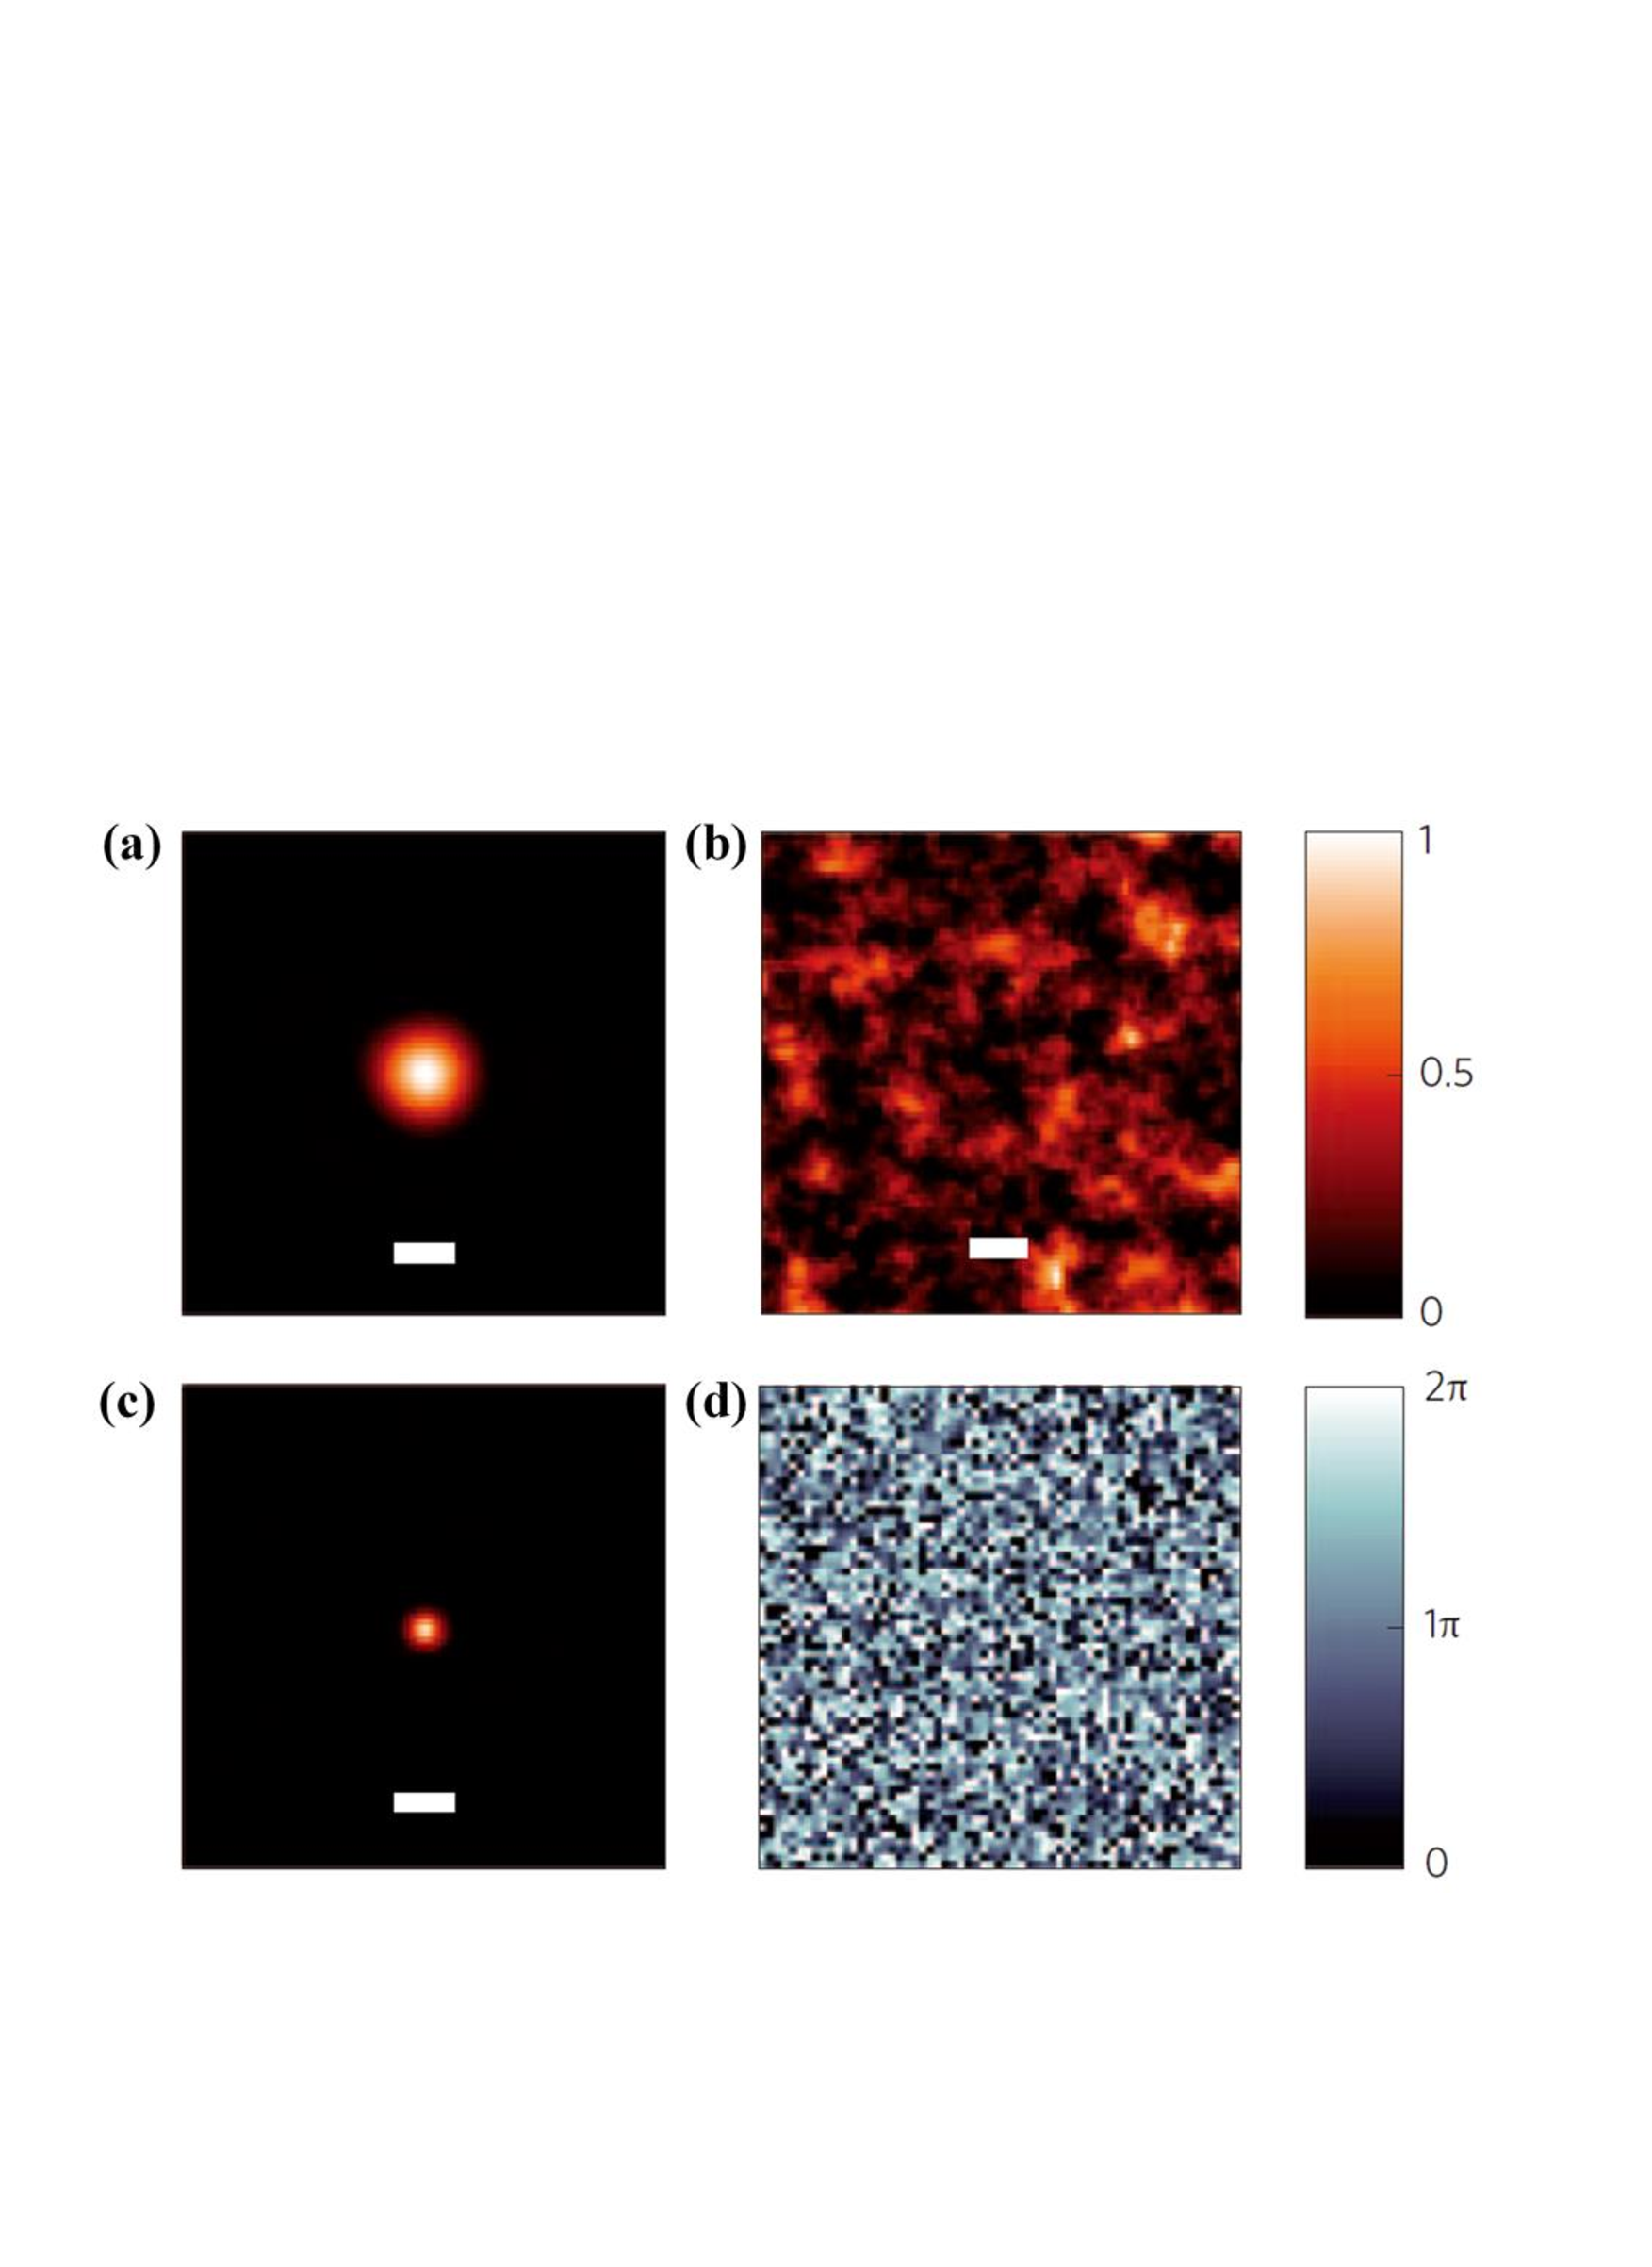
\includegraphics[scale=0.5]{C2.fig5}
	\caption{超衍射极限聚焦实验结果}
	\label{fig2:5}
\end{figure}

2011年,Mosk课题组在利用随机散射介质实现超衍射极限聚焦工作的基础上,提出了一种基于SLM的随机散射透镜超衍射极限扫描显微成像方法。该课题组利用反馈控制调节聚焦的方法将光源聚焦到显微镜的物平面上,调节SLM并扫描整个物平面,实现了对金纳米粒子的观测,分辨率可达97 nm。该方法不需要使用荧光分子对样本进行标记,可以实现对样本的无损观测,实验结果如图\ref{fig2:6}所示,图\ref{fig2:6}(a)为传统显微镜成像;图\ref{fig2:6}(b)超衍射极限成像;图\ref{fig2:6}(c)为图(a)左边第一颗粒子的中心切线与图(b)左边第一颗粒子的中心切线对比。

\begin{figure}[htp]
	\centering
	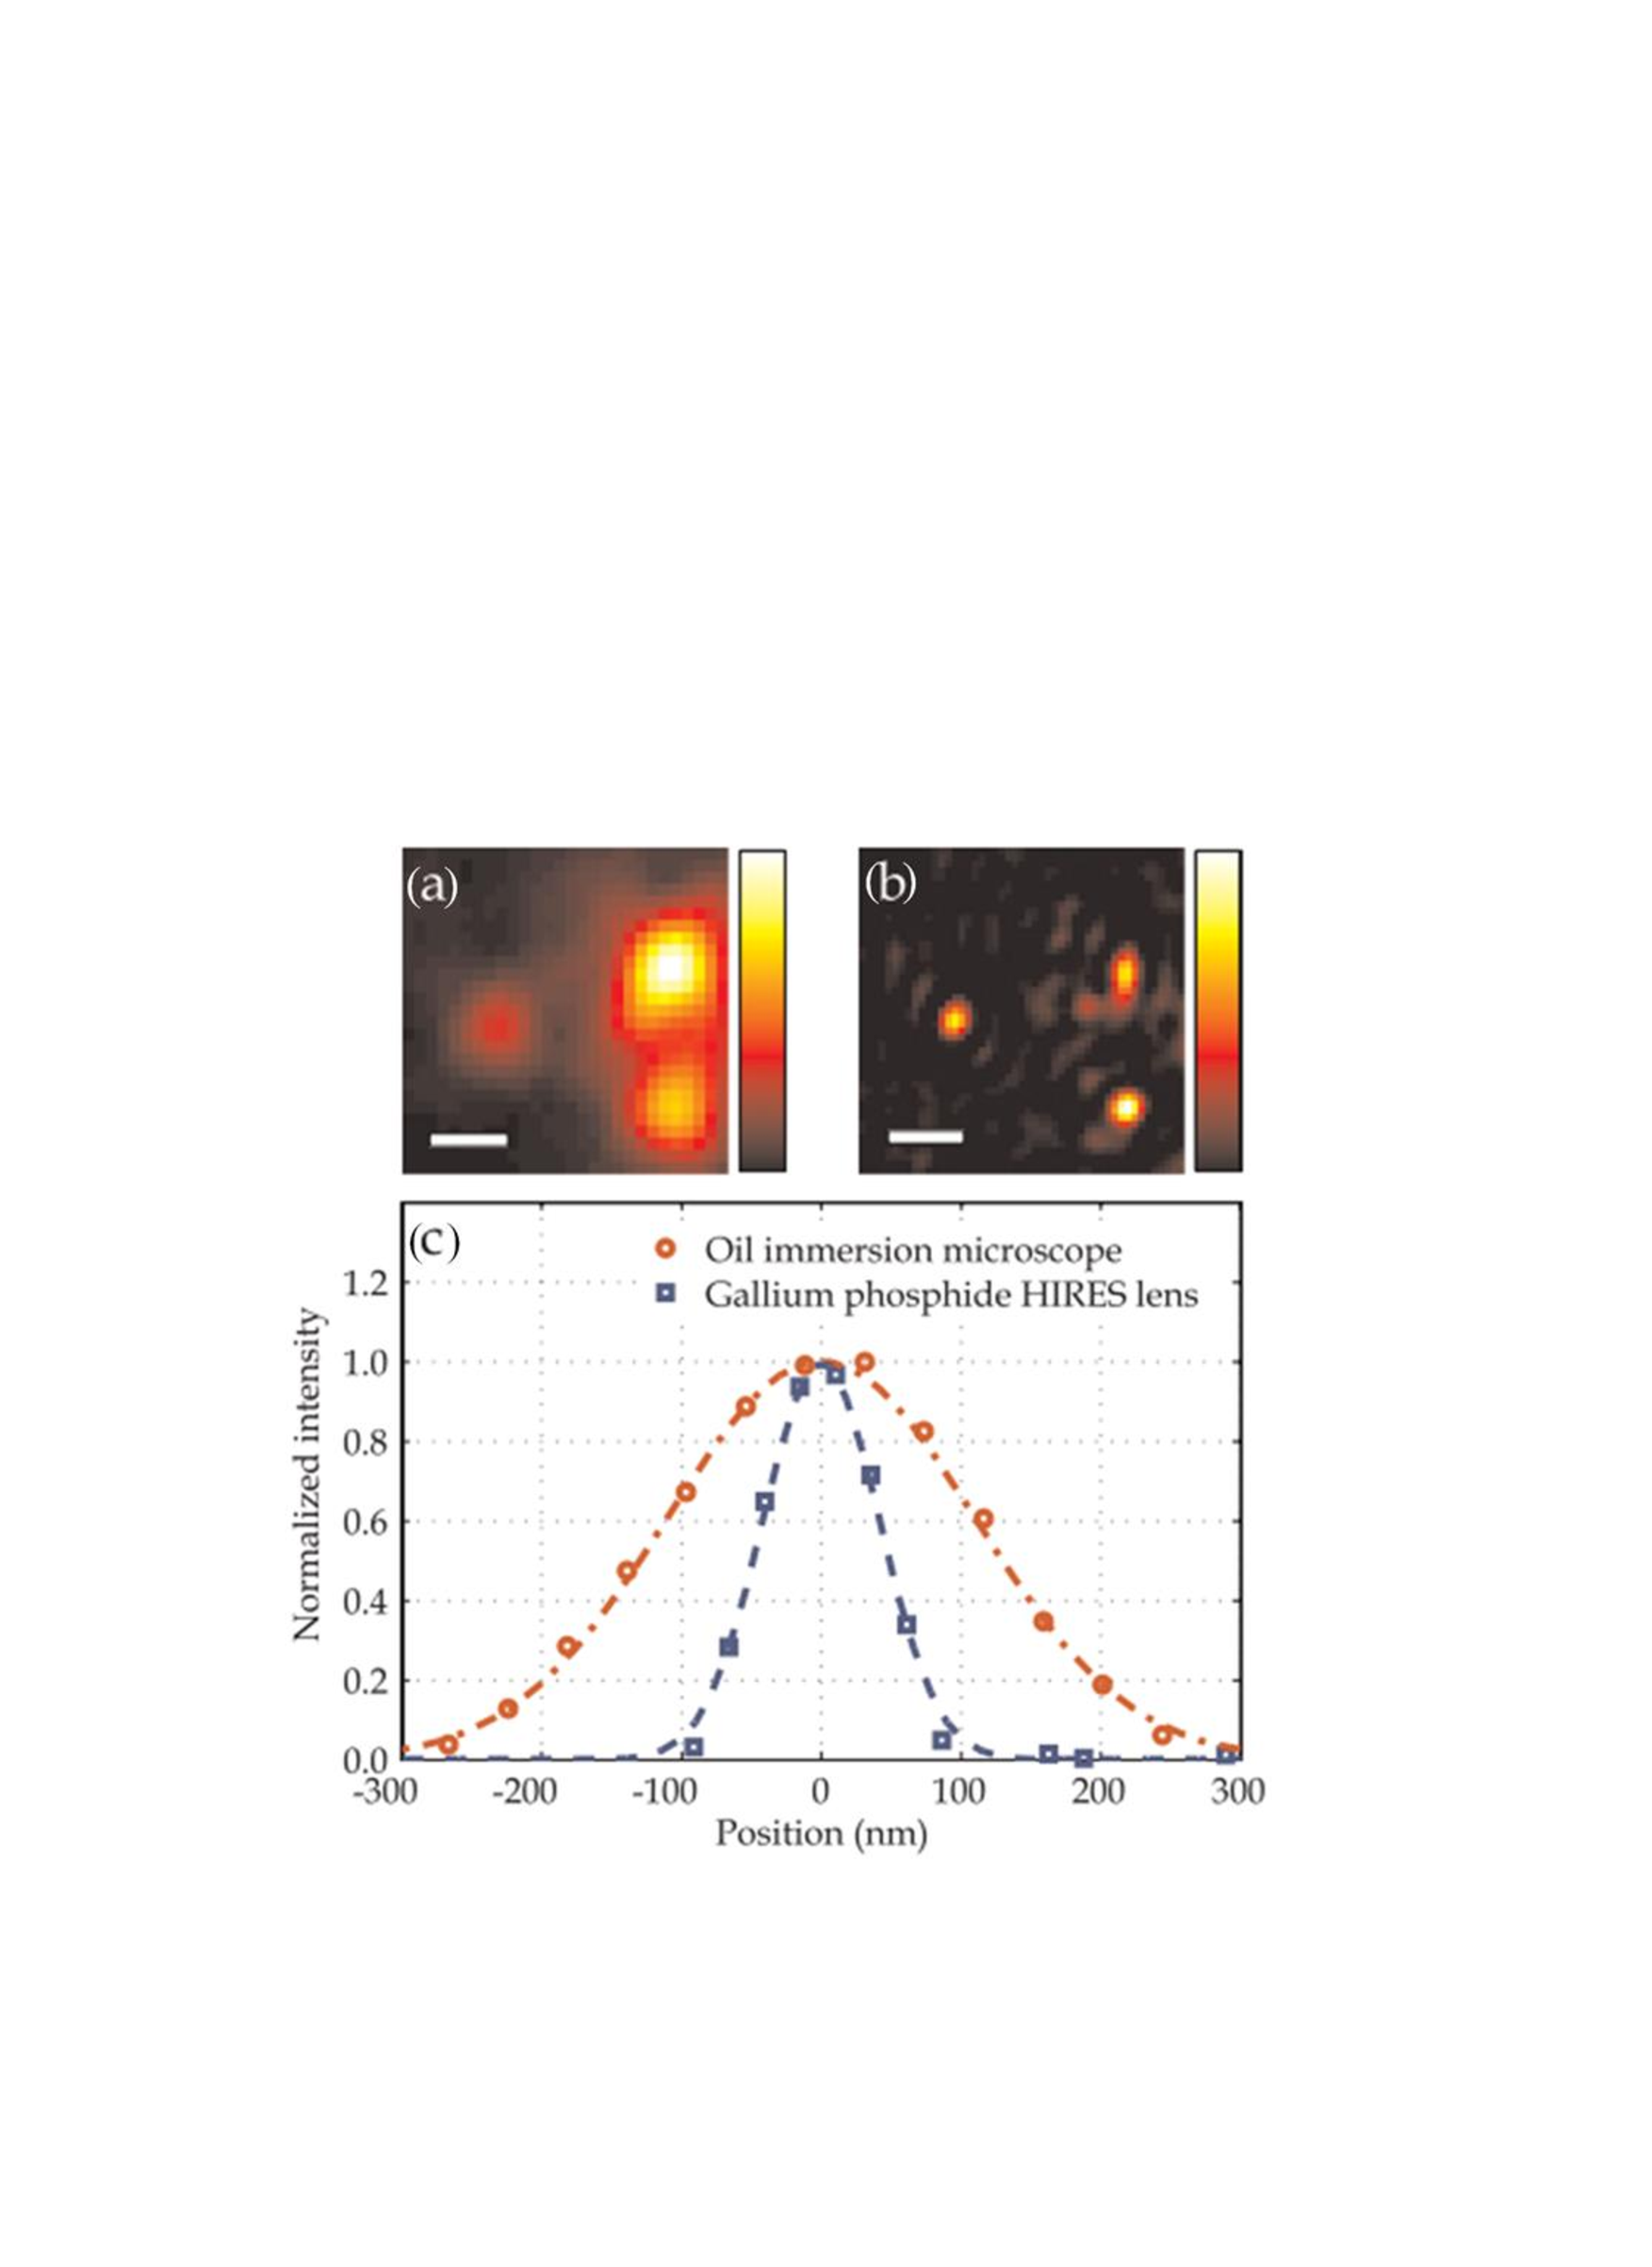
\includegraphics[scale=0.5]{C2.fig6}
	\caption{利用随机散射透镜实现的超衍射极限成像}
	\label{fig2:6}
\end{figure}

时效性是基于反馈优化的波前整形技术的关键问题。为解决这一问题,Cui等人提出了一种空间频率域并行波前优化的方法,该方法可以提升原有反馈控制算法的空间聚焦效率;Conkey等[16]采用全局优化的思想代替原有的逐点优化,通过遗传算法实现了最终的聚焦,得到了更好的聚焦效果;随后,Blochet等将基于MEMS的SLM与现场可编程门阵列(FPGA)技术结合,实现了4 $kHz$左右的调制速度,将该技术应用于波前整形可有效提升成像速度。
值得注意的是,2012年,Katz等人基于反馈优化的波前整形技术,采用非相干光源实现了透过散射介质的实时成像,此项工作极大地推动了波前整形技术在实际应用上的进程。同时,基于反馈优化的波前整形技术在透过多模光纤的光学精密控制和成像方面也有着重要意义。此外,考虑到实际应用中散射介质的时变特性,如何实现透过动态散射介质的快速聚焦或成像是未来研究中的重要课题。

2019年,法国Antoine等人提出了基于散斑方差的非入侵式波前优化方法,利用荧光信号散斑的方差作为波前优化算法的反馈信息,进行散斑信号方差优化,实现了透过散射介质的非入侵波前优化聚焦,此工作大幅推进了波前优化技术在生物医学应用领域的进程。图\ref{fig2:19}所示为基于散斑方差的非入侵式波前优化方法示意图,图\ref{fig2:20}为基于散斑方差的非入侵式波前优化聚焦结果。在图\ref{fig2:20}中,图\ref{fig2:20}(a)为散斑信号;图\ref{fig2:20}(b-d)为不同随机初始优化后聚焦结果;图\ref{fig2:20}(e)为不同随机初始散斑的方差曲线图;图\ref{fig2:20}(f-h)分别为散斑总强度曲线图、散斑对比度曲线图和散斑中心区域对比度曲线图。

\begin{figure}[htp]
	\centering
	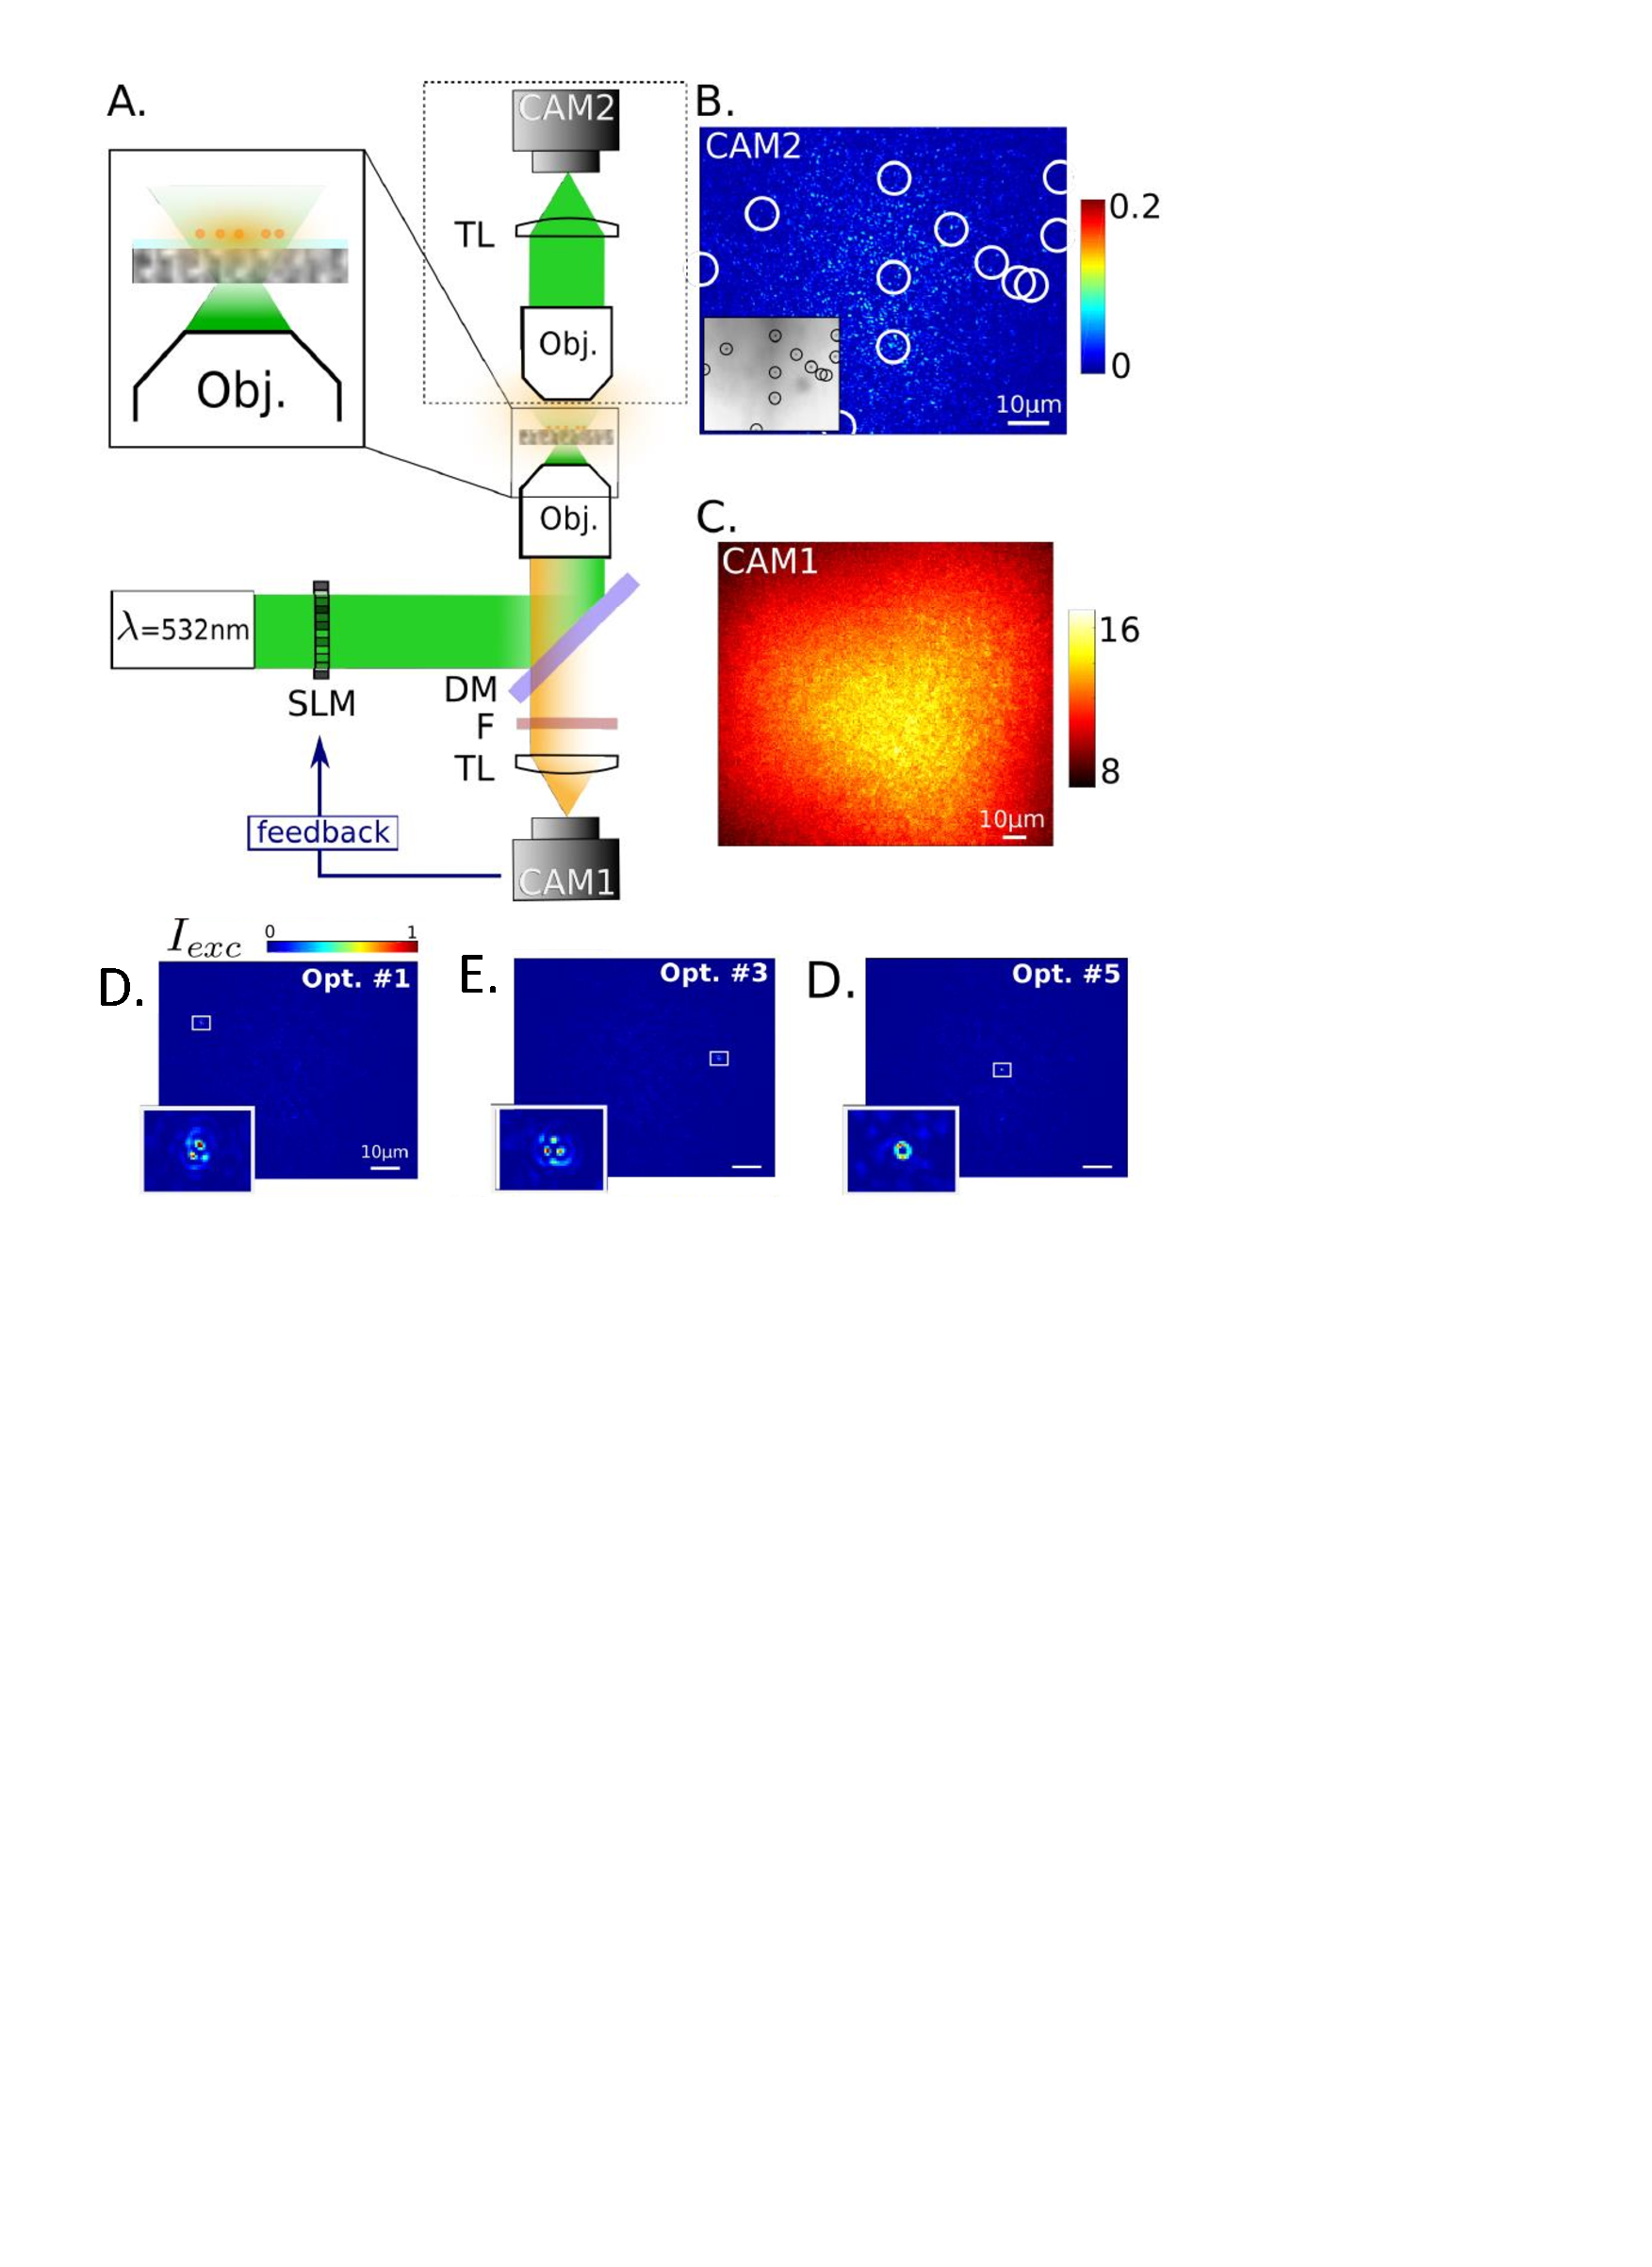
\includegraphics[scale=0.50]{C2.fig19}
	\caption{基于散斑方差的非入侵式波前优化方法示意图}
	\label{fig2:19}
\end{figure}

\begin{figure}[htp]
	\centering
	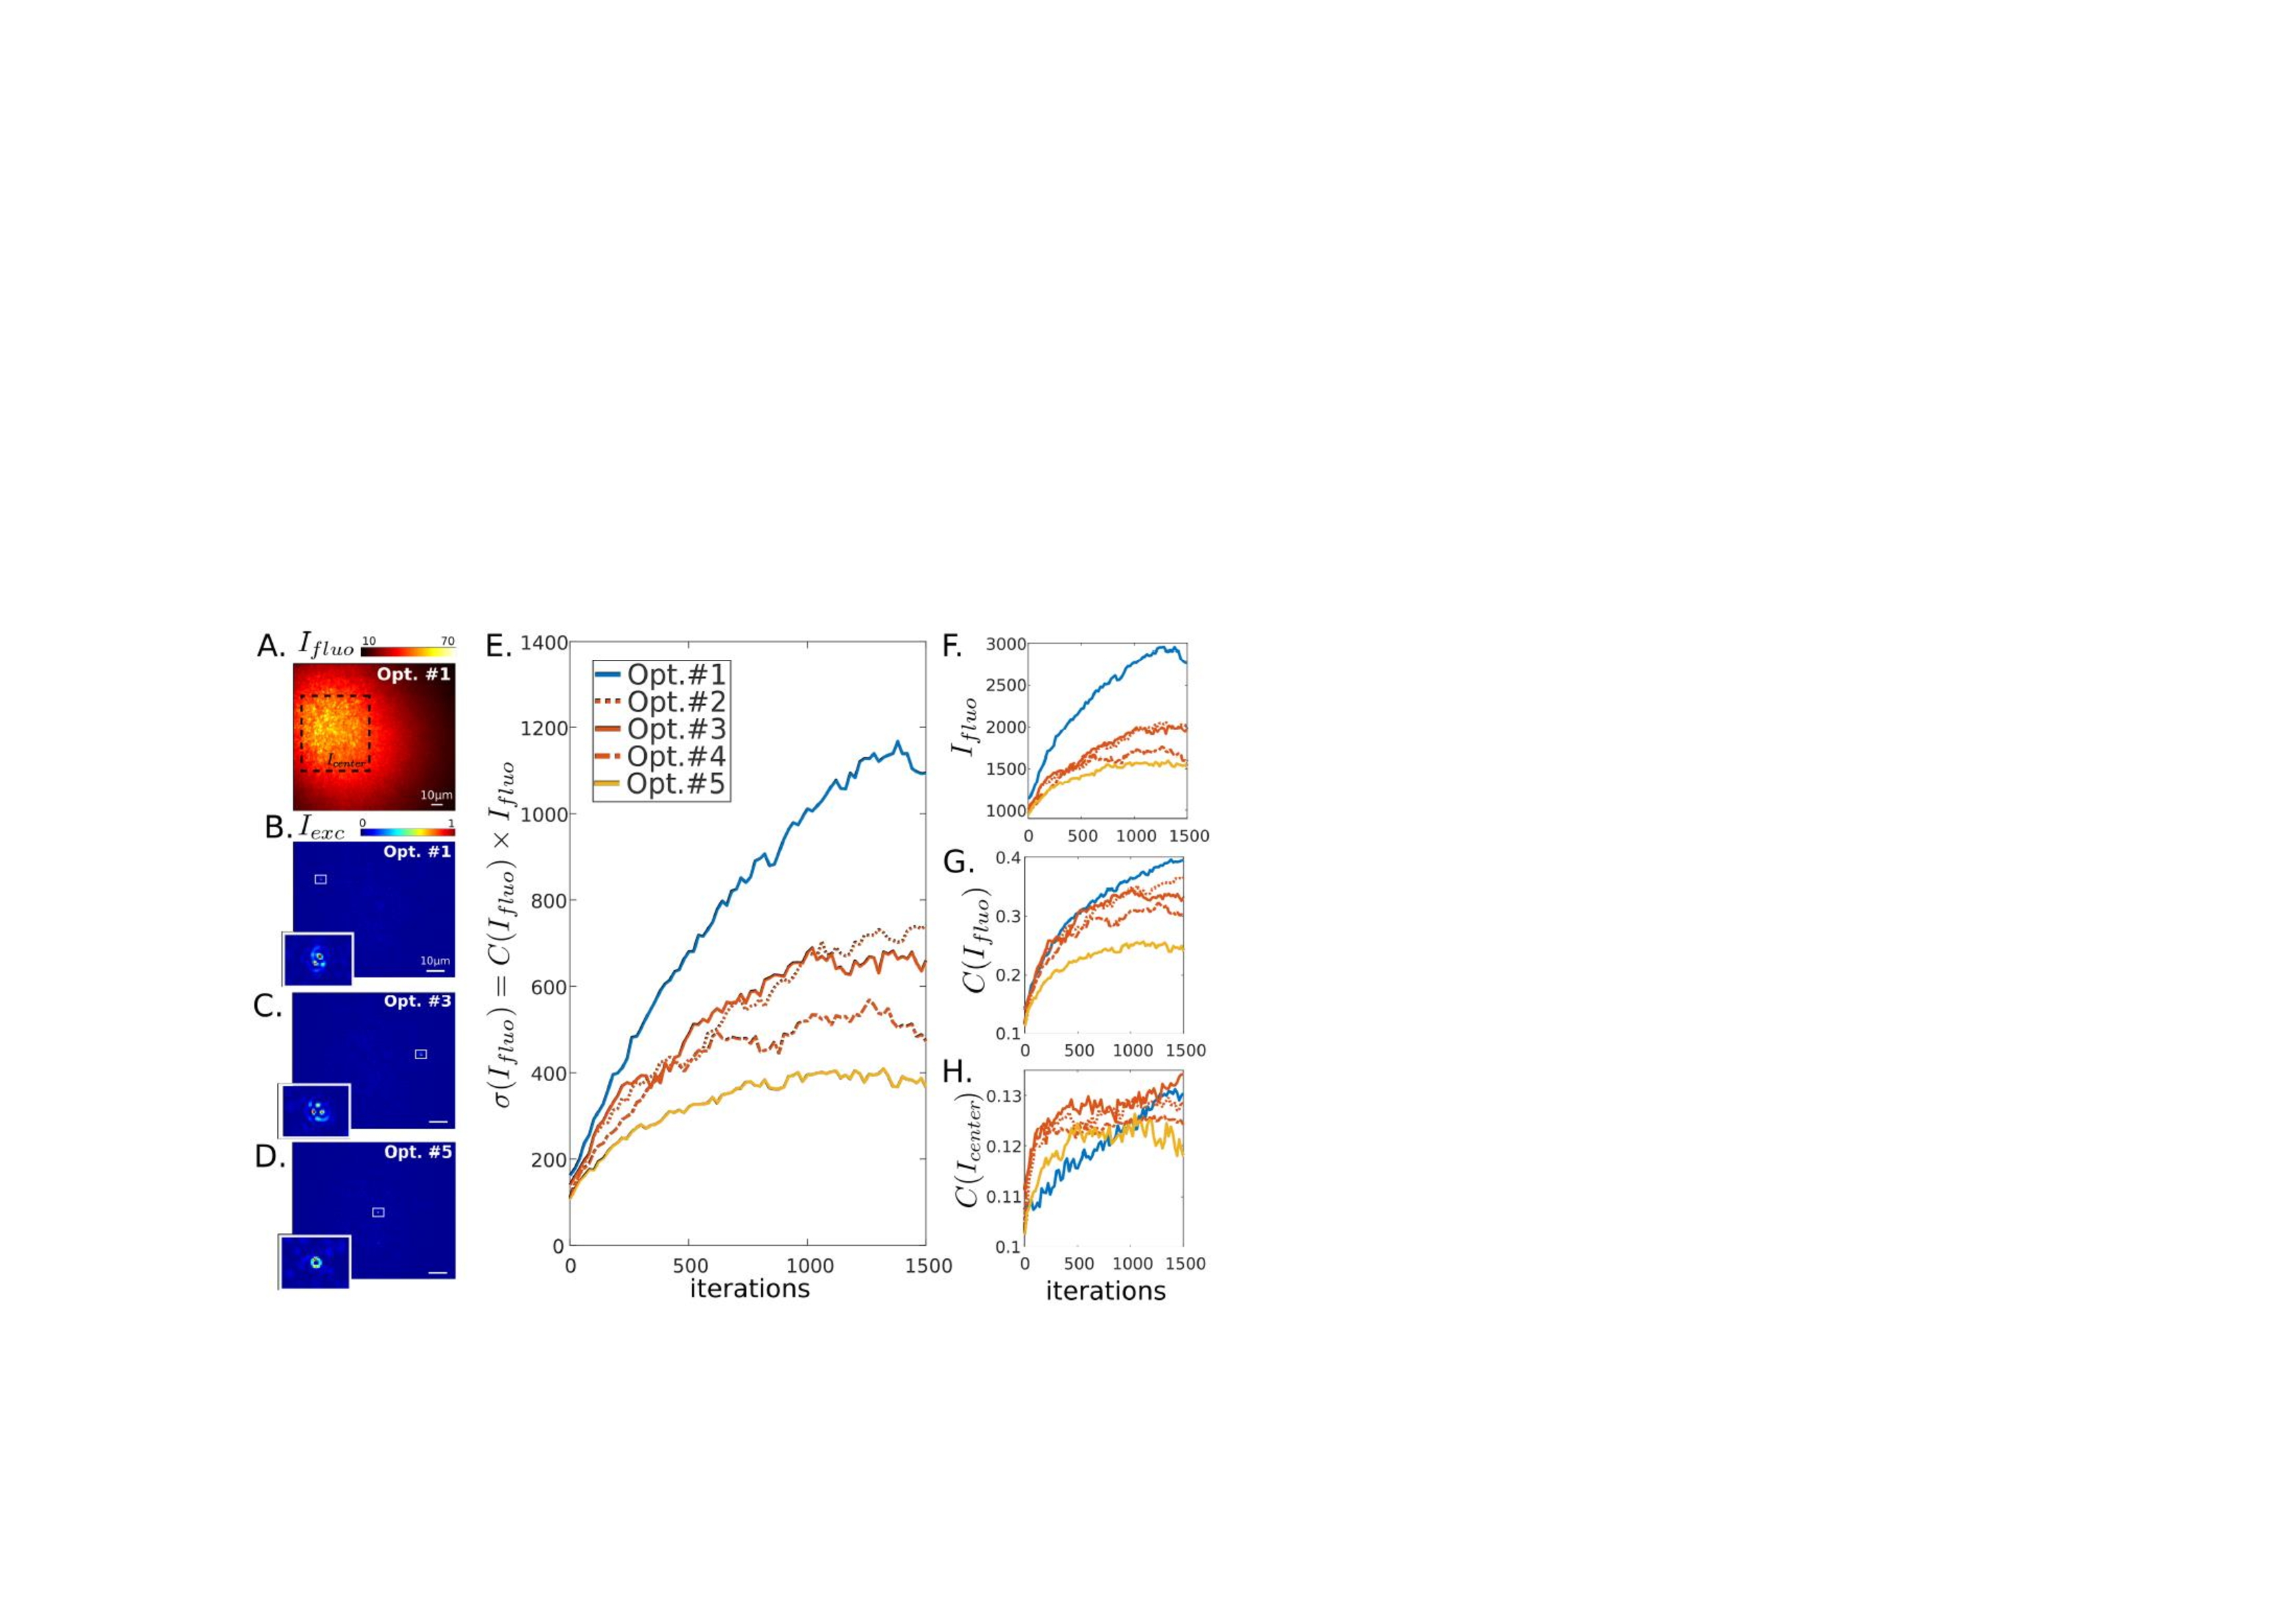
\includegraphics[scale=0.50]{C2.fig20}
	\caption{基于散斑方差的非入侵式波前优化聚焦结果}
	\label{fig2:20}
\end{figure}

\subsection{光学传输矩阵的散射介质成像技术}

在Mosk等利用波前调制技术验证了可见光透过散射介质后依然能够实现聚焦之后,基于波前调制技术的相关研究引起了世界各国科研人员的广泛关注。测量传输矩阵是一种新的波前调制技术,该方法的核心思想是利用一个复杂的矩阵将入射光场与出射光场联系起来,通过测量传输矩阵并结合相位共轭技术,能够在任意位置、任意时刻实现聚焦和成像。

假设光源是线性极化的,则对于光波在任何介质中的传播过程,都可以用格林函数进行描述。离散化的格林函数可以表征介质对入射光波的作用,离散化的格林函数就是上述提到的光学传输矩阵,它表示$m$个输出单元与$n$个输入单元的光场信息(振幅和相位)之间的相互关系,可以表示为:

\begin{equation}
    E_{m}^{out}=\sum_{n}^{N}k_{mn}E_{m}^{in}
\label{eq:2.1}
\end{equation}
式中,$E_{m}^{in}$表示输入光场信息;$E_{m}^{out}$表示输出光场信息;$k_{mn}$表示光学传输矩阵的元素;$N$为光场调制模式总数。

在测得光学传输矩阵$K$后,假设目标输出光场为$E_{m}^{target}$,利用相位共轭技术可以估计出输入光场,即

\begin{equation}
    E_{cal}^{in}=K^{\dag} \cdot E_{target}^{out}
\label{eq:2.2}
\end{equation}
式中:$E_{cal}^{in}$表示计算得到的输入光场;$^{\dag}$表示取共轭。则实际输出光场$E^{out}$可以表示为
\begin{equation}
  E^{out}=K \cdot E_{cal}^{in} =K \cdot K^{\dag} \cdot E_{target}^{out}
\label{eq:2.3}
\end{equation}
由以上分析可知,一旦测得散射介质的光学传输矩阵,就可以采用相位共轭的方法实现聚焦。

2010年,法国卡斯特勒-布罗塞尔实验室(Laboratoire Kastler-Brossel)的Popoff等人利用四步相移干涉法测得了ZnO散射介质的光学传输矩阵,图\ref{fig2:7}所示为该实验的测量原理。

\begin{figure}[htp]
	\centering
	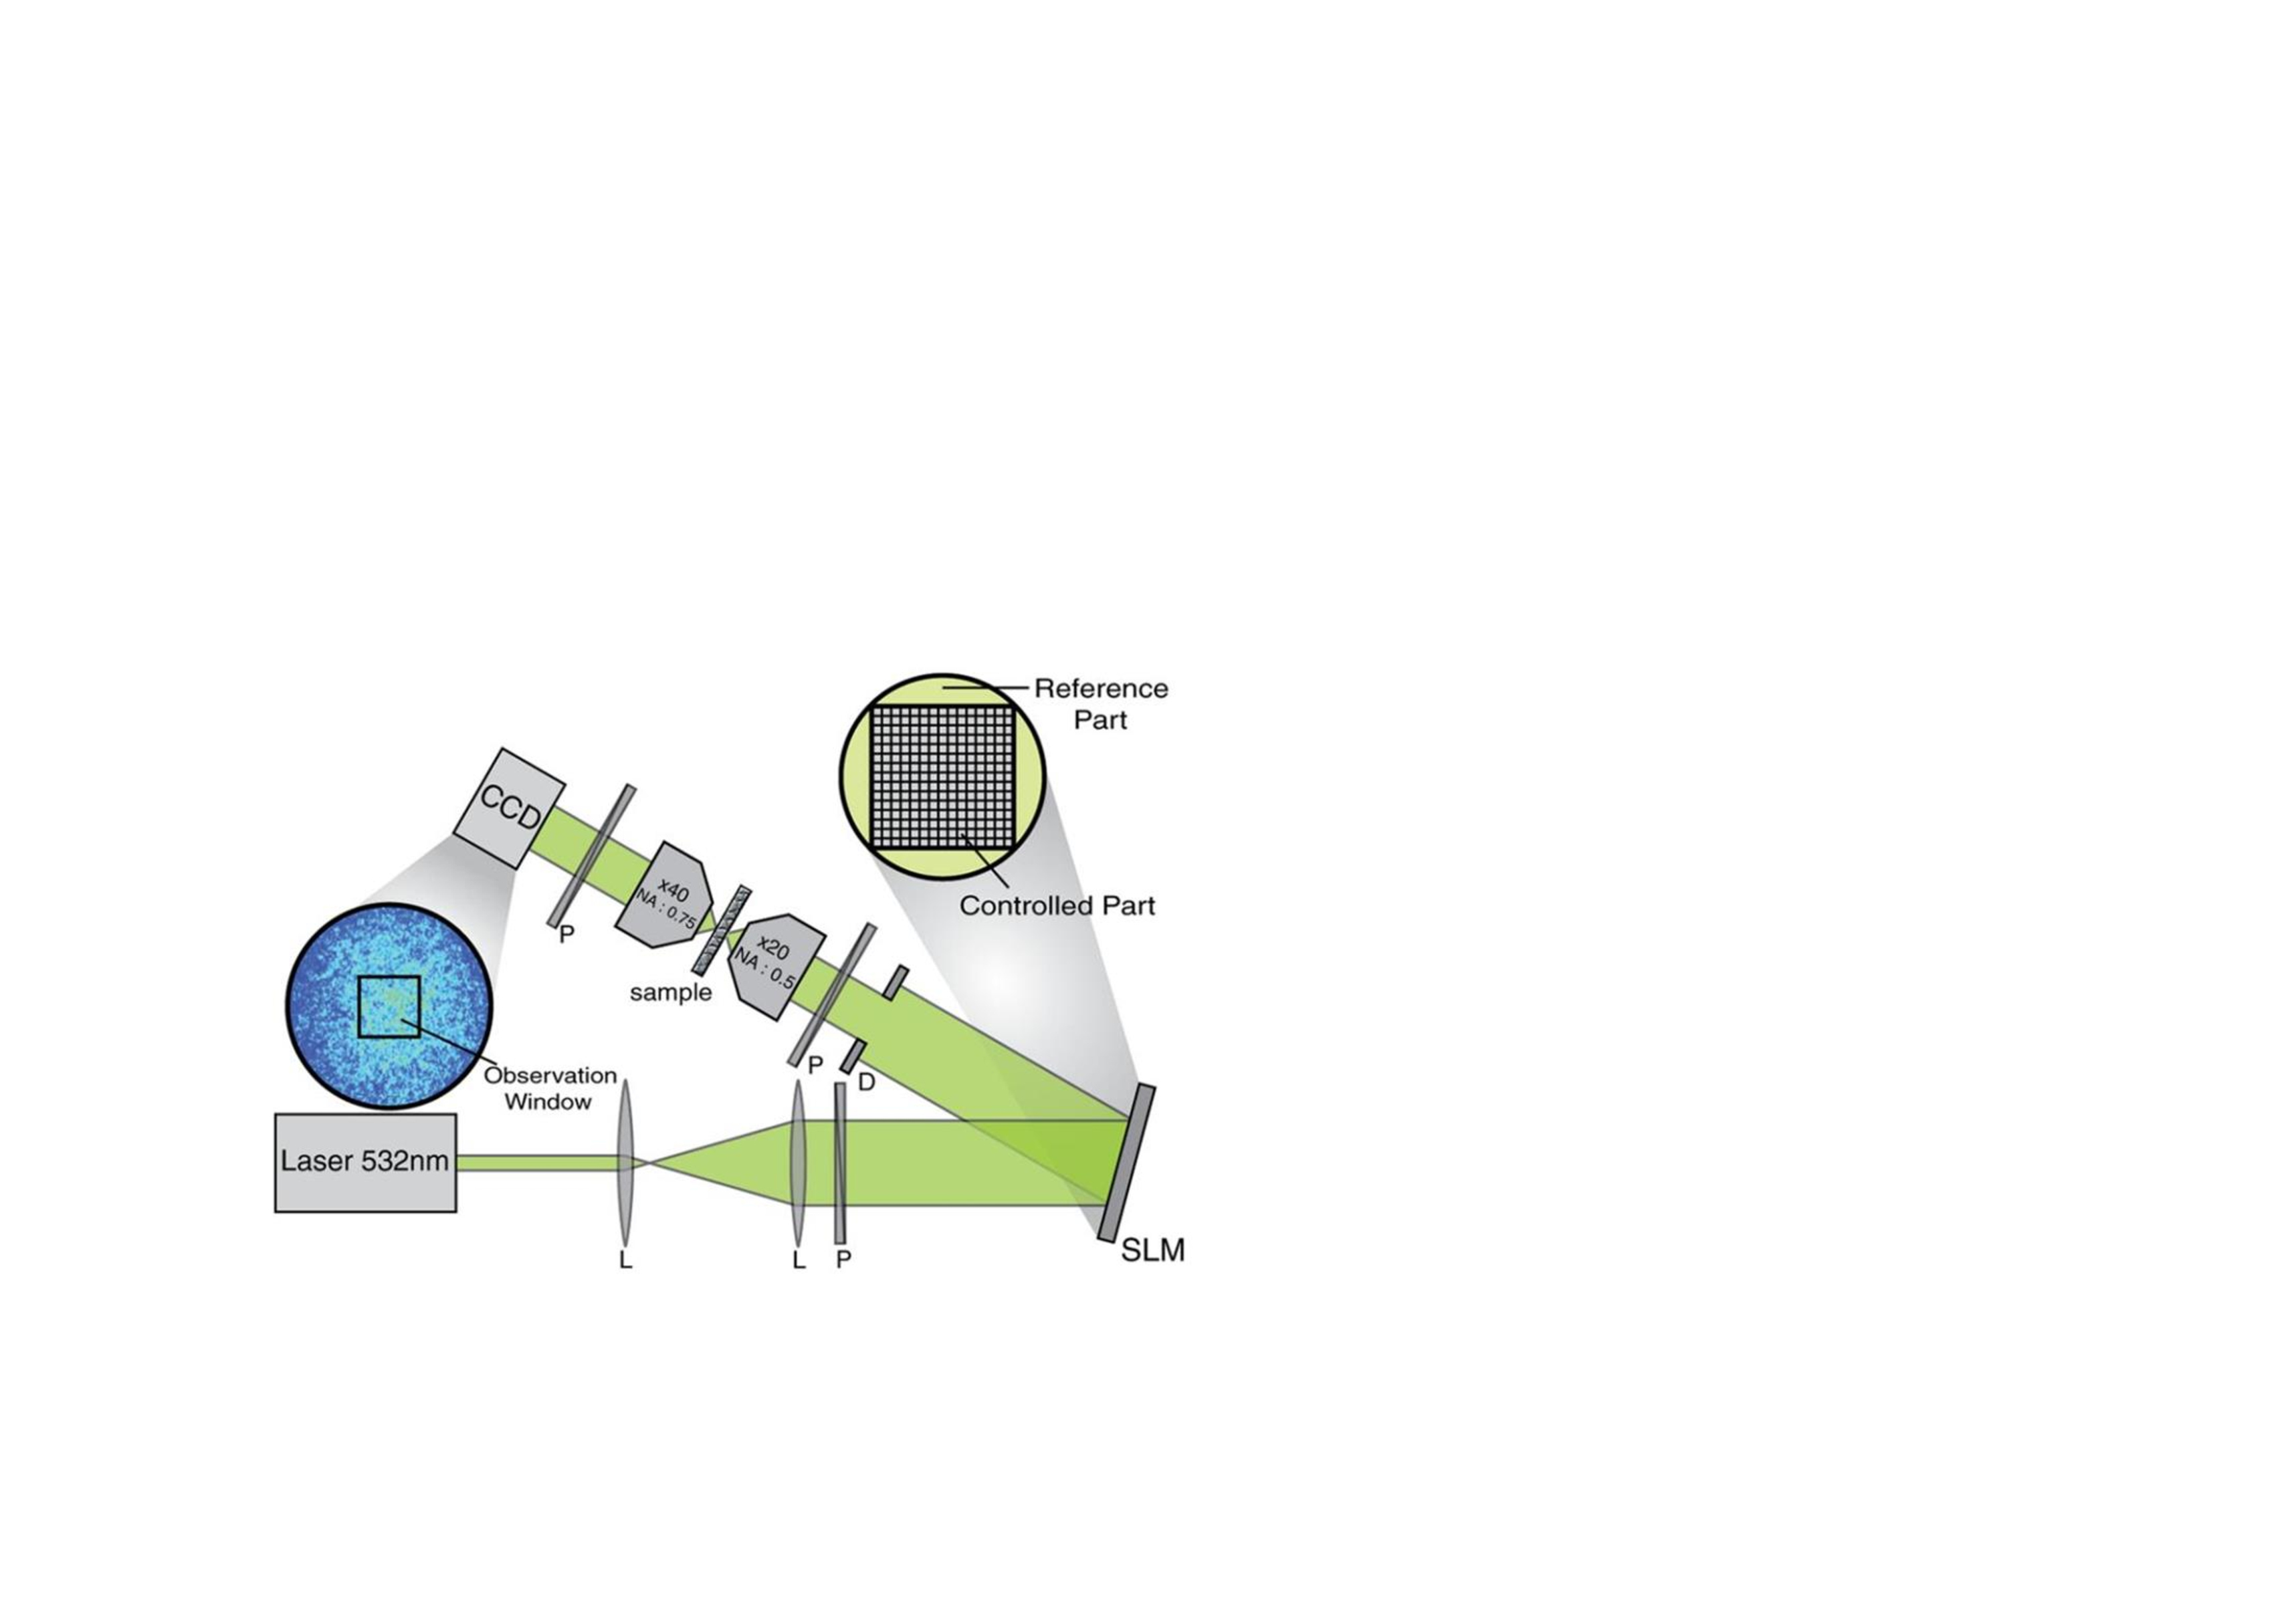
\includegraphics[scale=0.5]{C2.fig7}
	\caption{四步相移测量传输矩阵的实验原理图}
	\label{fig2:7}
\end{figure}

在测得ZnO介质的传输矩阵后,Popoff等人利用Tikhonov正则化图像恢复算法对散斑进行了重建,实验结果如图\ref{fig2:8}所示,图\ref{fig2:8}(a)为聚焦前散斑;图\ref{fig2:8}(b)为单点聚焦结果;图\ref{fig2:8}(c)为多点聚焦结果。在重建图像时,除了相位共轭方法,往往还需要借助Thiknov、Total Variation复原等优化算法来获得更高质量的重建图像,因此研究不同重建算法的优劣具有重要意义。

\begin{figure}[htp]
	\centering
	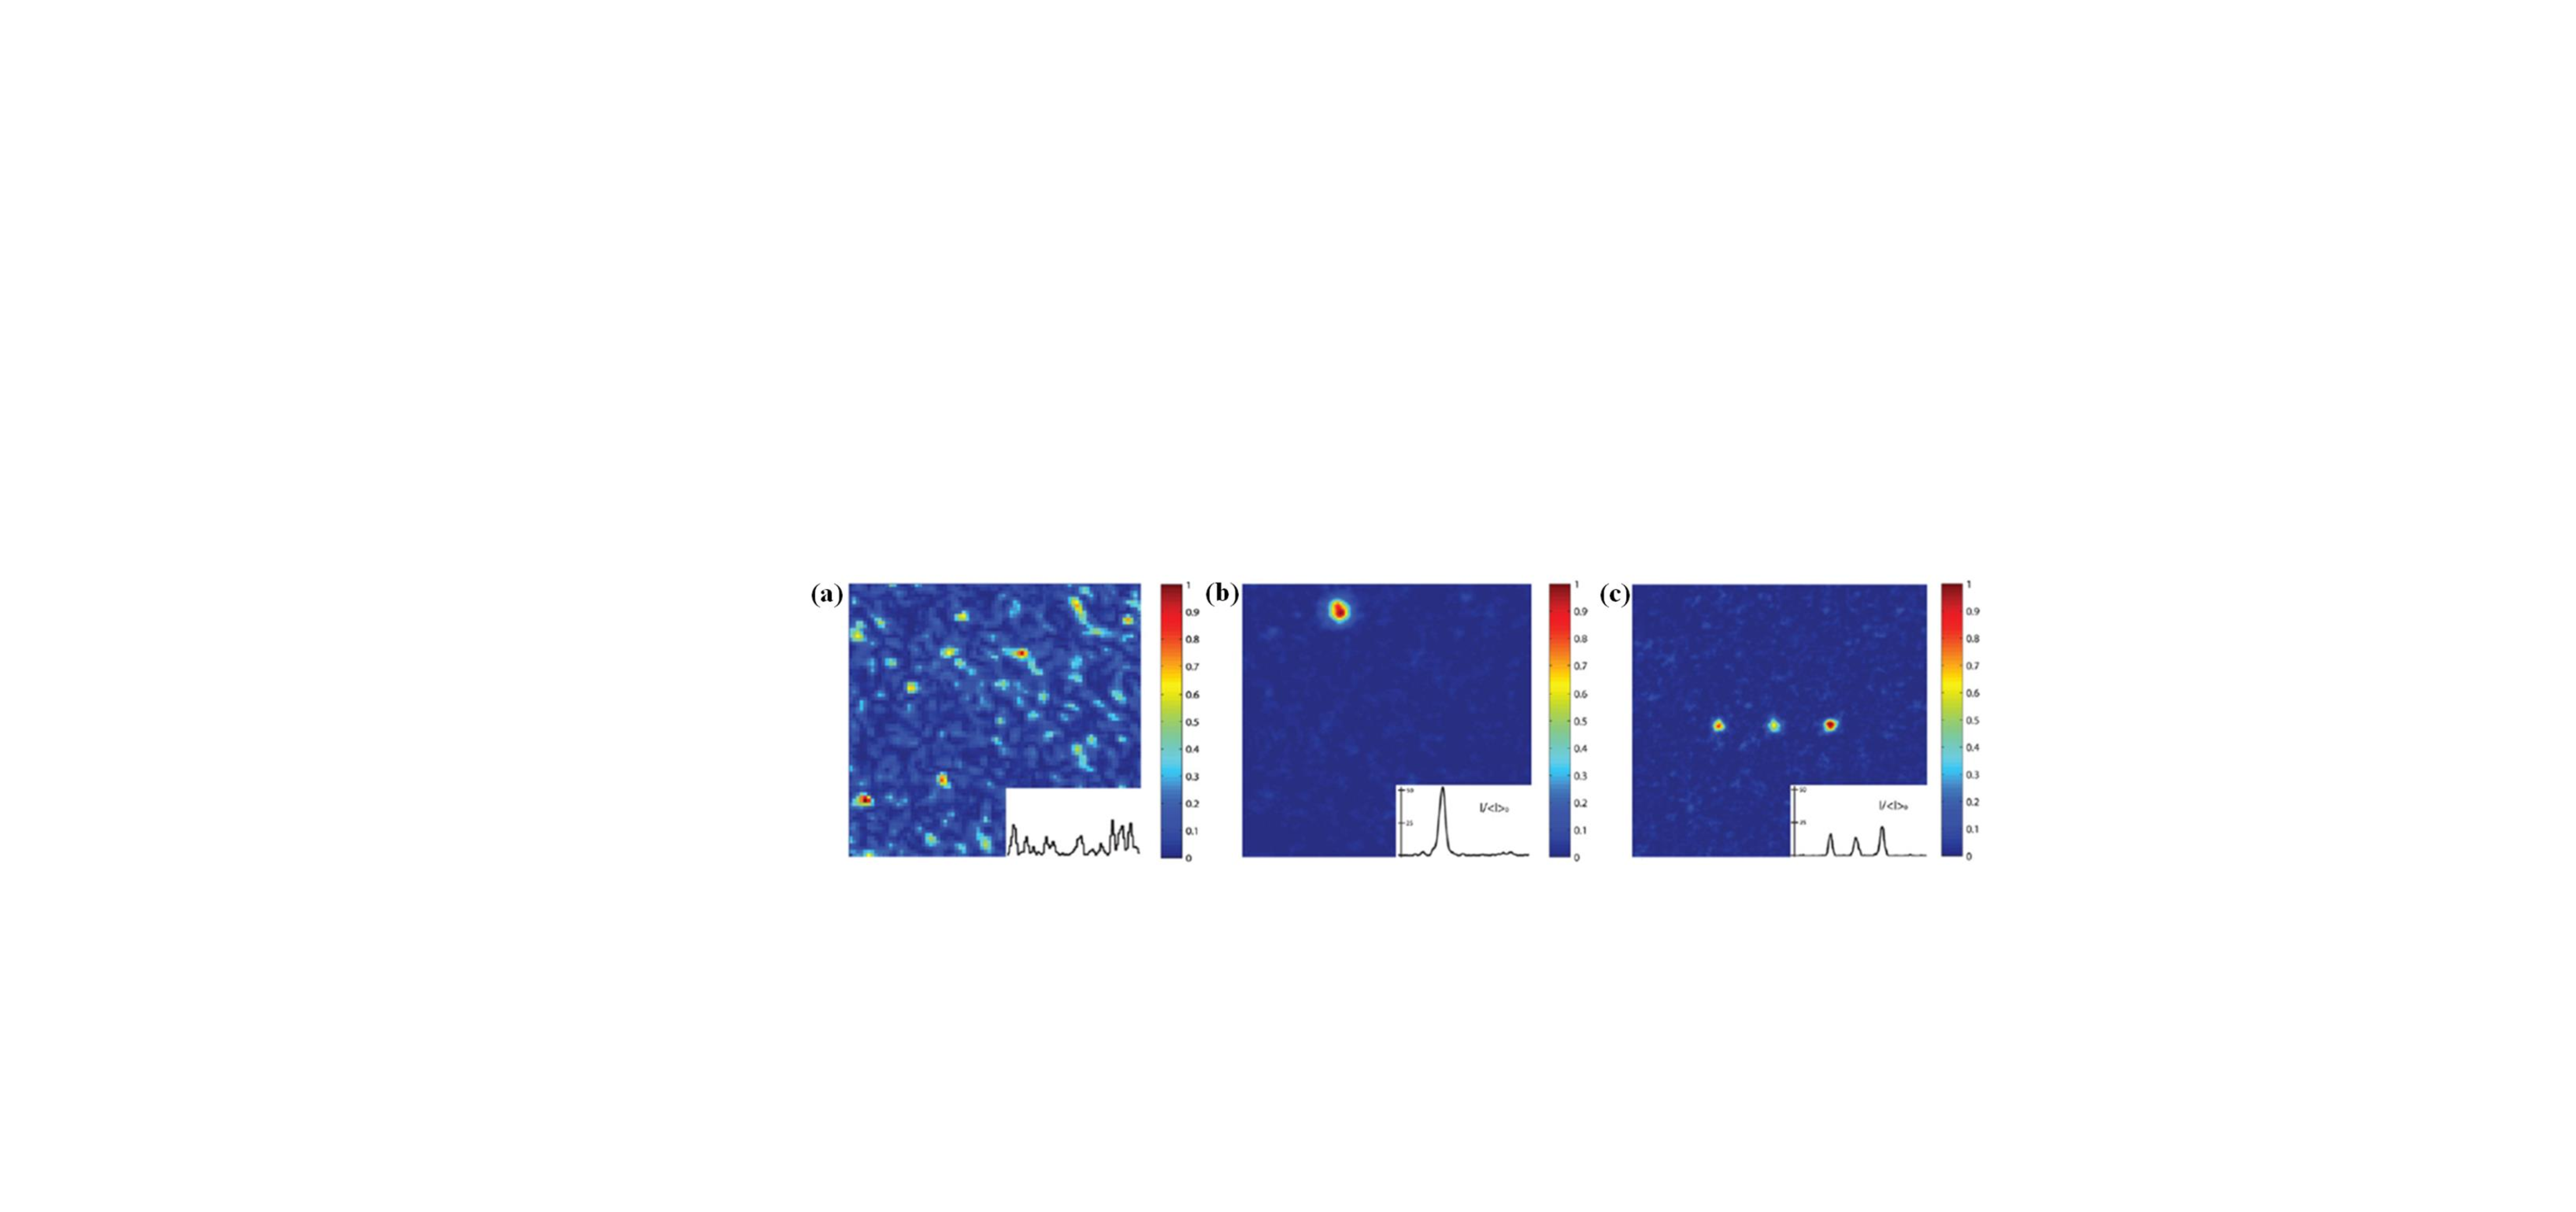
\includegraphics[scale=0.35]{C2.fig8}
	\caption{采用相位共轭法得到的聚焦结果}
	\label{fig2:8}
\end{figure}

基于光学传输矩阵的散射成像方法的优点在于只要测量出成像系统的光学传输矩阵,便可以从任意目标所成的散斑中迅速恢复出待测目标。但是,就现阶段的研究来看,该方法所需系统较复杂,对系统稳定性的要求非常高,任何改变都有可能导致无法重建目标,目前的研究水平还无法做到对实际物体成像。

虽然光学传输矩阵方法已在实验中得到了验证,但是在实际应用中仍有许多不足之处。随着对光学传输矩阵方法研究的深入,许多光学传输矩阵测量方法被提了出来,如:2011年Choi等提出的频域传输矩阵测量方法、2015年Drémeau等提出的基于相位恢复算法的测量方法、2015年Yoon等提出的基于波前相位调制的测量方法。不同的测量方法具有不同的特点,如:频域测量方法无法对倏逝波矩阵进行测量,基于相位恢复算法的测量方法的稳定性差,而基于波前调制的测量方法的精确程度受限于调制光的精准程度。2012年,Tripathi等提出了一种测量矢量光学传输矩阵的方法,利用该方法可以获得指定偏振态的聚焦光波;2015年,Andreoli等提出了一种基于测量多光谱传输矩阵的方法,该方法可以实现宽光谱聚焦;2016年,Mounaix等利用多光谱传输矩阵方法实现了控制超短脉冲激光通过散射介质的空时聚焦;在多光谱传输矩阵研究的基础上,2019年Dong等利用多路复用相位反演的光谱方法实现了透过散射介质聚焦。多物理量探测有助于信号的探测和识别,增加光学传输矩阵的测量维度(光谱和偏振)等将在未来的实际应用中起到至关重要的作用。另外,如何保证光学传输矩阵测量的实时性是未来研究的重要方向。

\subsection{非入侵传输矩阵测量技术}

2020年,法国研究人员Antoine等人首次提出了非入侵光学传输矩阵测量技术,实现了完全非入侵条件下实现光学传输矩阵测量并聚焦成像。该工作极大的拓展了光学传输矩阵测量应用场景,利用随机散斑进行着照明,并记录荧光目标所激发的荧光散斑图案,非入侵的方式恢复了照明部分至荧光目标部分输入矩阵,并成功恢复荧光目标至探测器部分输出矩阵,其基本工作原理如图\ref{fig2:23}所示。该工作在一定程度上证明光学传输矩阵方法在实际应用场景中的重要价值。

\begin{figure}[htp]
	\centering
	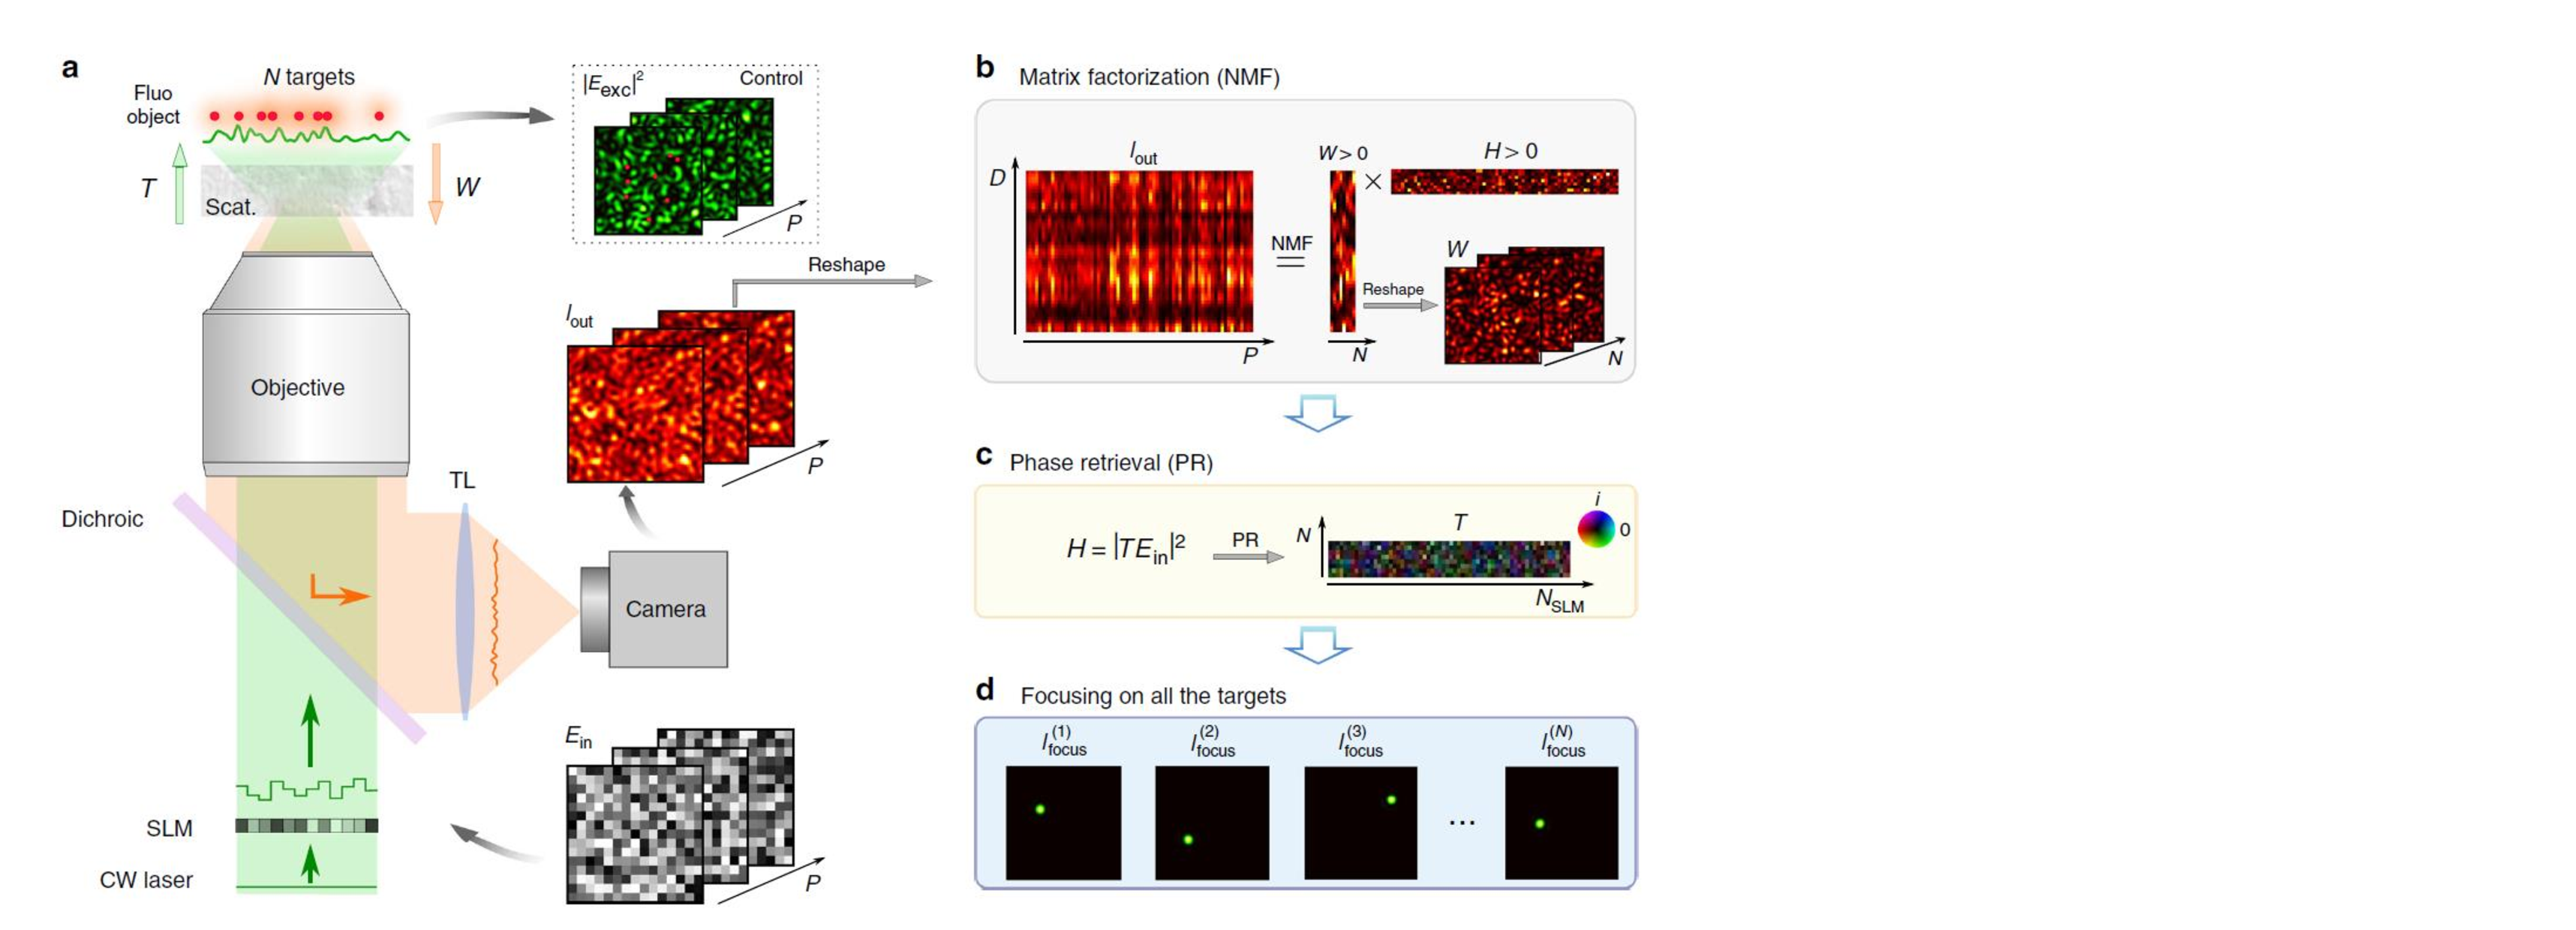
\includegraphics[scale=0.38]{C2.fig23}
	\caption{基于荧光信号的非入侵光学传输矩阵测量原理}
	\label{fig2:23}
\end{figure}


\section{基于光学记忆效应的散射成像技术}

基于光学记忆效应的散射成像技术是透过散射介质成像的重要组成部分,它可以利用散斑,通过自相关运算,获取目标信息的傅里叶振幅,进而结合有效的相位恢复算法实现目标的重建。与波前整形技术相比,基于光学记忆效应的散射成像技术具有非入侵的特点,且对于光源、介质和系统的要求较低。随着对光学记忆效应研究的深入,利用散射介质的退相关特性,可实现透过散射的光谱成像和三维成像,这将对未来的新型成像系统具有重要意义。

\subsection{光学记忆效应}

在一定的入射角度范围内,当改变光源入射方向时,经过散射介质在像平面上得到的散斑形状特征保持不变,但整体发生了平移,这一现象称为光学记忆效应。图\ref{fig2:9}所示为Freund等\cite{Freund1988}所做的关于光学记忆效应的实验验证结果,当把入射光波绕着光轴轻微转动时,所得散斑与之前的散斑具有很强的相关性。也就是说,散斑的强度分布并不会发生明显变化,但散斑会随着入射角度的变化而发生相应的移动。进一步改变入射角度,可以看到散斑依然会发生相应的偏移,但其相关性逐步降低,直到相关性完全消失。如图\ref{fig2:9}所示,左侧一列为散斑相关度的测量结果,右侧一列为随着光波入射角度变换的散斑。光学记忆效应表明,入射光波经过散射介质并发生多次散射后,随着入射角度在小范围变化,出射光波形成的散斑仍然保留了入射光波的有效信息。然而,以上所介绍的种传统的光学记忆效应(现在所谓的“倾斜”记忆效应)适用于薄散射层,被认为排除了它在厚散射介质(如生物组织)中的使用。

\begin{figure}[htp]
	\centering
	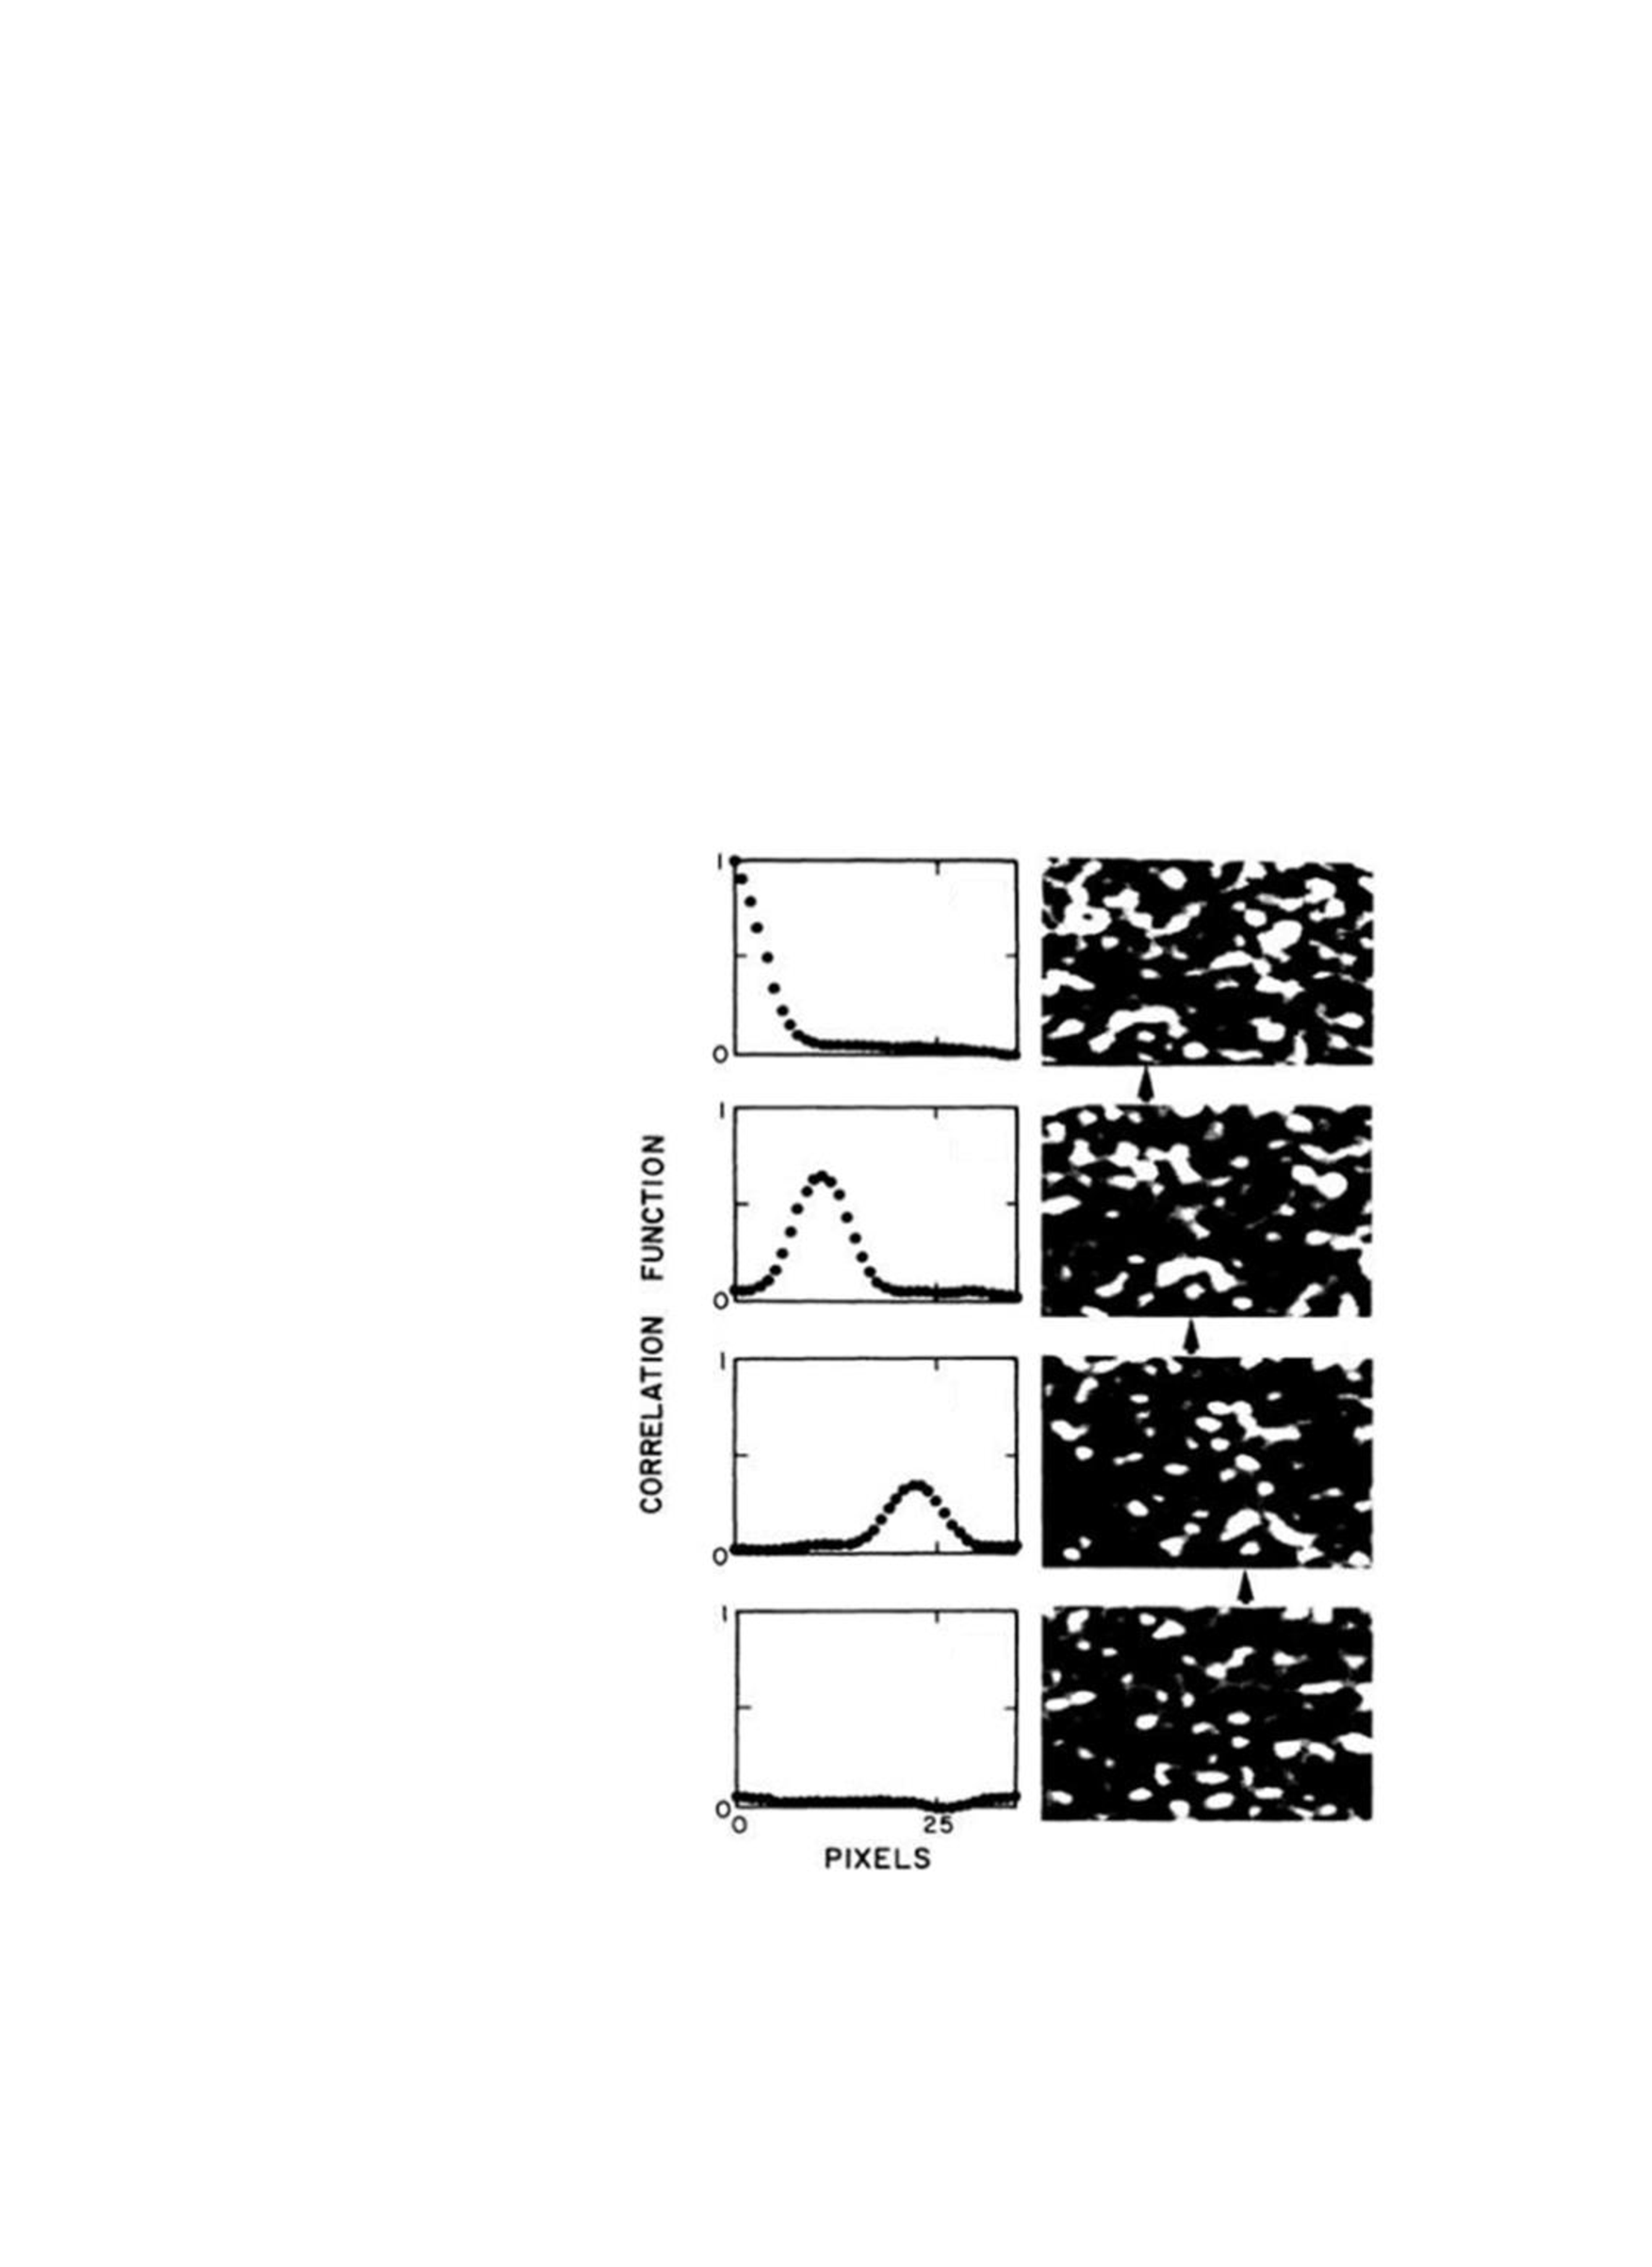
\includegraphics[scale=0.45]{C2.fig9}
	\caption{光学记忆效应实验结果}
	\label{fig2:9}
\end{figure}

随着对不同介质特性、传输矩阵和光学记忆效应的深入研究,光学记忆效应被分为三种类型:倾斜光学记忆效应,平移光学记忆效应和倾斜平移混合光学记忆效应。三种不同的光学记忆效应示意图如图\ref{fig2:21}所示,图\ref{fig2:21}(a)为倾斜光学记忆效应\cite{Freund1988};图\ref{fig2:21}(b)为平移光学记忆效应\cite{judkewitz_translation_2015};图\ref{fig2:21}(c)为倾斜平移混合光学记忆效应\cite{osnabrugge_generalized_2017}。
值得注意的是:平移光学记忆效应和倾斜平移混合光学记忆效应在透过厚散射介质聚焦或者成像有着更广泛的应用。

\begin{figure}[htp]
	\centering
	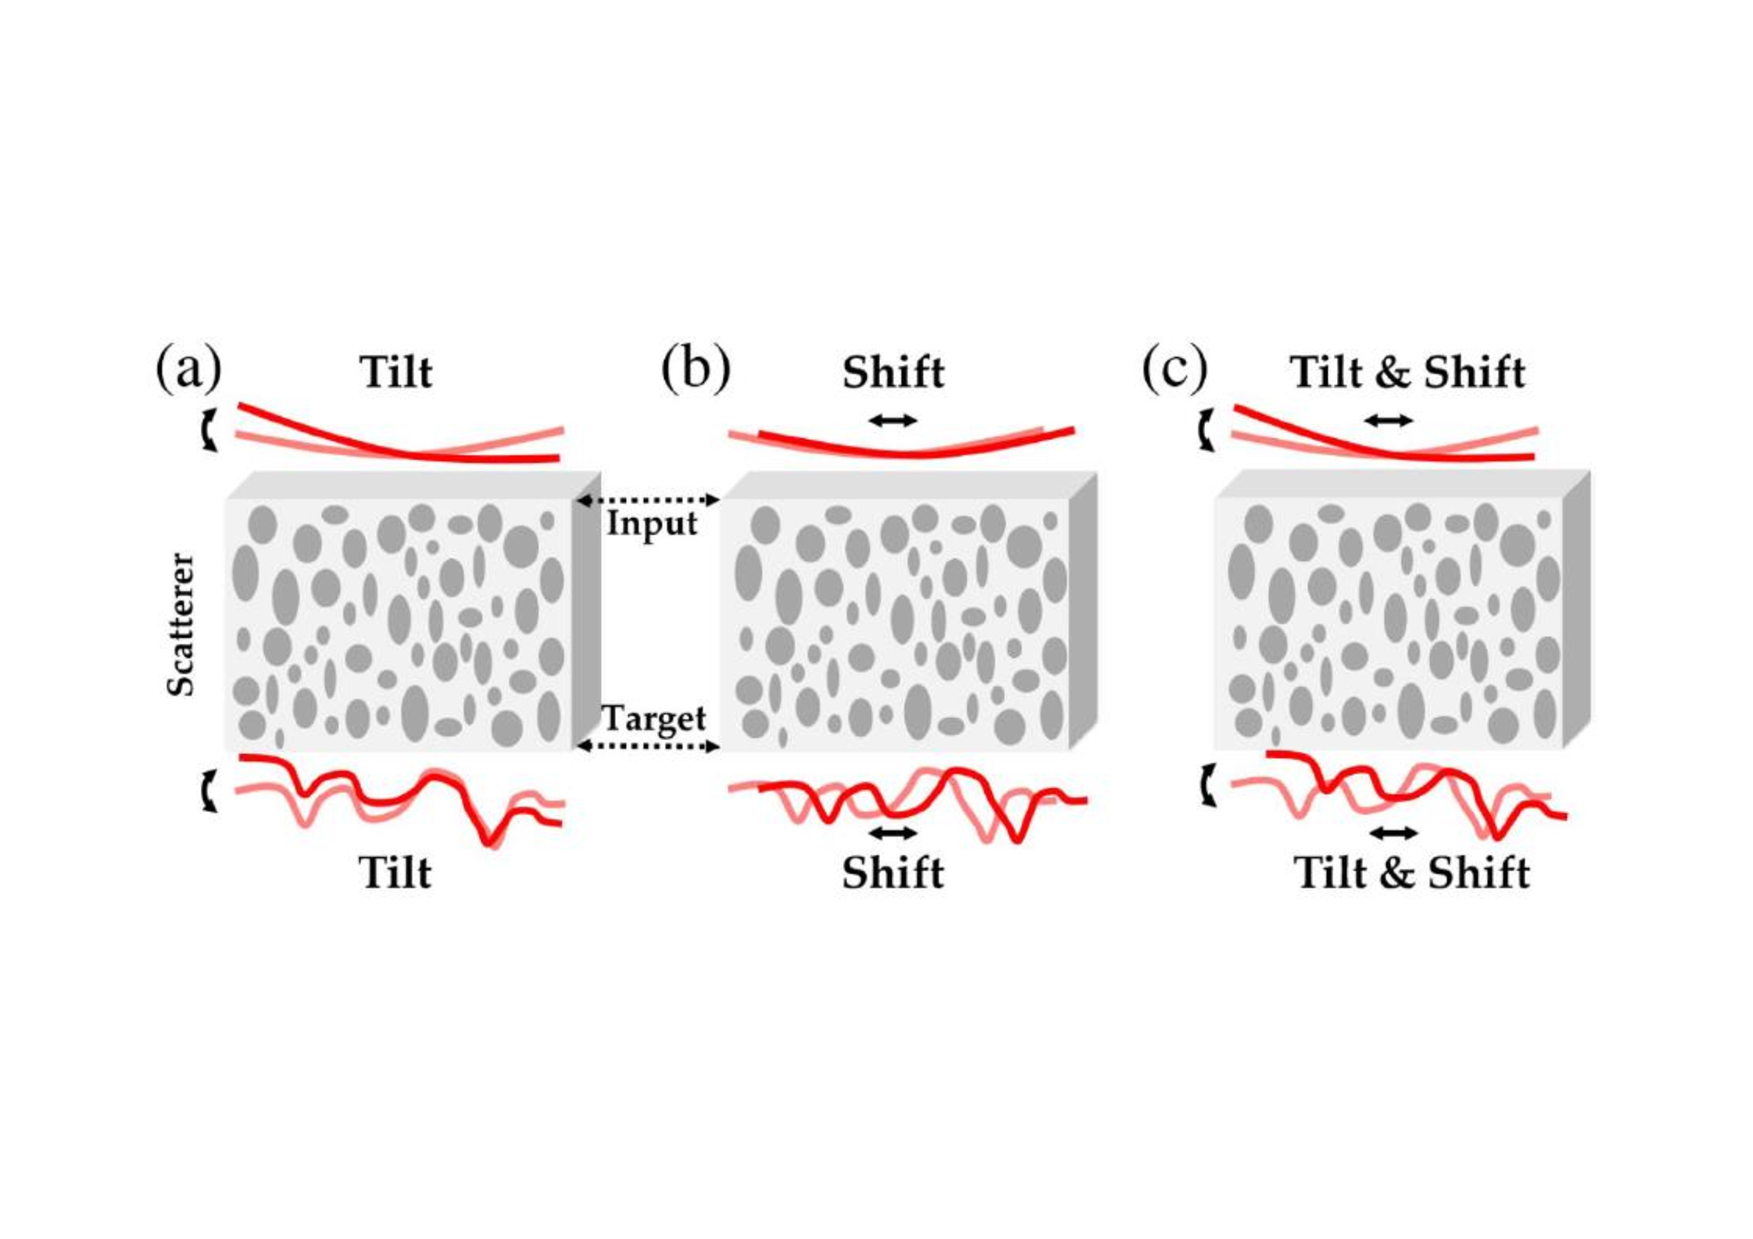
\includegraphics[scale=0.45]{C2.fig21}
	\caption{三种不同光学记忆效应类型}
	\label{fig2:21}
\end{figure}

\subsection{基于散斑相关的散射成像技术}

2012年,Bertolotti等人在Nature杂志上首次提出了利用散斑相关技术实现非侵入式的透过散射介质成像,实验系统如图\ref{fig2:10}所示。根据散射介质的记忆效应,激光器在空间中以不同角度$\theta$扫描时,相机接收到的散斑$I(\theta)$具有高度相关性,这一成像过程可以描述为

\begin{equation}
  I(\theta)= \int_{-\infty}^{\infty} O(r)S(r-\theta d) d^2 r = [O*S](\theta)
\label{eq:2.4}
\end{equation}
即散斑可以看成是原目标$O(r)$与上述成像系统点扩展函数$S(r)$卷积的结果,$r$表示空间位置,目标信息已经被“编码”至散斑中,$d$为散射介质与探测器之间距离。对散斑作自相关运算,并运用卷积定理可以得到

\begin{equation}
  \langle I\bigstar I \rangle = \langle O*S \rangle \bigstar \langle O*S \rangle = [O \bigstar O] * \langle S\bigstar S \rangle
\label{eq:2.5}
\end{equation}
式中:$\langle \rangle$为均值运算;$\bigstar$为相关运算;$*$为卷积运算。

\begin{figure}[htp]
	\centering
	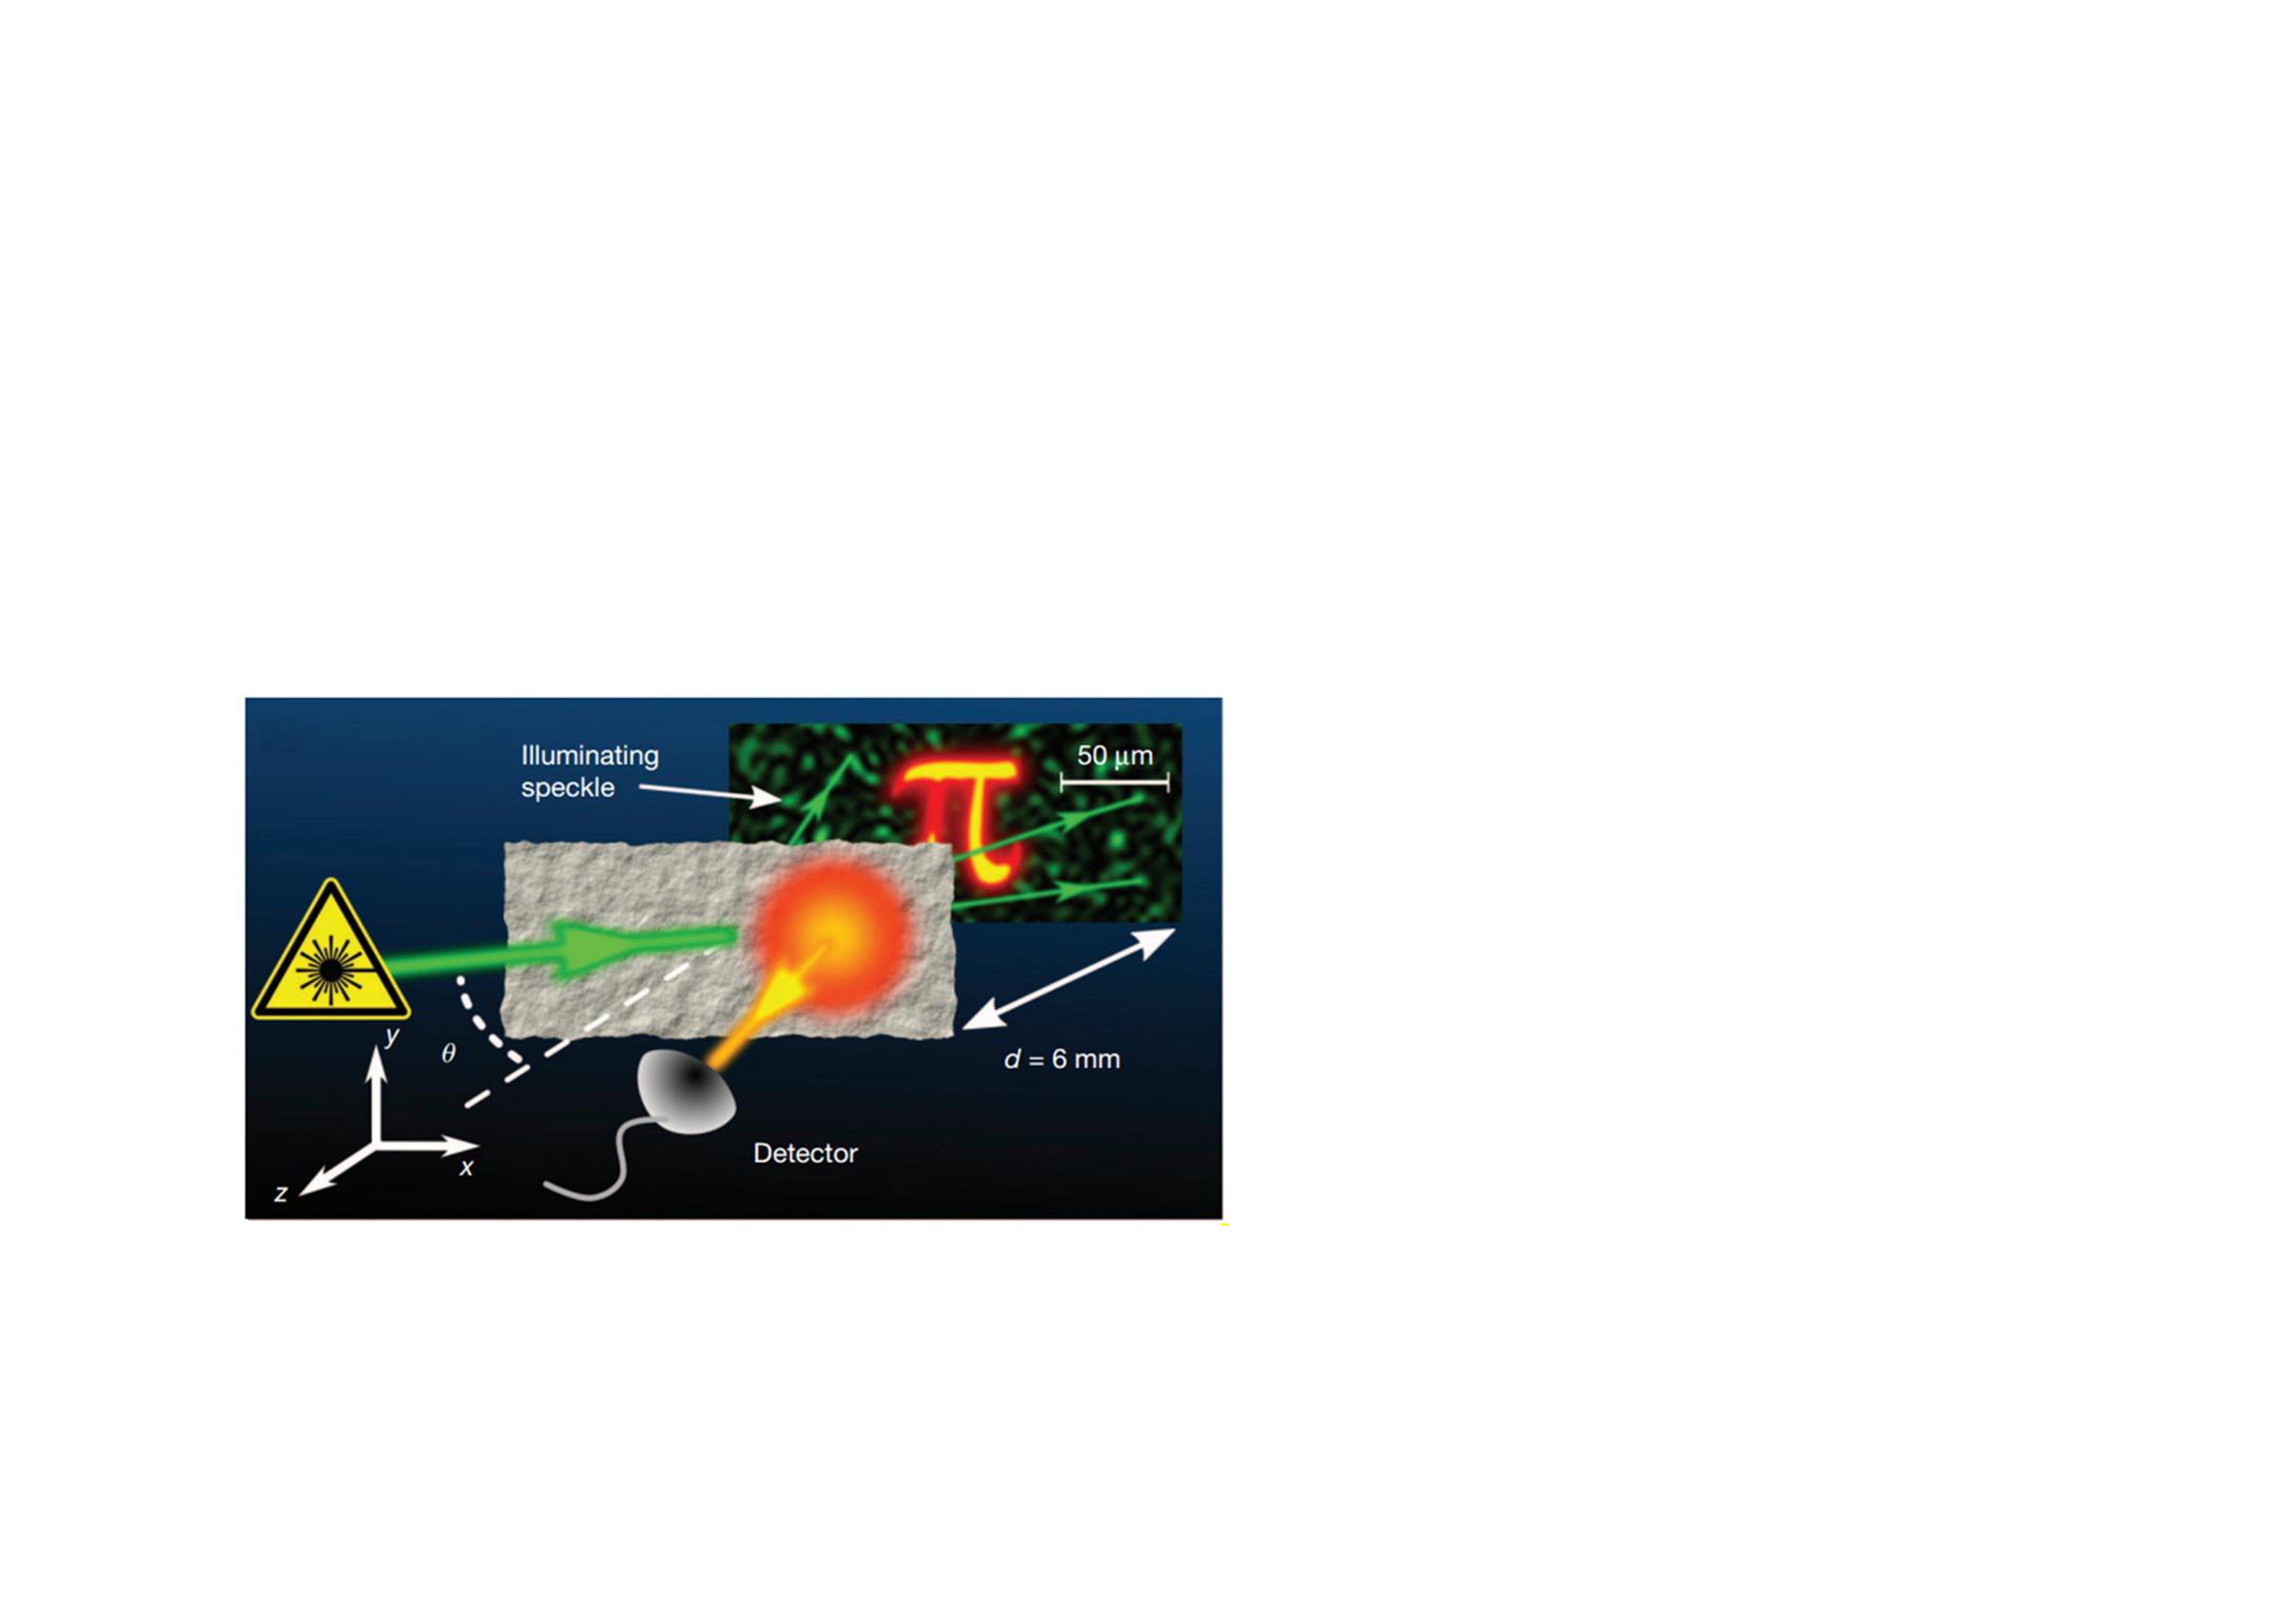
\includegraphics[scale=0.45]{C2.fig10}
	\caption{基于光学记忆效应的非侵入式成像方法示意图}
	\label{fig2:10}
\end{figure}

\begin{figure}[htp]
	\centering
	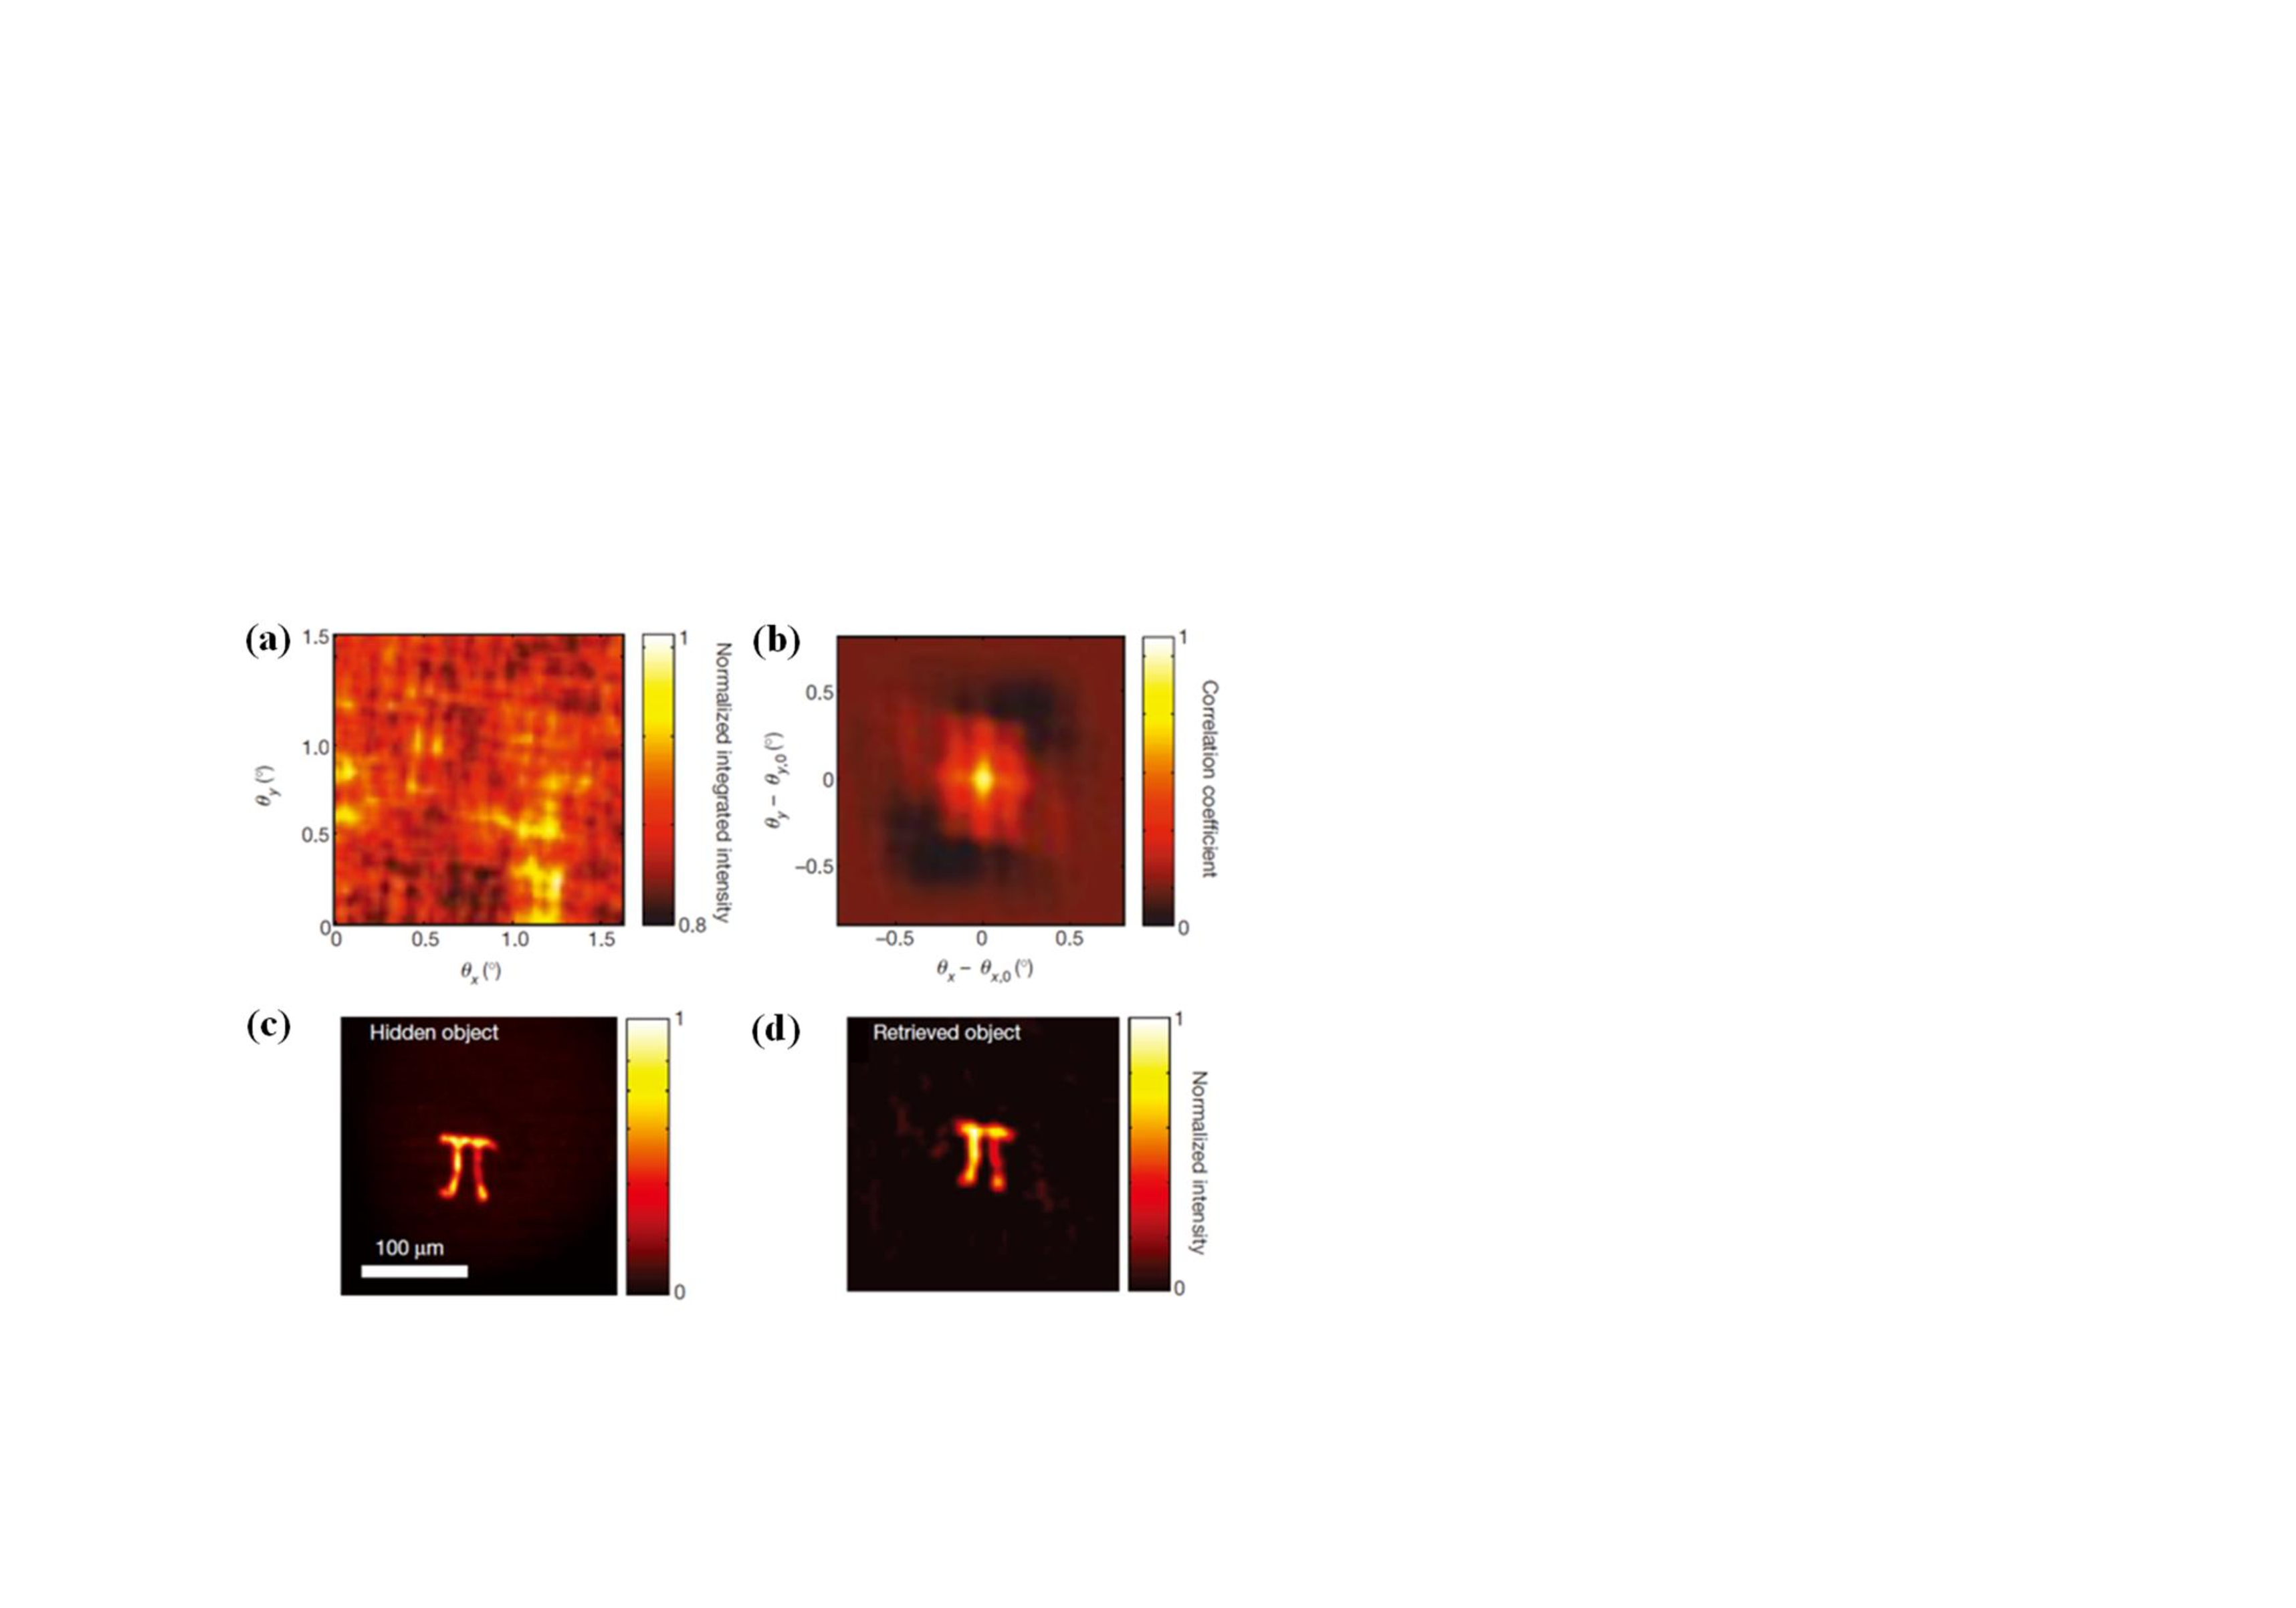
\includegraphics[scale=0.450]{C2.fig11}
	\caption{基于光学记忆效应的散射成像方法的实验结果}
	\label{fig2:11}
\end{figure}

依据介观物理理论,当介质的有效厚度远小于Anderson localization长度,并且散射足够充分时, 可以表示为类$\delta$函数,即目标的自相关信息可近似由散斑自相关得到。由Wiener-Khinchin定理可知,从目标的自相关信息中可以得到目标在频率域的振幅信息,再结合相位恢复算法采用迭代的方法就可以得到目标在频率域的相位信息,从而实现目标的重建,实验结果如图\ref{fig2:11}所示,图\ref{fig2:11}(a)为散斑;图\ref{fig2:11}(b)为散斑自相关结果;图\ref{fig2:11}(c)为原目标;图\ref{fig2:11}(d)为重建目标。该方法避免了波前整形及传输矩阵测量所带来的问题,极大地改善了已有方法的不足,但它仍需要在光学记忆效应范围内扫描,整个成像过程需要耗费几十分钟,依然无法满足实时成像的要求。


\begin{figure}[htp]
	\centering
	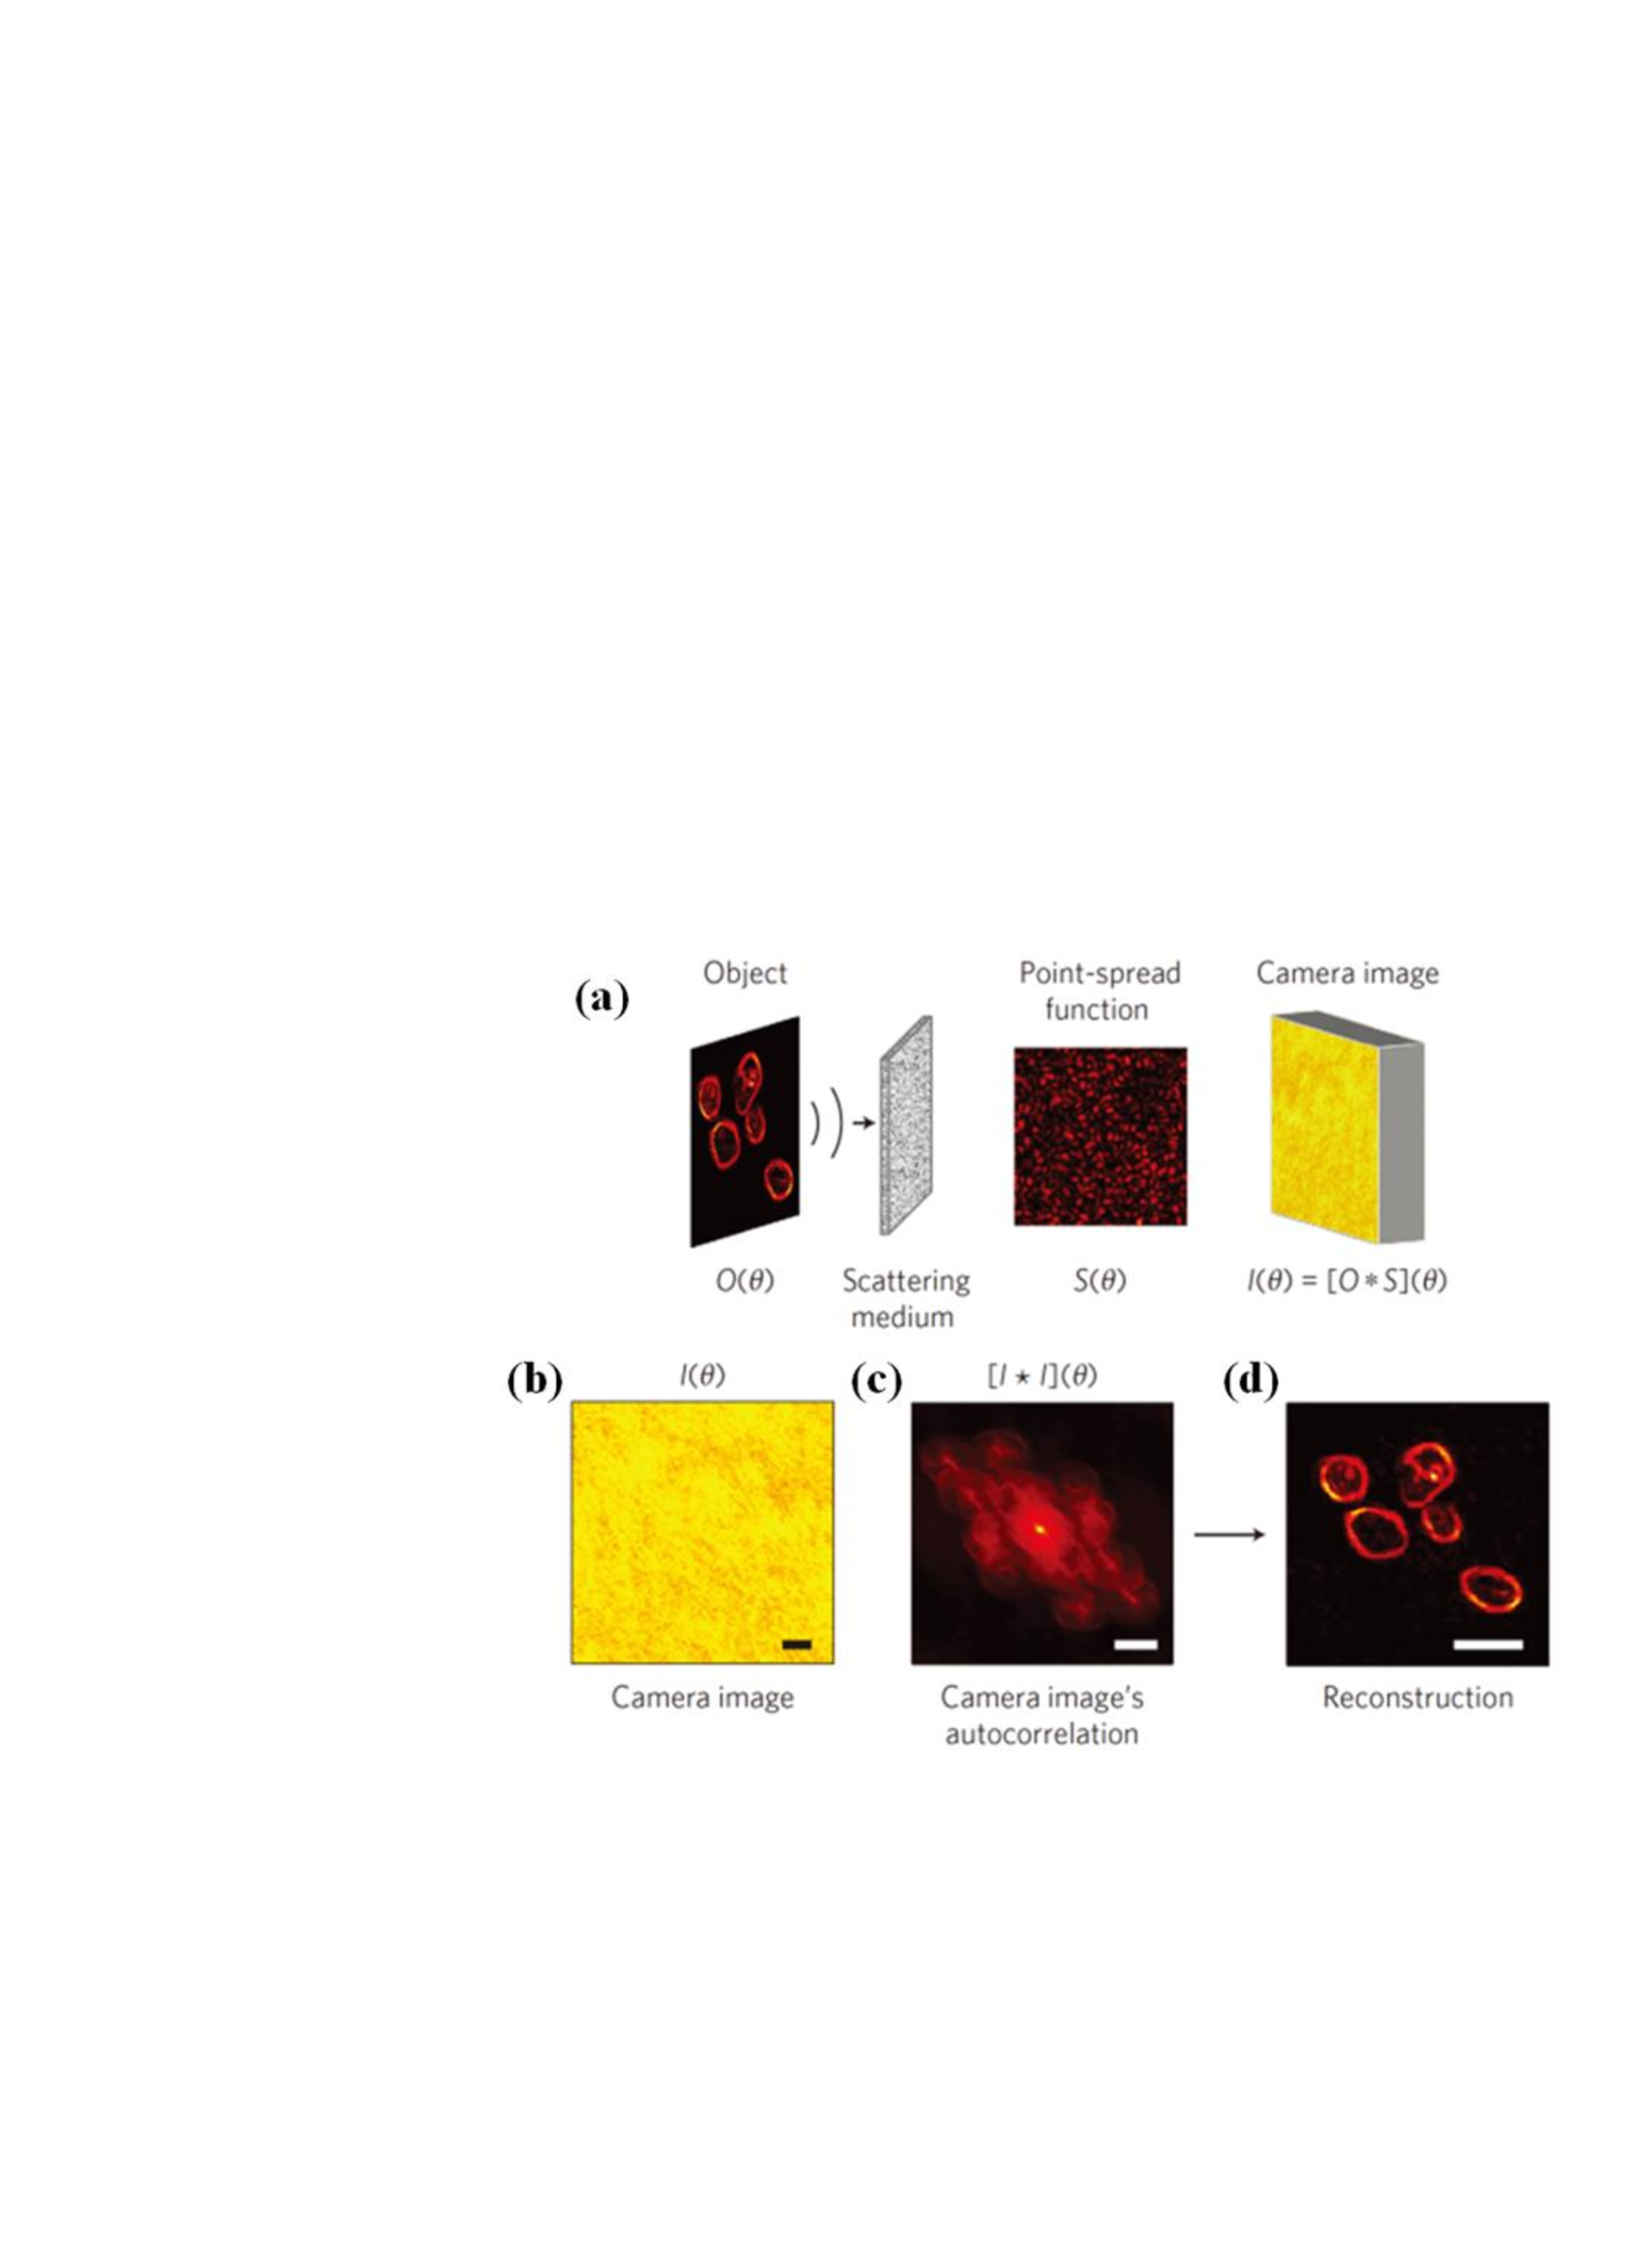
\includegraphics[scale=0.50]{C2.fig12}
	\caption{基于单帧散斑自相关成像的示意图}
	\label{fig2:12}
\end{figure}
\begin{figure}[htp]
	\centering
	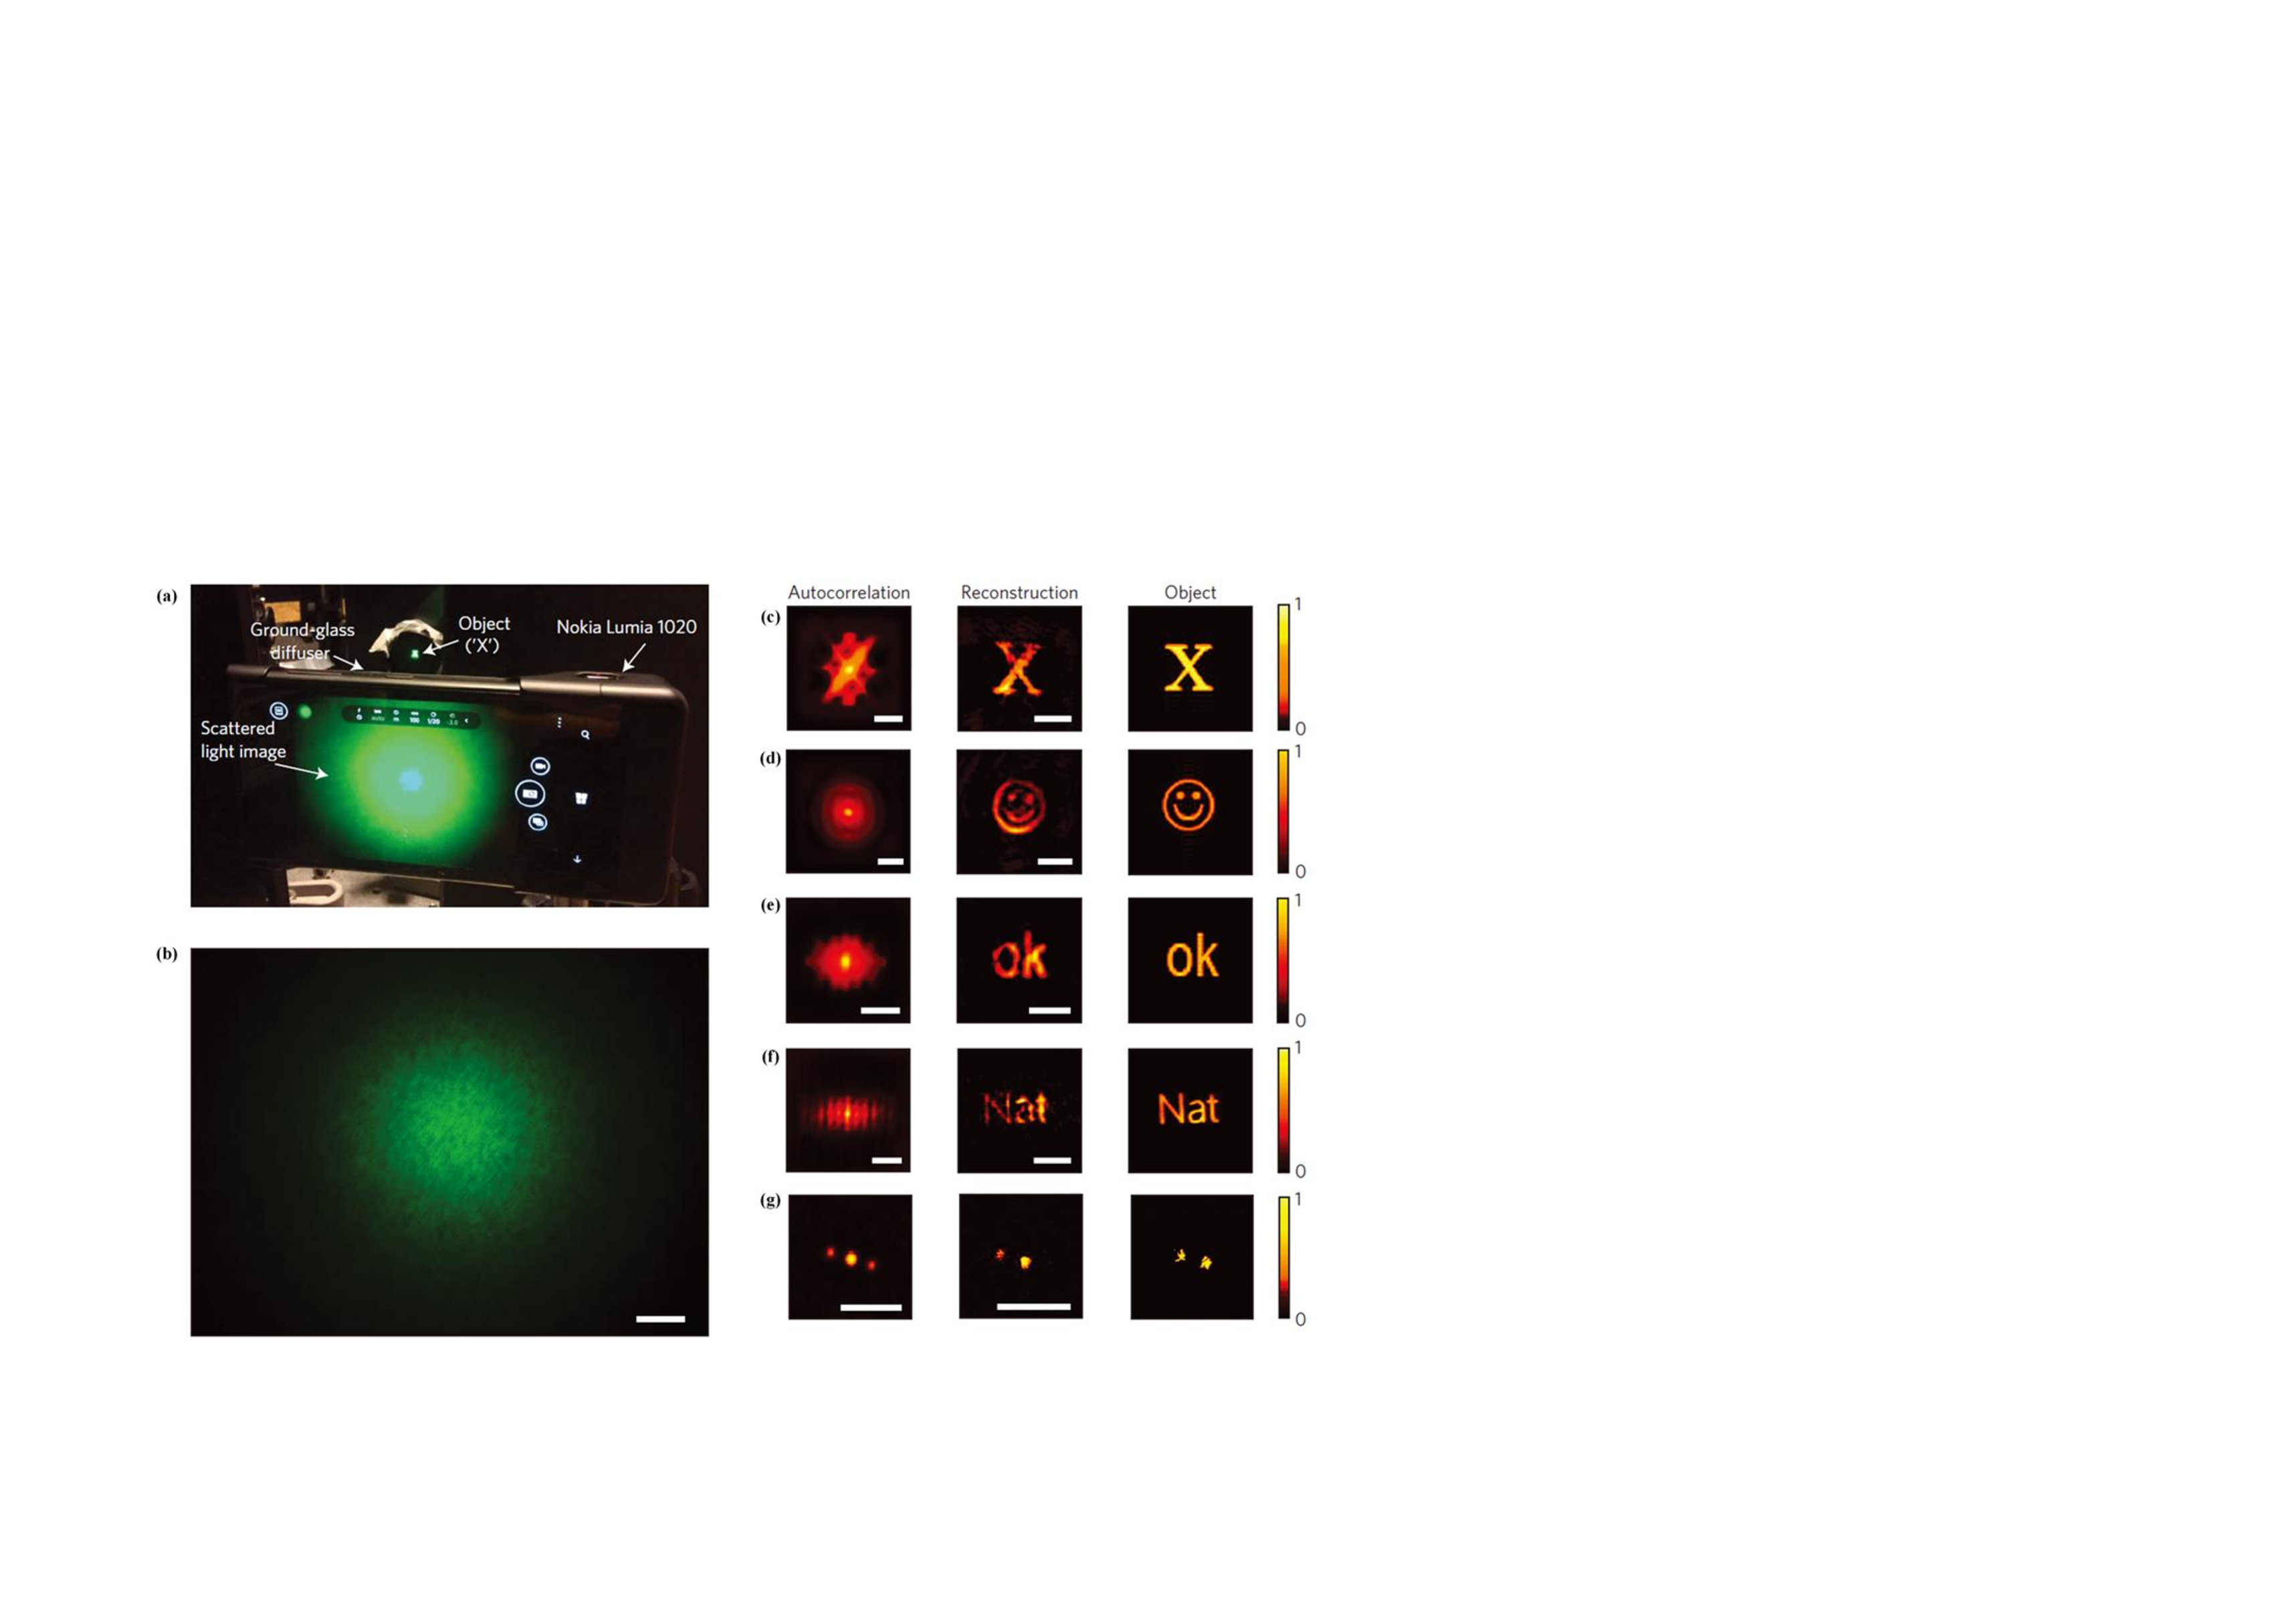
\includegraphics[scale=0.40]{C2.fig13}
	\caption{基于单帧散斑自相关成像的实验结果}
	\label{fig2:13}
\end{figure}
2014年,Katz等在Bertolotti研究的基础上提出了一种基于单帧散斑自相关的成像方法,成像模型和实验结果分别如图\ref{fig2:12}和图\ref{fig2:13}所示。图\ref{fig2:12}中,图\ref{fig2:12}(a)为成像模型示意图;图\ref{fig2:12}(b)为散斑图案;图\ref{fig2:12}(c)为散斑图案的自相关;图\ref{fig2:12}(c)为目标的重建结果。图\ref{fig2:13}中,图\ref{fig2:13}(a)为成像装置;图\ref{fig2:13}(b)为散斑;图\ref{fig2:13}(c)~(g)第一列为散斑自相关,第二列为重建目标,第三列为原目标。该方法不仅完全避免了原有成像方法需要扫描的缺陷,而且避免了成像系统的像差带来的影响,节省了成像时间,成为散射成像技术的又一次突破。然而,该方法依然受限于光学记忆效应,并且实现非侵入式的条件比较苛刻,距离实际应用依然存在很多障碍。同时,该方法的成像效果会受到相位恢复算法的影响,成像存在不确定性。如:Fienup型相位恢复算法的缺点在于,初始迭代相位的随机性导致最终的重建目标在方向、空间位置上具有随机性,进而导致了重建结果的不确定性。

\begin{figure}[htp]
	\centering
	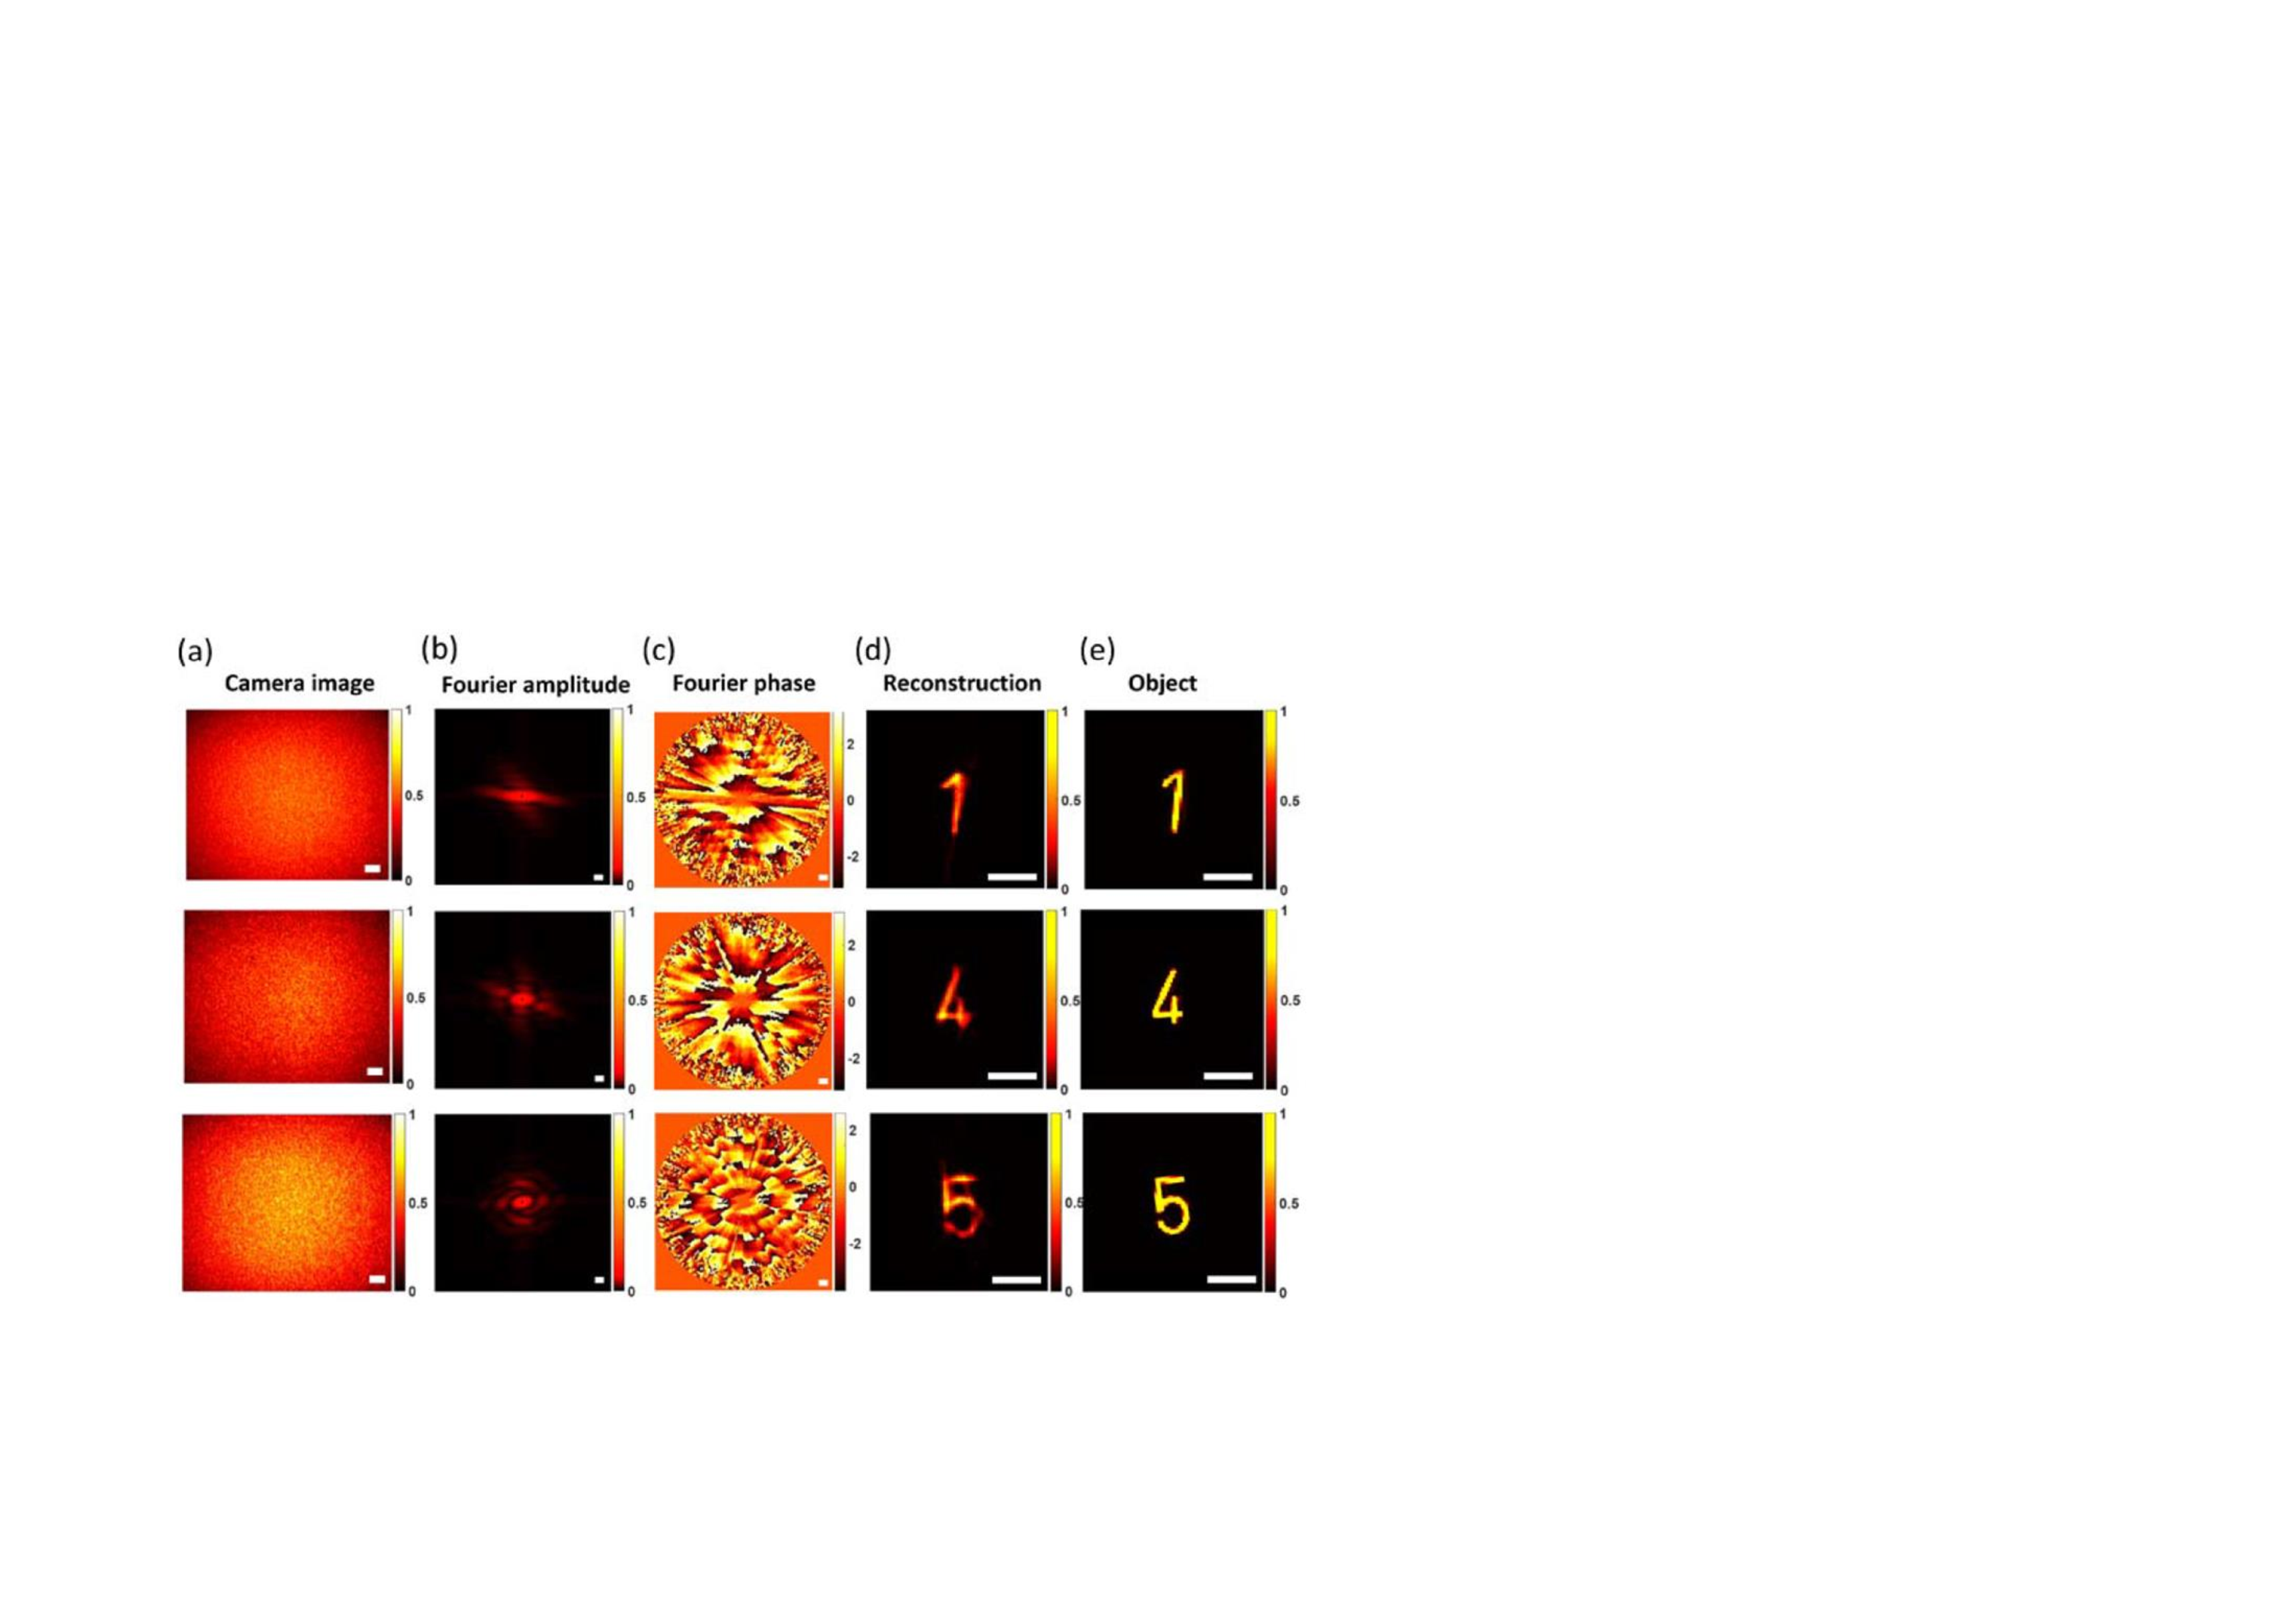
\includegraphics[scale=0.45]{C2.fig14}
	\caption{采用双谱分析得到的重建结果}
	\label{fig2:14}
\end{figure}

针对Fienup型相位恢复算法的缺点,Wu等将天文观测中的三阶相关相位恢复技术(又称双谱技术)引入到散射成像的相位恢复过程中,用以解决由相位恢复算法所导致的重建结果不确定的问题。采用双谱分析得到的重建结果如图\ref{fig2:14}所示,图\ref{fig2:14}(a)为散斑;图\ref{fig2:14}(b)为傅里叶振幅;图\ref{fig2:14}(c)为傅里叶相位;图\ref{fig2:14}(d)为重建目标;图\ref{fig2:14}(e)为原目标。三阶相关相位恢复技术与Fienup型相位恢复算法的散斑相关成像相比具有以下优势:1)能够精确地恢复出目标频率域的相位信息;2)不需要大量的迭代与重复估计;3) 具有更好的抗噪性;4)保留了目标的方向信息。

除了上文所提到的静态散射介质,透过动态散射介质成像是透过散射介质成像领域不可或缺的一部分。2016年,美国马里兰大学的Scarcelli课题组提出了一种基于浴帘效应的散射成像方法。该方法通过对多帧散斑作逆傅里叶变换并叠加取平均值,近似求得了原目标场的自相关,然后结合相位恢复算法得到了目标的频率域相位,进而恢复出了目标信息,如图\ref{fig2:15}所示。在图\ref{fig2:15}中,图\ref{fig2:15}(a)为原目标;图\ref{fig2:15}(b)为薄散射体远离目标;图\ref{fig2:15}(c)为薄散射体紧贴目标;图\ref{fig2:15}(d)为基于浴帘效应的散射成像系统原理图;图\ref{fig2:15}(e)为目标重建过程。相比前述几种成像方法,基于浴帘效应的成像方法的主要不同之处在于:1)利用了散射介质的近场相关性;2)可适用于透过动态散射介质成像;3)照明光源为相干光。然而,其局限性也很明显,如需要记录多帧散斑,限制了成像速度。

\begin{figure}[htp]
	\centering
	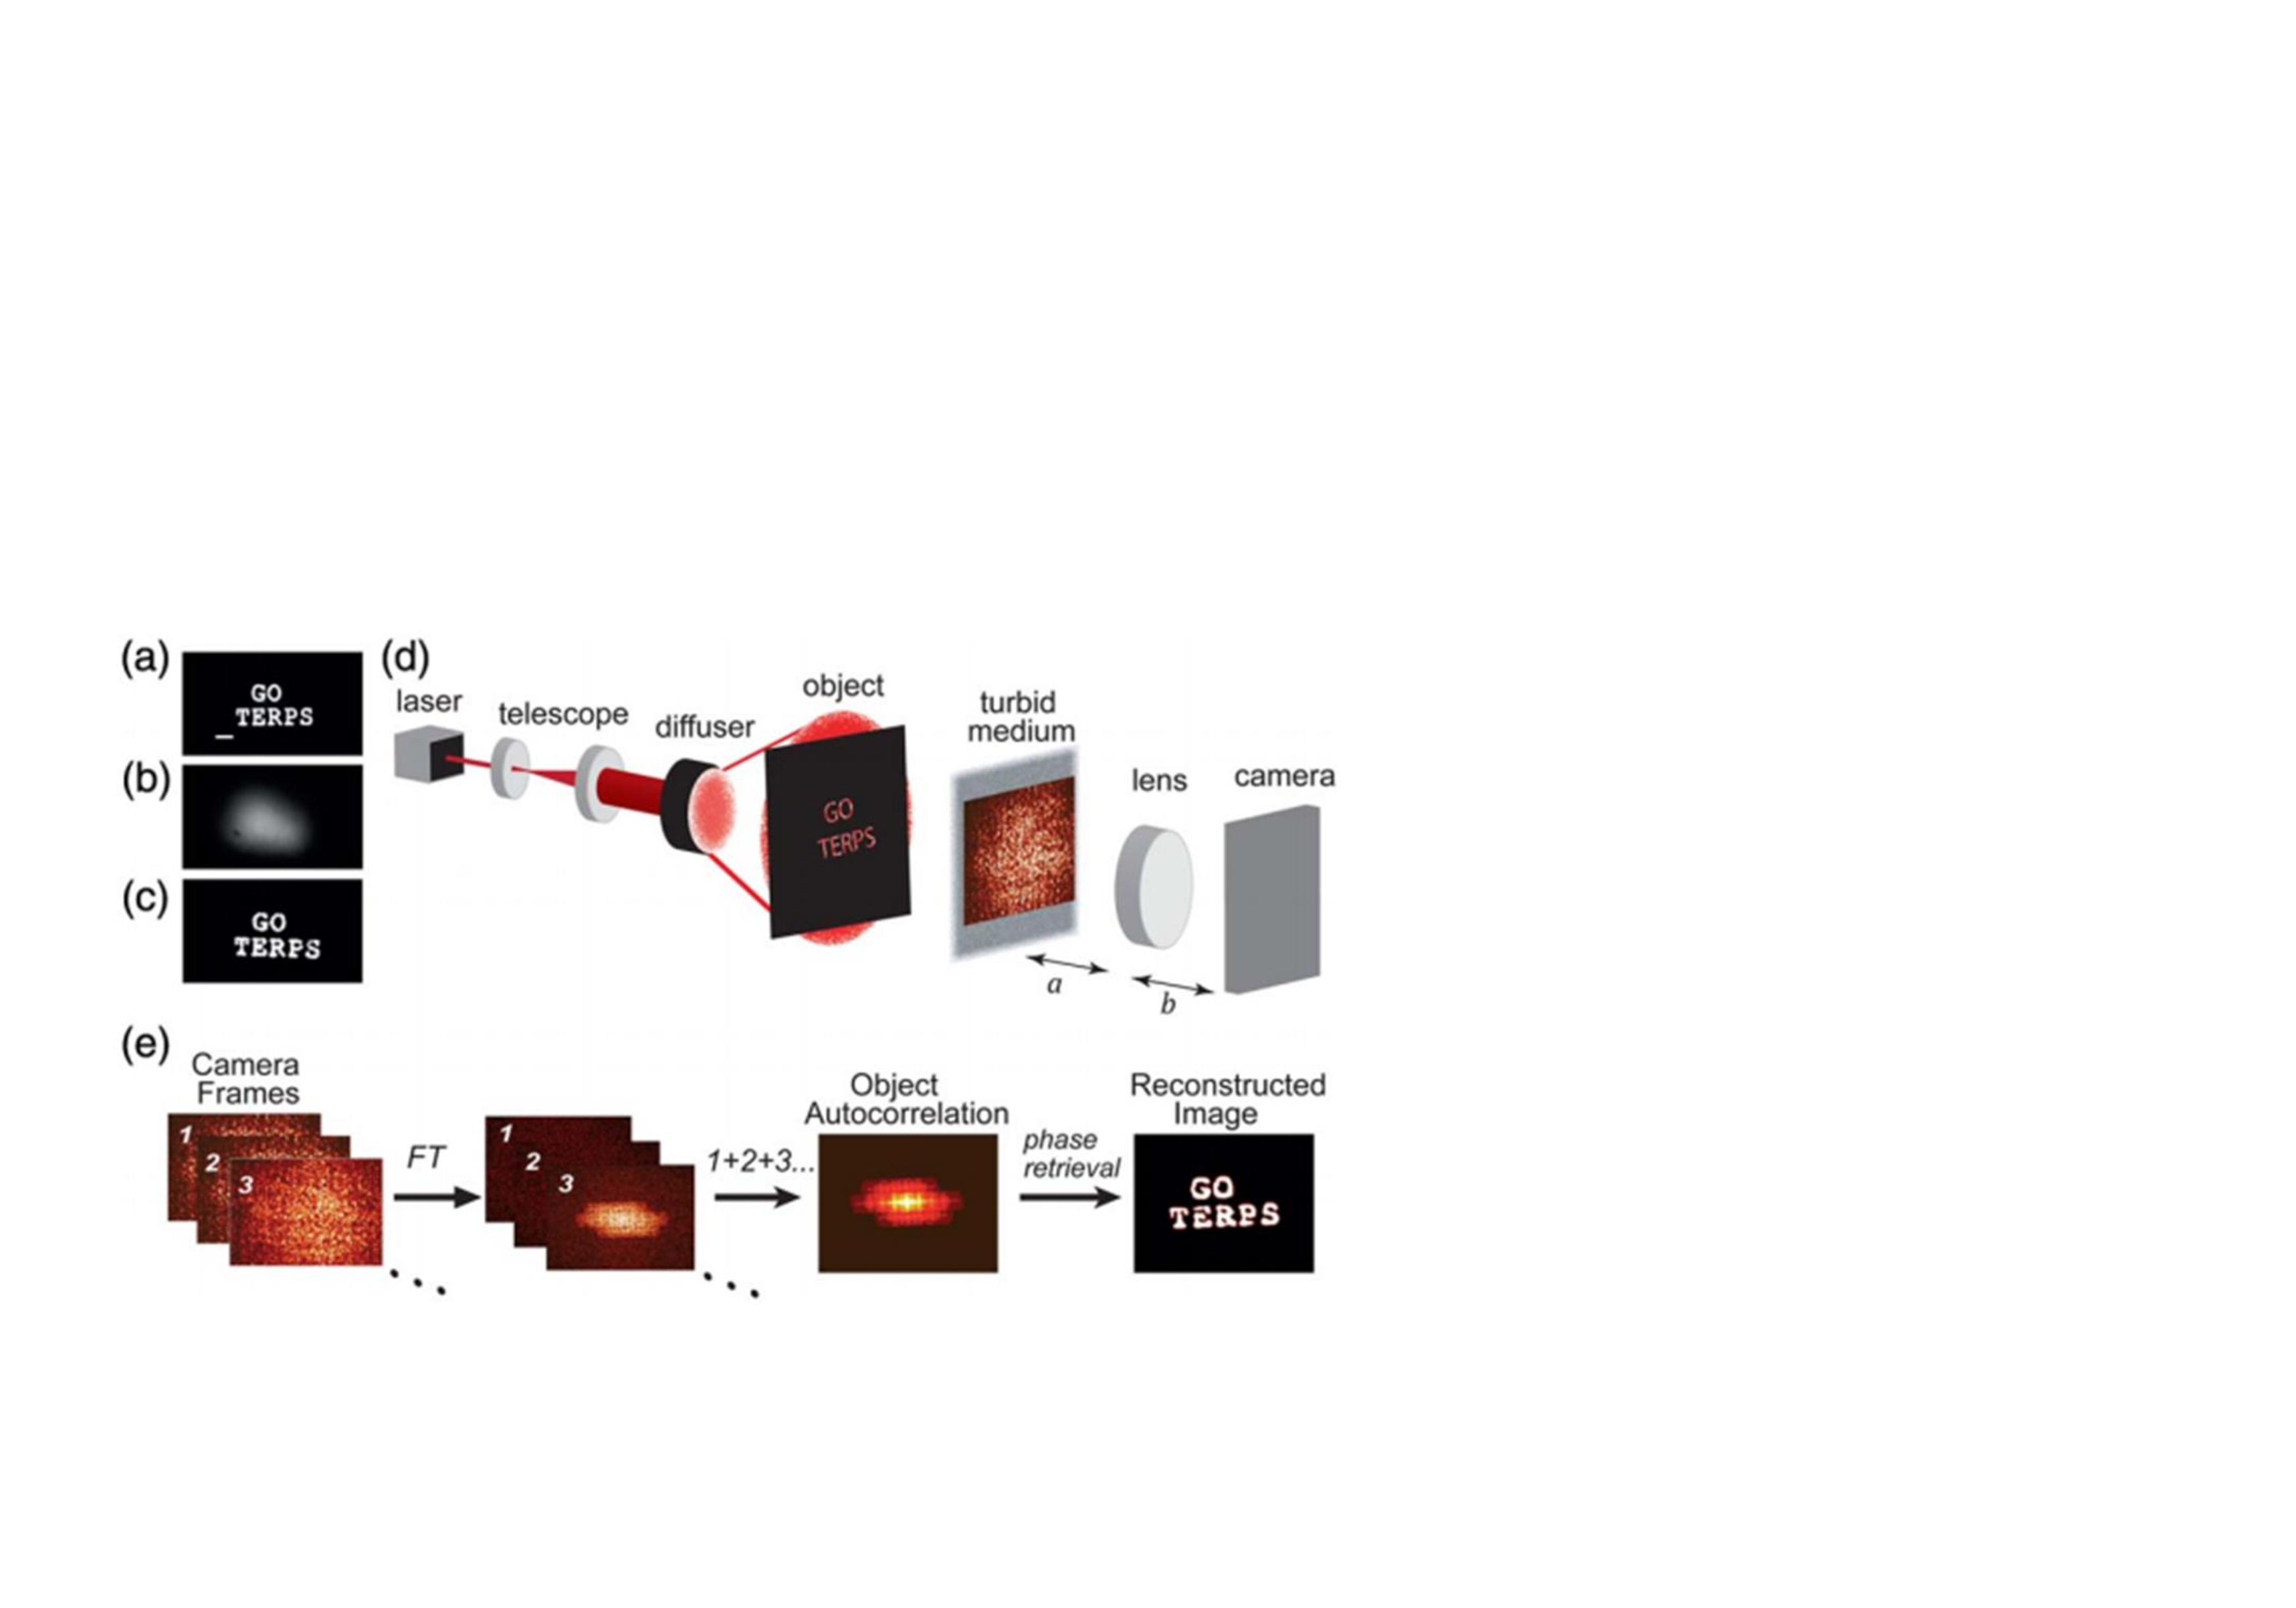
\includegraphics[scale=0.35]{C2.fig15}
	\caption{基于浴帘效应的散射成像结果}
	\label{fig2:15}
\end{figure}

基于散斑相关的散射成像方法具有系统简单且能够实现非侵入式成像的特点,但其缺点也很明显,如:成像的视场受记忆效应范围的限制,与平均传输自由程成反比。鉴于此,许多扩展光学记忆效应的方法和技术应运而生,如:利用参考目标或先验知识实现超记忆效应范围成像的技术,通过光场估计或散斑估计的方法实现透过散射介质成像的景深扩展。除了以上所描述的基于散斑相关的透过散射介质成像技术外,将散斑相关成像技术与光谱编码技术、压缩感知技术、双目视觉技术等相结合,也可实现透过散射介质的彩色成像、光谱成像和三维成像等。
\subsection{利用光学记忆效应点扫描成像技术}

光学记忆效应是无序介质的固有特性,可以用任何入射波前观察到。特别是,当入射波前在透射中形成一个明亮的焦点时,它也可以用来成像。如果介质拥有光学记忆效应,则意味着这个焦点可以被平移。这种点扫描成像方法对于透过散射介质成像特别有趣,因为使用单个焦点和光栅扫描它(基于“倾斜”记忆效应),可以恢复隐藏目标的图像。这种利用光学记忆效应实现点扫描成像首次被Vellekoop等人验证\cite{vellekoop_scattered_2010},如图\ref{fig2:22}所示。在图\ref{fig2:22}中,图\ref{fig2:22}(a)为平面波透过波散射介质形成散斑示意图;图\ref{fig2:22}(b)为基于波前整形技术聚焦示意图;图\ref{fig2:22}(c)为聚焦点扫描示意图;图\ref{fig2:22}(d)为实验系统;图\ref{fig2:22}(e)为目标图像;图\ref{fig2:22}(f)为扫描成像结果;图\ref{fig2:22}(f)为相机所接收到散斑图案。

\begin{figure}[htp]
	\centering
	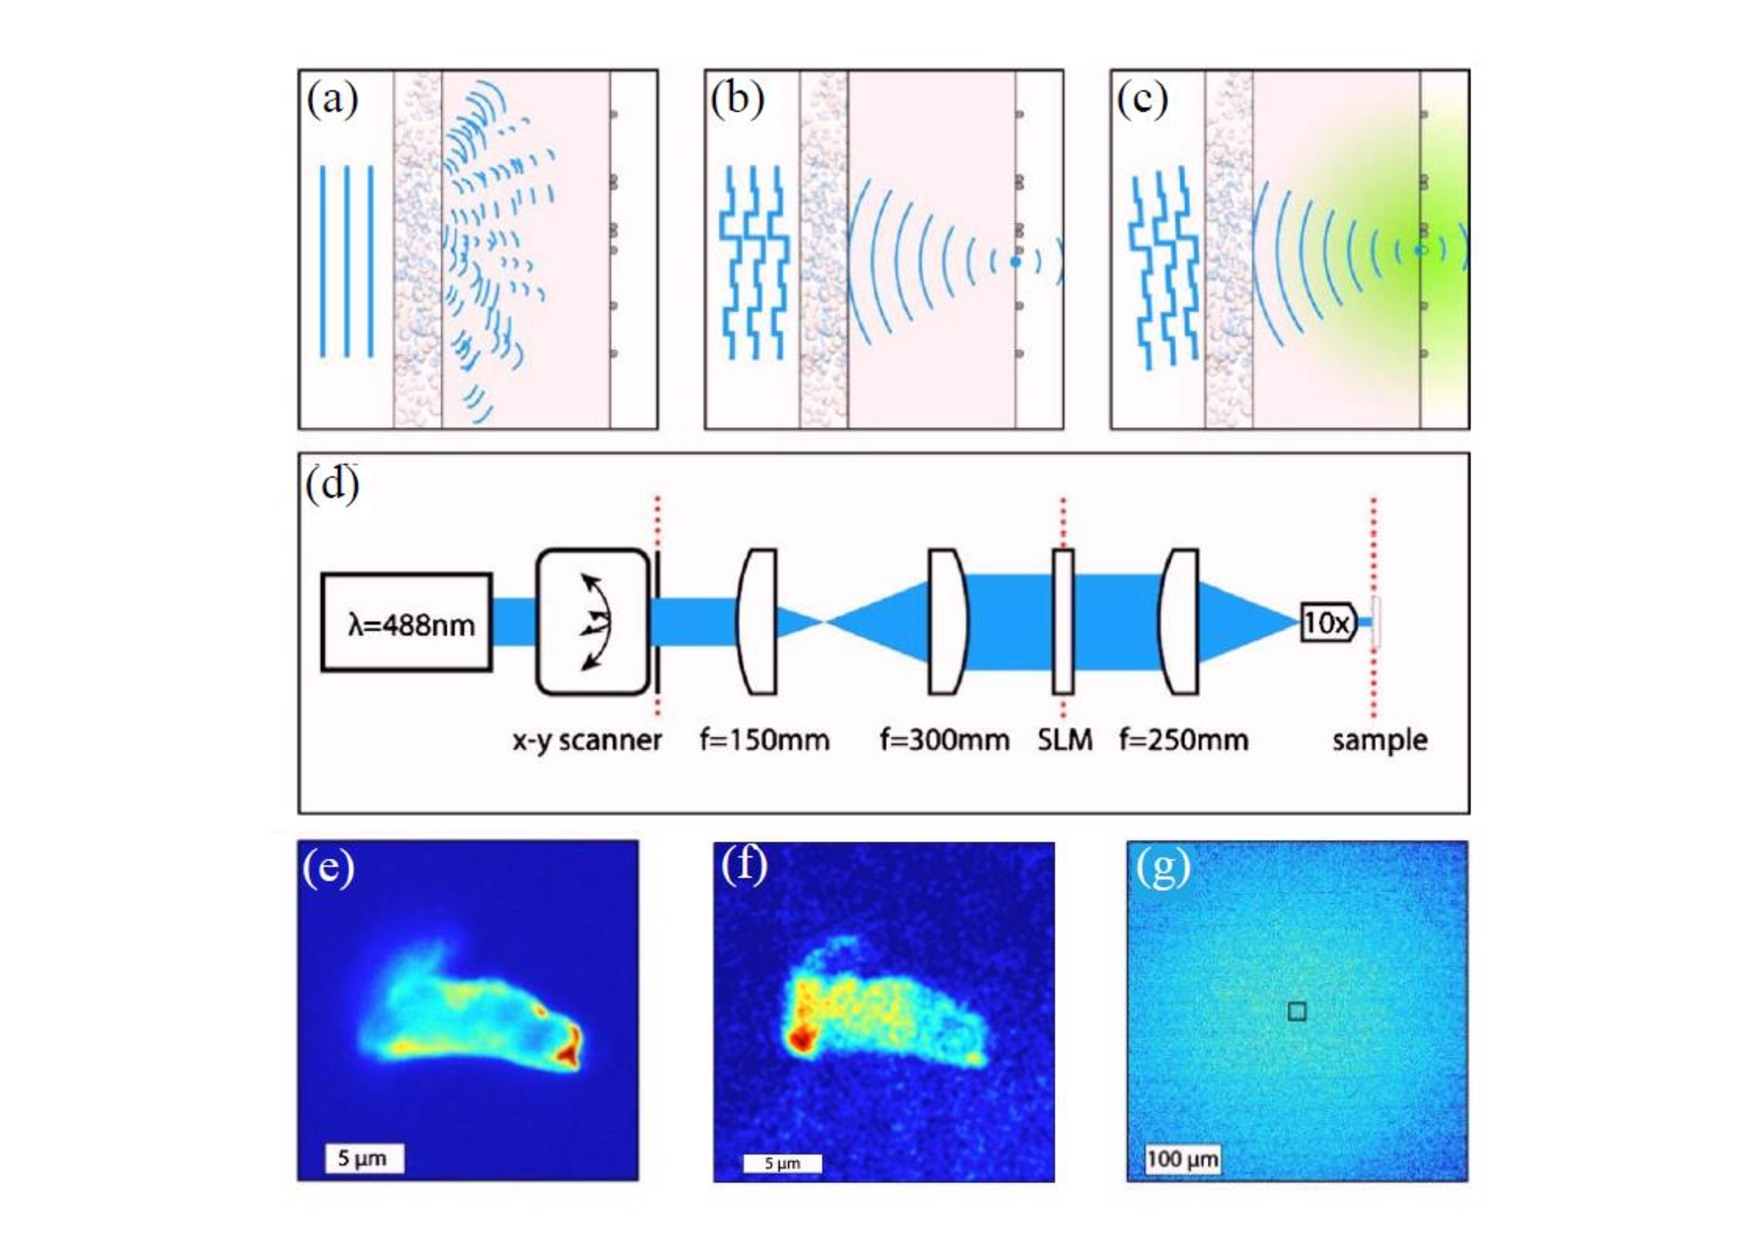
\includegraphics[scale=0.45]{C2.fig22}
	\caption{基于光学记忆效应的点扫描成像结果}
	\label{fig2:22}
\end{figure}

\section{基于点扩展函数工程的透过散射介质成像技术}

根据光学效应范围,透过散射介质成像系统的数学模型如式(\ref{eq:2.4})所示,分析其数学模型不难发现,在传统成像方面已成熟应用的去卷积技术有望实现透过散射介质成像。2016年,Edrei等在测量散射系统点扩展函数的基础上,采用Lucy-Richardson去卷积迭代非线性复原方法,实现了透过散射介质成像,结果如图\ref{fig2:16}所示。图\ref{fig2:16}中,图\ref{fig2:16}(a)为实验系统示意图;图\ref{fig2:16}(b)为原目标;图\ref{fig2:16}(c)为散斑图案;图\ref{fig2:16}(d)为系统点扩展函数;图\ref{fig2:16}(e)为重建结果。Edrei等开创了利用点扩展函数实现透过散射介质成像的新局面,其核心在于系统点扩展函数的获取。点扩展函数工程的成像效果依赖于所获取的系统的点扩展函数的准确性,在成像过程中要保证散射介质的稳定性。基于点扩展函数工程的透过散射介质成像技术仅适用于静态散射介质成像。

\begin{figure}[htp]
	\centering
	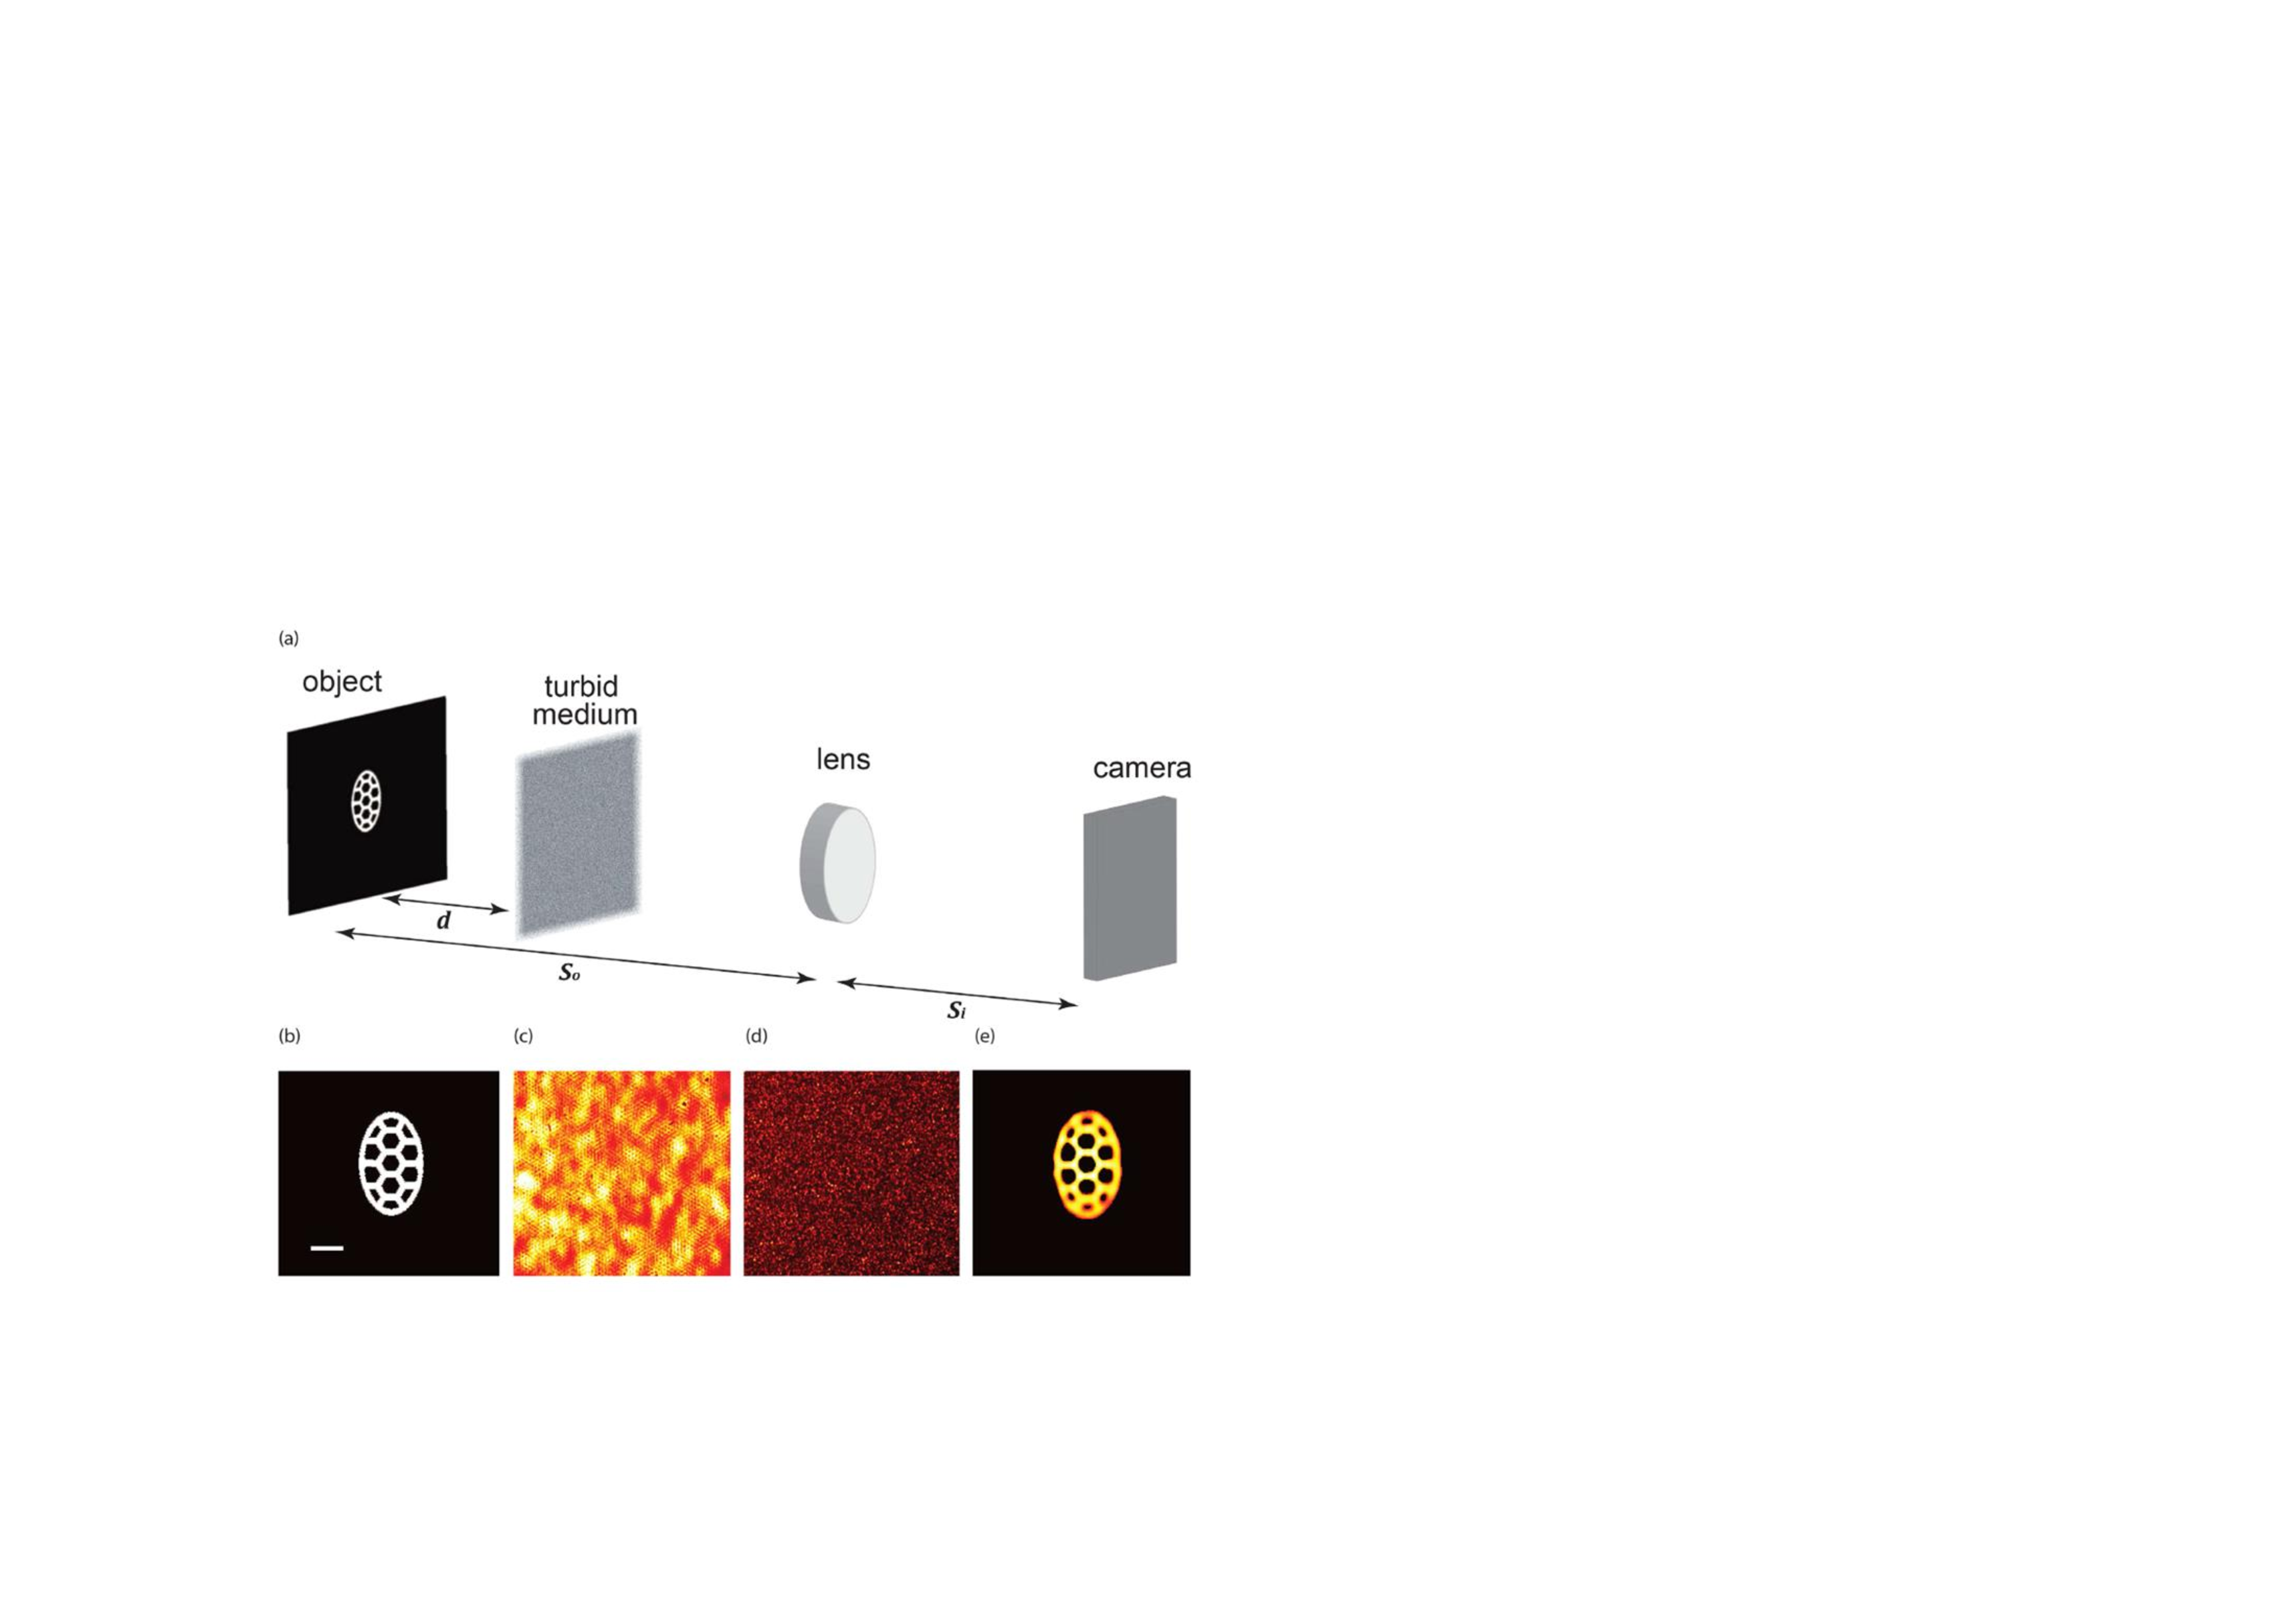
\includegraphics[scale=0.45]{C2.fig16}
	\caption{基于去卷积的散射成像结果}
	\label{fig2:16}
\end{figure}

2017年,西安电子科技大学的邵晓鹏课题组借鉴天文成像所应用的相位多样性技术,通过获取多帧散斑,估算得到了散射光学系统的点扩展函数,进而通过去卷积技术实现了透过散射介质成像。基于相位多样性的散斑成像原理、散斑重建及系统点扩展函数估计结果如图\ref{fig2:17}、\ref{fig2:18}所示,通过采集N帧多样性散斑,利用不同像平面位置处系统孔径函数中相位分布之间的关系,结合相位多样性重建方法,对系统的点扩展函数进行联合估计,进而通过去卷积方式实现了目标重构。与其他方法相比,该方法仅需多帧散斑进行联合估计,无须测量系统的点扩展函数便可实现透过散射介质成像。图\ref{fig2:18}中,图\ref{fig2:18}(a)为原目标;图\ref{fig2:18}(b)为多样性散斑;图\ref{fig2:18}(c)第一列为估计的随机相位,第二列为估计的局部点扩展函数,第三列为重建目标。

\begin{figure}[htp]
	\centering
	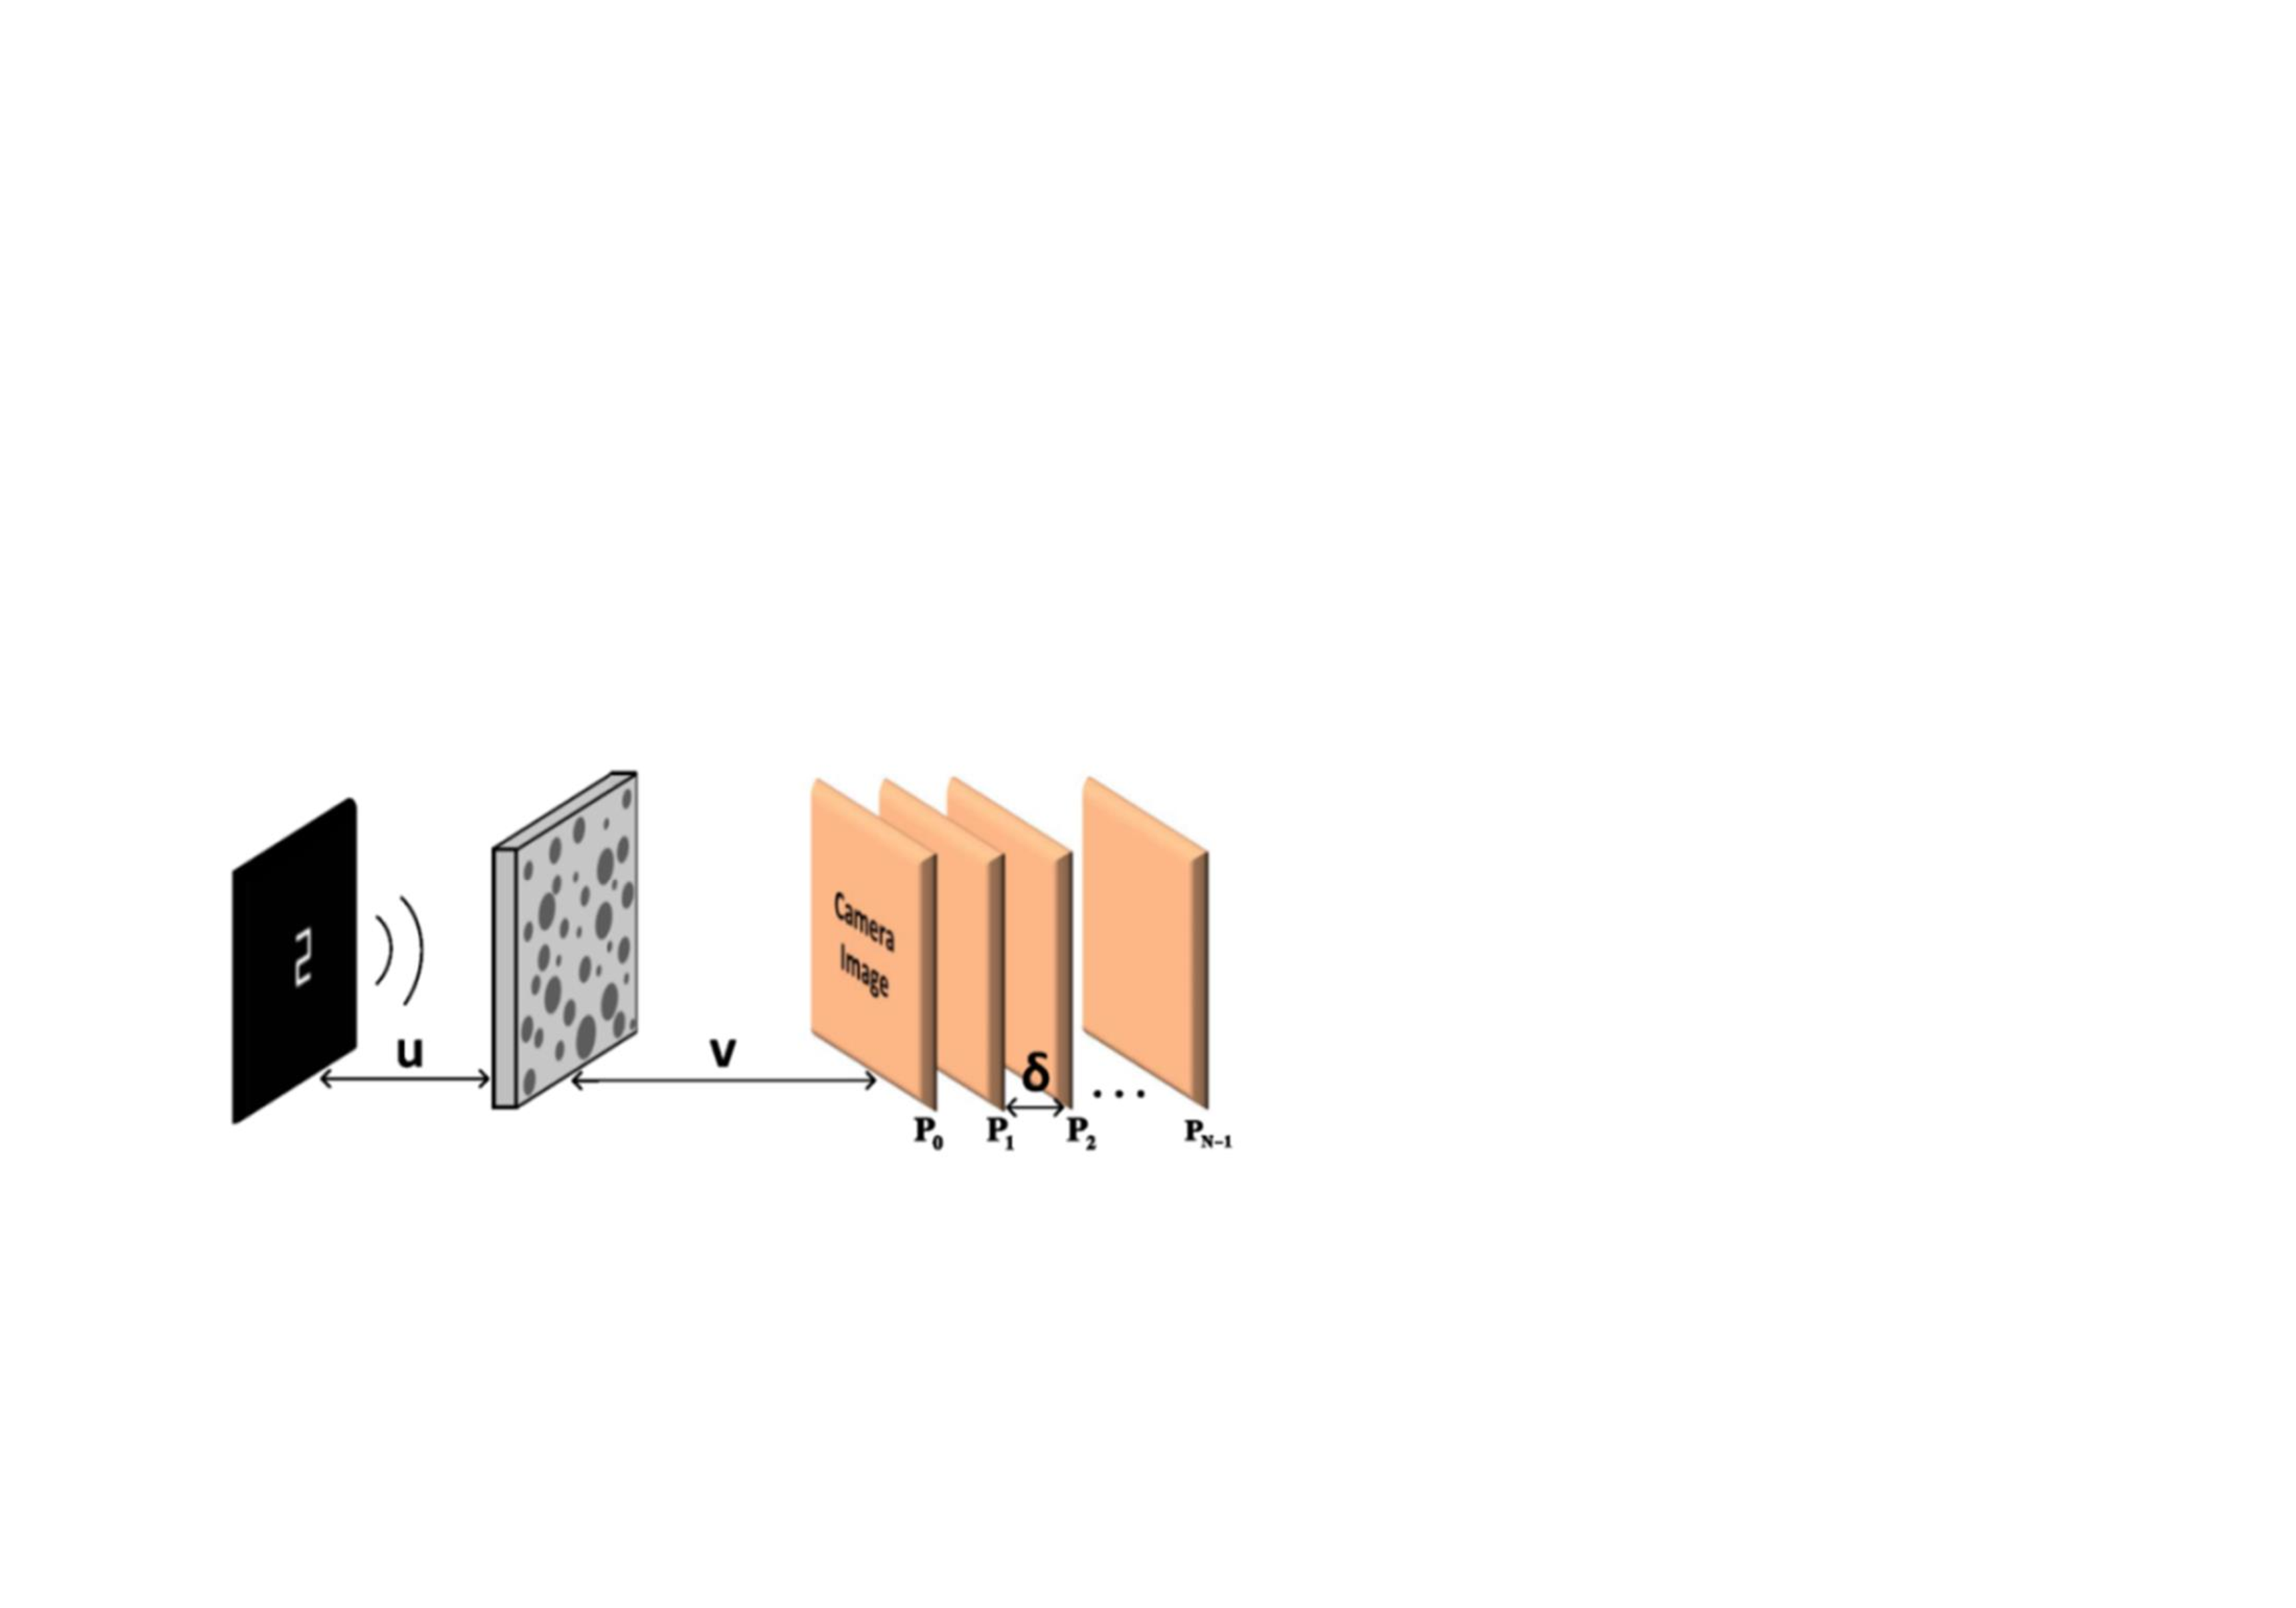
\includegraphics[scale=0.35]{C2.fig17}
	\caption{基于相位多样性的散斑成像原理示意图}
	\label{fig2:17}
\end{figure}

除了上文提到的利用去卷积或估计系统点扩展函数实现透过散射介质成像外,利用散射介质点扩展函数的光谱维和空域正交性,在光谱维或空域多次测量散射介质的点扩展函数,将解卷积得到的物体像进行数据重构,也可以实现透过散射介质的光谱成像和三维成像。例如:2017年,Sahoo等分别测量获得了散射系统在不同波长下的点扩展函数,利用散射介质的光谱退相关特性,将去卷积过程作为光谱滤波的手段,实现了单帧透过散射介质多光谱成像;2018年,Antipa等利用空域中点扩展函数的正交特性,分别测量了物空间不同点源目标所产生的点扩展函数,通过3D-TV去卷积方式,实现了单帧透过散射介质的三维成像,重构过程具有稳定性高、抗噪性能较强的特点。

\begin{figure}[htp]
	\centering
	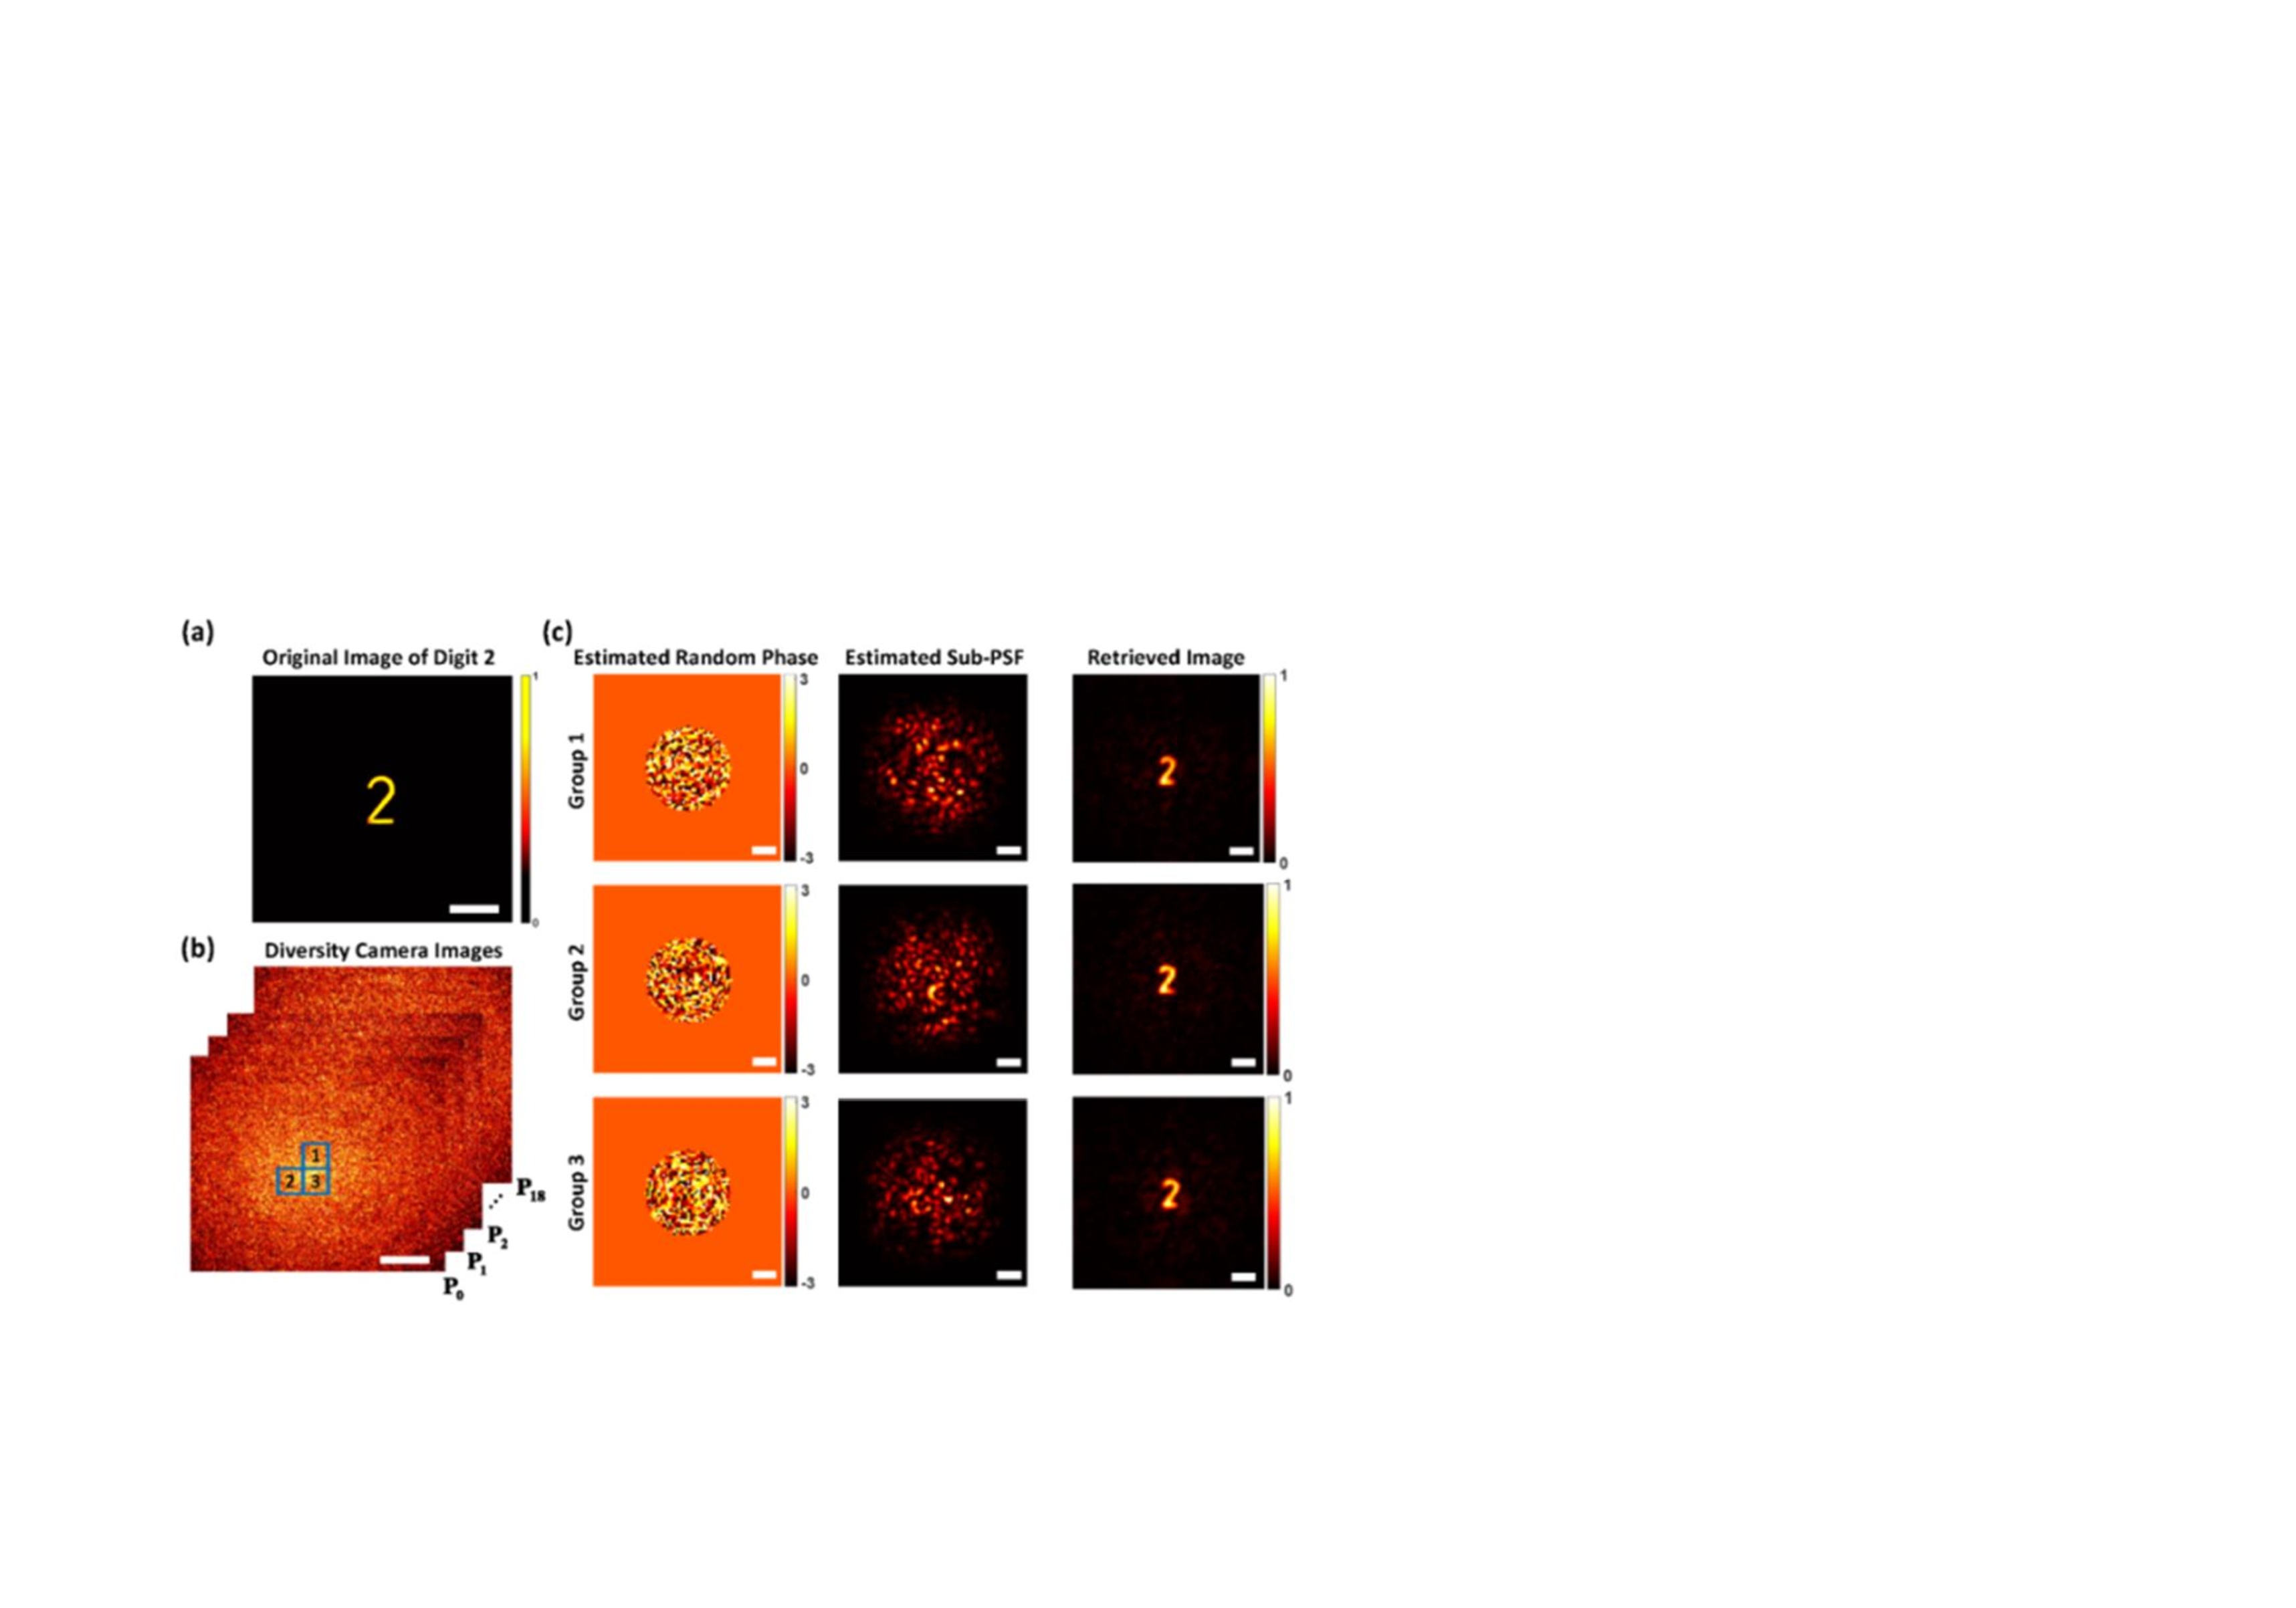
\includegraphics[scale=0.45]{C2.fig18}
	\caption{基于相位多样性的散射成像实验结果}
	\label{fig2:18}
\end{figure}

毫无疑问,基于点扩展函数工程的方法比透过散射介质成像方法具有较大优势:与波前整形相比,无需复杂的波前反馈调制及迭代,仅通过单帧散斑便可实现透过散射介质成像;与散斑相关相比,避免了相位恢复算法带来的不确定性(如位置信息和方向信息的不确定性),在光谱成像和三维成像方面有着巨大的潜力。然而,基于点扩展函数工程的方法也有不足之处:1)需要获取系统的点扩展函数,在实际应用中往往需要对点扩展进行测量,在实际应用中的难度较大;2)目标重建效果受重建算法的影响较大,选择合适的去卷积算法对重建效果具有重要;3)重建效果受限于光学系统的稳定性,任何器件的移动都可能导致重建结果失效。总而言之,基于点扩展函数工程的方法对于过散射在未来透过散射介质的三维成像和光谱成像具有重要意义。

\section{本章小节}

本章围绕当前散射成像技术的研究现状展开叙述,对波前整形和基于光学记忆效应的散射成像技术进行介绍,并对散射成像技术在生物医学领域的应用前景进行了展望。波前整形技术(光学相位共轭技术、基于反馈调节的波前整形技术和光学传输矩阵技术)的关键在于研究光在散射介质中的传播特性,利用数学的形式对散射介质的特性进行定量或定性表示。研究结果表明,利用波前整形技术可以实现透过散射介质聚焦和成像,这在生物医学利用上具有重要意义。在基于光学记忆效应的散射成像技术中,散斑相关成像通过自相关计算恢复了目标的傅里叶振幅,利用相位恢复算法恢复了傅里叶相位,从而实现了非侵入式透过散射介质成像;基于点扩展函数工程的透过散射成像技术利用点扩展函数的退相关特性和随机编码特性,实现了光谱成像和三维成像。总体来看,光学记忆效应、传输矩阵特征值的双模分布、时间反演法等物理概念,均是将电子学、声学的研究中的物理概念迁移到光学研究中,并且一一得到了验证,这为科研人员研究光散射问题指明了一个方向,即可以用某些研究电子散射问题的方法来解决光散射问题,这一事实同时也从另一角度证明了光现象和电磁现象的统一性。

综合相关文献及报道来看,散射成像技术有以下重点、难点亟需突破:1)波前整形技术的实时性仍需进一步提高,在实际应用过程中,散射介质往往具有时变特性,难以实现透过动态散射介质成像,可采用一种快速且准确的光学传输矩阵测量方法,实现透过动态散射介质聚焦或成像;2)目前的大部分波前整形技术的能量利用率较低,可设计一种能量利用率高且便于操控的波前整形技术,在更高能量利用率且快速的前提下实现透过散射聚焦;3)目前已有的波前整形技术无法实现透过散射介质的实时观测,需要设计一种无需重建过程的透过散射介质成像方法,如通过光学补偿的方式实现透过散射介质的实时成像;4)目前基于散斑相关成像方法的成像范围受限于光学记忆效应,拓展光学记忆效应的范围是未来研究的趋势,如通过研究散射介质的物理特性,利用介质自身物理特性(开通道和闭通道)实现光学记忆效应的拓展,从而实现透过散射介质大视场成像;5)所有的基于点扩展函数工程的透过散射介质成像技术都需要提前测量系统的点扩展函数,如何实现无须测量点扩展函数实现成像是未来的研究难点。

除了解决上述难点问题以外,透过散射介质成像未来较有意义的研究方向为:1)如何实现介质内的快速聚焦或成像,这将对生物医学观测或疾病检测具有重要意义;2)目前的部分研究结果表明,大气或云雾等自然界复杂介质具有散射特性,研究大气或云雾等复杂介质形成散斑的条件,实现透过自然界复杂介质成像对远距离探测和信息感知具有重要意义;3)目前大部分透过散射介质成像的方法只能实现单一物理量的探测,如何通过单帧散斑实现多物理量的探测,对目标信号的探测、识别和分辨具有重要意义;4)随着微纳加工技术的进一步发展,通过定制散射介质实现定制成像,将会对新型化、小型化和集成化的探测成像系统的发展具有深远意义;5)随着深度学习和人工智能技术的发展,可将人工智能技术引入到散射成像,通过少量先验知识或通过先验知识迁移的方式实现透过散射介质成像。

综上所述,散射成像已在光学显微、光通信和生物医学领域取得了一系列成果,但是许多问题仍待解决。散射成像技术将向着更高分辨率、更远作用距离和更快速的方向发展。可以预见,随着科研人员对光散射问题的深入研究,上述问题都能够被有效解决,并且会有更多的突破性进展,使散射成像技术能够被广泛应用于人们的日常生活及生产中。
